\chapter{DepthInSpace: Depth Estimation with Structured-Light Sensors} \label{sec:chapter2}

\begin{tcolorbox}[colback=gray!20, boxrule=1pt, colframe=black]
  Disclaimer: This chapter is adapted from the following article – with permissions of all co-authors and the conference: \\

    \textbf{Johari, M. M.}, Carta, C., and Fleuret, F. (2021). DepthInSpace: Exploitation and Fusion of Multiple Video Frames for Structured-Light Depth Estimation. In \textit{Proceedings of the IEEE/CVF International Conference on Computer Vision (ICCV)}, pages 6039-6048.
\end{tcolorbox}

\section{Chapter Abstract}

We present DepthInSpace, a self-supervised deep-learning method for depth estimation using a structured-light camera. The design of this method is motivated by the commercial use case of embedded depth sensors in nowadays smartphones. We first propose to use estimated optical flow from ambient information of multiple video frames as a complementary guide for training a single-frame depth estimation network, helping to preserve edges and reduce over-smoothing issues. Utilizing optical flow, we also propose to fuse the data of multiple video frames to get a more accurate depth map. In particular, fused depth maps are more robust in occluded areas and incur less in flying pixels artifacts. We finally demonstrate that these more precise fused depth maps can be used as self-supervision for fine-tuning a single-frame depth estimation network to improve its performance. Our models' effectiveness is evaluated and compared with state-of-the-art models on both synthetic and our newly introduced real datasets. The implementation source code, training recipe, and both synthetic and captured real datasets are available in the following link: \href{https://www.idiap.ch/paper/depthinspace}{https://www.idiap.ch/paper/depthinspace}.

\section{Chapter Introduction}

With the advent of structured-light cameras, depth-sensing became conceivable with basic algorithms implementable on devices with computational constraints in real-time. For instance, Kinect V1 uses a correlation-based block matching technique~\cite{scharstein2002taxonomy}, and Intel RealSense~\cite{keselman2017intel} employs a semi-global matching scheme~\cite{hirschmuller2007stereo}. However, learning-based approaches in this field are relatively limited. \cite{ryan2017low} propose a computationally efficient feature matching method. Projecting image patches to compact binary representation is proposed in UltraStereo~\cite{fanello2017ultrastereo} to achieve a low complex matching scheme. HyperDepth~\cite{ryan2016hyperdepth} casts the problem of depth estimation as a classification-regression task, which it solves using an ensemble of cascaded random forests. However, HyperDepth assumes the availability of ground-truth labels either from high-accuracy sensors or exhaustive stereo-matching search algorithms.

Due to the lack of large-scale, precise ground-truth data, an end-to-end training of a deep neural network in a self-supervised manner has been at the center of attention recently. ActiveStereoNet~\cite{zhang2018activestereonet} uses Siamese networks for predicting disparity and proposes a novel photometric loss function based on a Local Contrast Normalization (LCN) scheme for training. A separate color sensor is used in~\cite{kleitsiotis2019color} to enhance the performance of~\cite{zhang2018activestereonet}. \cite{riegler2019connecting} exploit the photometric loss function of ~\cite{zhang2018activestereonet} and propose an edge-detection network along with an edge-aware smoothness loss function to overcome the issue of edge fattening. They also introduce another loss function that leverages the information of other video frames to supervise the disparity estimation network's training. To do so, they use the estimated disparity and camera pose parameters to transform pixels into a 3D point cloud and apply the consistency of predicted depth of matched pixels across multiple frames. 

We take the work in~\cite{riegler2019connecting} as the baseline, and our contributions in this article are as follows:
\begin{itemize}
\item We propose a novel training scheme that uses optical flow predictions from ambient images to find matched pixels independently of the estimated disparities, which stabilizes the training and enhances accuracy. Our sensor can capture ambient images conveniently, and we exploit this feature in this regard.
\item We extend this model to fuse information from multiple video frames to obtain more precise disparity maps with sharper edges and fewer artifacts.
\item We finally propose to exploit the resulting fused disparity maps to fine-tune a single-frame disparity estimation network.
\end{itemize}

\section{Related Works} \label{sec:c2_related_work}

\noindent\textbf{Active Depth Estimation:} The setup usually consists of a camera and a projector which projects a random but known pattern of dots into the scene. Dependent on the depth of objects in the environment, the camera receives a deformed shape of the projected pattern, and this phenomenon could be used in depth estimation algorithms. Such algorithms include basic searching for correspondences in Kinect V1~\cite{martinez2013kinect}, computationally efficient learning-based techniques~\cite{fanello2017ultrastereo, ryan2016hyperdepth, chen2014fast}, and a deep neural network trained end-to-end to estimate disparity map directly~\cite{zhang2018activestereonet, kleitsiotis2019color, riegler2019connecting}.

\bigbreak\noindent\textbf{Leveraging Multiple Frames:} Utilizing multiple frames for depth estimation includes but is not limited to to structured-light sensors~\cite{riegler2019connecting}. In~\cite{godard2017unsupervised, xie2016deep3d, kuznietsov2017semi}, the second image of a stereo camera is regarded as another video frame. Explicit utilization of multiple video frames of a conventional camera for self-supervision is proposed in~\cite{zhan2018unsupervised, zhou2017unsupervised, bian2019unsupervised, godard2019digging, guizilini20203d, pillai2019superdepth, casser2019unsupervised}. Fusing the information of multiple frames during inference is employed in RGB depth estimation models like 
DeepV2D~\cite{teed2019deepv2d}, DeepMVS~\cite{huang2018deepmvs}, DeepSFM~\cite{wei2020deepsfm}, and DPSNet~\cite{im2018dpsnet} in the form of aggregating volume cost representations. In these papers, the aggregation is done by simple pooling operations (DeepV2D and DeepMVS) or performing convolution on the 2D grid (DeepSFM and DPSNet). Such approaches would fail in the context of structured-light images, where the projector also moves with the camera. As a result of the moving projector, the scene is textured with the projected dots differently, and the camera captures an entirely new scene at each frame. Simply warping frames together and aggregating on the 2D grid will limit the performance since the dots information is meaningless in the warped frames and interferes with the fusion process. We tackle this issue in Section~\ref{sec:c2_muti-frame}, where we perform fusion and convolution in the continuous 3D space to leverage the consistency of geometry there maximally. Unfortunately, all the aforementioned models are designed to work with RGB images, and we cannot evaluate them for structured-light images through experiments. However, we examine how the aggregation of frames on the 2D grid would fail for these images in the supplementary material.

\bigbreak\noindent\textbf{Optical Flow and Depth Estimation:} Numerous researches in passive depth estimation suggest taking advantage of consistency between optical flow prediction and camera ego-motion between consecutive video frames. The authors in~\cite{wang2019unos, yin2018geonet, zou2018df, ranjan2019competitive} claim that simultaneously training an optical flow network and a depth estimation network can benefit both tasks and result in a better performance than training those individually. The work in~\cite{luo2020consistent} proposes a novel framework capable of fine-tuning a general monocular depth estimation network during test time by leveraging a pre-trained optical flow estimation network. Although it is not common in the context of active stereo depth sensing, there is adequate ambient information in captured images to exploit and predict optical flow between frames and improve the quality of depth estimation accordingly.

\bigbreak\noindent\textbf{Convolution in Point Cloud:} In the context of point cloud processing, some novel techniques are proposed that perform convolution on points in the continuous 3D space resembling convolutional neural networks of regular grid structures. Models in~\cite{thomas2019kpconv, li2018pointcnn, xu2018spidercnn, wu2019pointconv, boulch2020convpoint, wang2018deep} are shown to be capable of applying convolution on unstructured and unordered data and work well on point cloud benchmark tasks and datasets. For 2D grid-style data, when depth information is available, it is plausible to transform points into the 3D space and leverage such continuous convolutions. Such an approach is presented in~\cite{chen2019learning}, where the authors jointly benefit from conventional 2D convolution and parametric continuous convolution introduced in~\cite{wang2018deep}.

\section{Method}

\begin{figure}[t]
    \begin{center}
        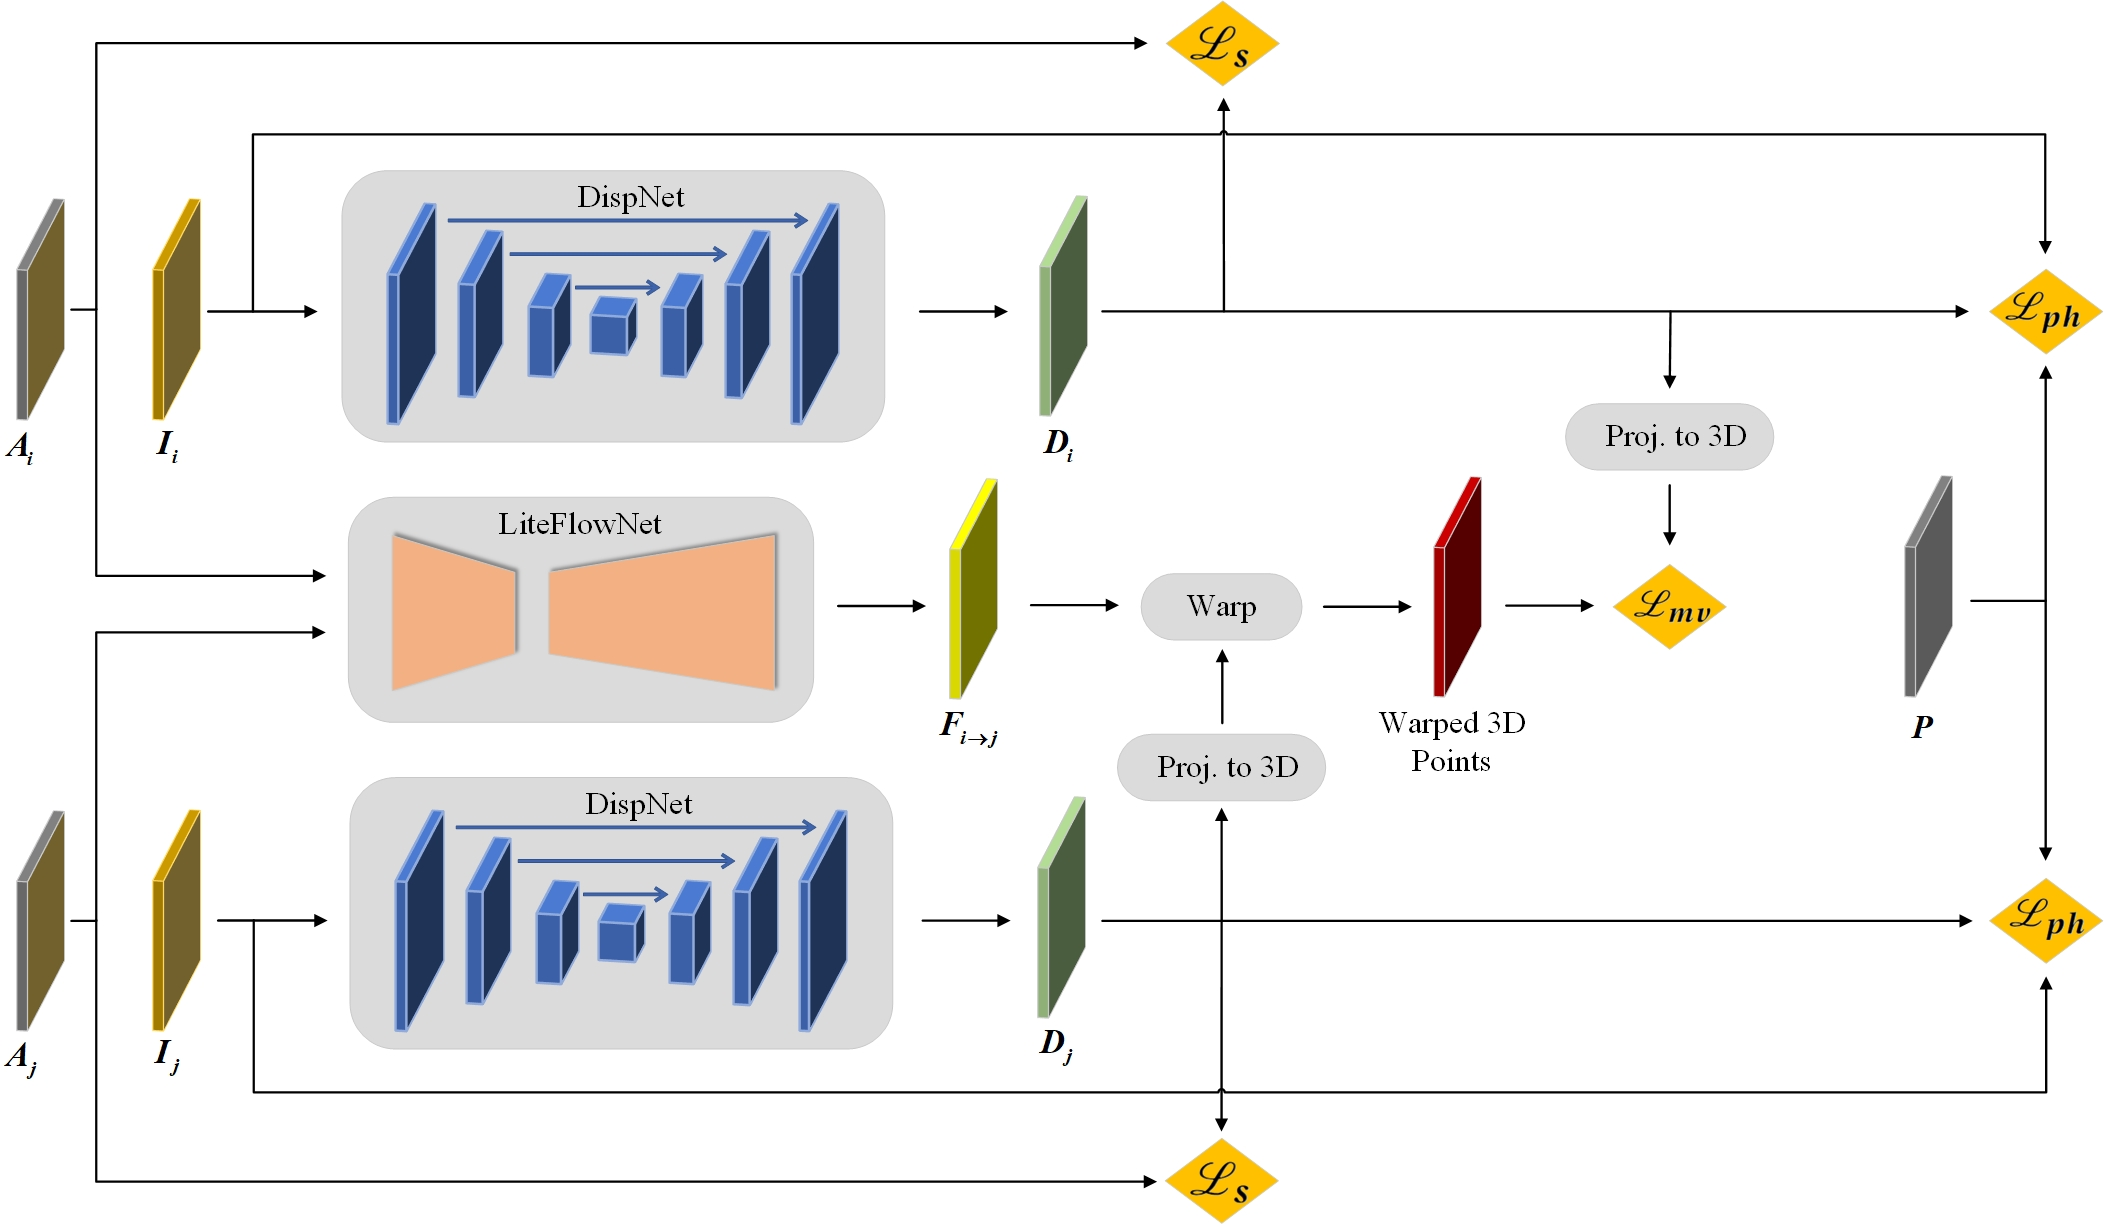
\includegraphics[width=1.0\linewidth]{images/chapter2/figures/Fig1.jpg}
    \end{center}
   \caption{The training scheme of our DIS-SF model for a sample pair of frames~$i$ and $j$, and a reference pattern~$\boldsymbol{P}$. The dot images~$\boldsymbol{I_i}$ and $\boldsymbol{I_j}$ are fed to the DispNet~\cite{mayer2016large} separately to predict disparities~$\boldsymbol{D_i}$ and $\boldsymbol{D_j}$. On another path, LiteFlowNet~\cite{hui2018liteflownet} generates optical flow of these two frames~$\boldsymbol{F_{i \rightarrow j}}$ exploiting ambient images~$\boldsymbol{A_i}$ and $\boldsymbol{A_j}$ jointly. The photometric loss~$\boldsymbol{\mathcal{L}_{ph}}$ and the smoothness loss~$\boldsymbol{\mathcal{L}_s}$ are applied to images separately, whereas the multi-view loss~$\boldsymbol{\mathcal{L}_{mv}}$, which imposes consistency of predicted depths between two frames, is applied pairwise (see Section~\ref{sec:c2_loss}). This scheme is employed for every pair of images from the same scene. The block \textbf{Warp} denotes bilinear 2D warping via optical flow and the block \textbf{Proj. to 3D} means projecting points into 3D space using the disparities and the camera's intrinsic parameters and adjusting the view angle of points using the camera's extrinsic parameters. After training and for disparity inference, DispNet~\cite{mayer2016large} takes a single dot image $\boldsymbol{I}$ and estimates a disparity map $\boldsymbol{D}$ as output.}
    \label{fig:c2_single}
\end{figure}

We build DepthInSpace (DIS) model upon the Connecting the Dots (CTD) model in~\cite{riegler2019connecting}. CTD suggests using two separate networks, one for estimating the disparity, and the other for detecting the edges in the images. The edge detector is weakly supervised with the ambient images, which are the same as dot images except that the projector is off during photo capture. Obtaining ambient data is considerably cheaper than the ground-truth depth data; however, the edge detection network is proposed to reduce the number of ambient images required for training.

We claim ambient images contain more valuable information than only the objects' edges. The sensor that we use is equipped with a programmable switch that can capture both dot images and ambient images with no additional cost. Accordingly, we discard the edge detection network and replace the CTD's smoothing loss function with a loss that directly extracts edges from ambient images. Also, we predict the optical flow from ambient images to find the matched pixels and introduce a new loss which encourages geometric consistency between them. Our proposed loss replaces the geometric loss in CTD and is preferable in two regards. First, CTD uses the momentary predicted depth and ego-motion of the camera to find the matched pixels. As a result, the optimization landscape changes rapidly during training and could result in instability of training. Secondly, the error in momentary predicted depths participates in the procedure of finding matched pixels and leads to degraded performance. In addition, the matching scheme with optical flow provides more flexibility to detect mistakenly matched pixels and exclude them from contributing to the loss function. We use LiteFlowNet~\cite{hui2018liteflownet} pre-trained on MPI Sintel~\cite{butler2012naturalistic} for optical flow, which is a lightweight and fast model, but it has comparable performance to computational and memory resource expensive models like FlowNet2~\cite{ilg2017flownet}.

\subsection{Single-Frame Disparity Estimation} \label{sec:c2_single-frame}

Our DepthInSpace Single-Frame (DIS-SF) model takes the CTD model~\cite{riegler2019connecting} as a baseline and modifies two of its loss functions: we incorporate a novel multi-view loss function leveraging optical flow predictions and an improved edge-aware smoothness loss. The training scheme of our DIS-SF model is presented in Figure~\ref{fig:c2_single}. The photometric loss~$\boldsymbol{\mathcal{L}_{ph}}$ enforces consistency between the input image and the warped reference pattern via the estimated disparity map. For smoothness loss~$\boldsymbol{\mathcal{L}_{s}}$, we propose using an edge-aware one similar to~\cite{godard2017unsupervised, godard2019digging, pillai2019superdepth}, except that we extract the edge information directly from the ambient images.

Furthermore, we introduce a novel multi-view loss~$\boldsymbol{\mathcal{L}_{mv}}$, which enforces the consistency of the estimated depths between two different views with the help of bilinear warping via optical flow predictions. Note that the photometric loss and smoothness loss apply to each image individually, whereas the multi-view loss applies to all possible permutations of image pairs from the same scene. For more details about the loss functions, refer to Section~\ref{sec:c2_loss}.

We use DispNet~\cite{mayer2016large} for inferring disparity. We also apply Local Contrast Normalization (LCN) preprocessing, suggested in~\cite{zhang2018activestereonet, riegler2019connecting}, to both dot images~$\boldsymbol{I}$ and the reference pattern~$\boldsymbol{P}$. Although we use ambient images $\boldsymbol{A}$ in our training scheme, we do not directly employ them as DispNet's input. This makes data preparation more convenient during inference, and DispNet~\cite{mayer2016large} predicts disparity maps $\boldsymbol{D}$ only based on dot images $\boldsymbol{I}$. Instead, the pairs of ambient images are exploited as the input of LiteFlowNet~\cite{hui2018liteflownet} to predict the optical flow map~$\boldsymbol{F}$. More discussion on how we use pre-trained LiteFlowNet with ambient images, while it is designed to work with RGB images, as well as an ablation study are provided in the supplementary.

\subsection{Multi-Frame Disparity Estimation} \label{sec:c2_muti-frame}

Our Multi-Frame (DIS-MF) model combines the information of other frames from the same scene into one frame and generates more accurate disparities. We assume an initial imperfect disparity map is available for each frame beforehand, and we attempt to increase the quality of the disparities by fusing the frames. In this regard, we take the outputs of our DIS-SF model as the imperfect disparities. Compared to traditional RGB depth estimation, aggregating data of multiple frames is more efficacious in structured-light setup because the performance of depth sensing depends on how the dots touch the objects in the environment. Thus, the data contained in the frames are less correlated.

Let~$\boldsymbol{\phi} \in \mathbb{R}^{C \times H \times W}$ denote a feature map of size~$H \times W$ with~$C$ channels, and~$\boldsymbol{X} \in \mathbb{R}^{3 \times H \times W}$ denote the corresponding 3D points obtained using the imperfect disparities and camera projection matrix~$\boldsymbol{K} \in \mathbb{R}^{3 \times 3}$. Let us assume we have a pair of images with feature maps of~$(\boldsymbol{\phi_i},\boldsymbol{\phi_j})$ and 3D points of~$(\boldsymbol{X_i},\boldsymbol{X_j})$. Frame $i$ is assumed as the target frame, and we want to fuse the information of~$\boldsymbol{\phi_j}$ into~$\boldsymbol{\phi_i}$. Our model's first step is warping both feature map~$\boldsymbol{\phi}$ and 3D points~$\boldsymbol{X}$ on the 2D grid via optical flow predictions~$\boldsymbol{F_{i \rightarrow j}}$ and $\boldsymbol{F_{j \rightarrow i}}$. Optical flow warping places the data of the frames on the 2D grid such that corresponding data of the frames appear in each other's neighborhood on the 2D grid.

Let $\boldsymbol{\phi_{j \rightarrow i}}=w^{j \rightarrow i}(\boldsymbol{\phi_j})$ and $\boldsymbol{X_{j \rightarrow i}}=w^{j \rightarrow i}(\boldsymbol{X_j})$ denote warped features and warped points, where $w^{j \rightarrow i}(\cdot)$ stands for bilinear 2D warping via the optical flow $\boldsymbol{F_{i \rightarrow j}}$. We also define a binary mask map~$\boldsymbol{M_{j \rightarrow i}} \in \{0,1\}^{1 \times H \times W}$ which indicates if the warped data is valid and should be allowed to participate in our fusion framework. We construct $\boldsymbol{M_{j \rightarrow i}}$ by evaluating the forward-backward consistency of optical flow predictions, similar to \cite{zou2018df,meister2017unflow}:
\begin{multline}\label{eqn:flow_forward_backward}
    \boldsymbol{M_{j \rightarrow i}} = |\boldsymbol{F_{i \rightarrow j}} + w^{j \rightarrow i}(\boldsymbol{F_{j \rightarrow i}})|^2\\
    < 0.01 \times (|\boldsymbol{F_{i \rightarrow j}}|^2 + |w^{j \rightarrow i}(\boldsymbol{F_{j \rightarrow i}})|^2) + 0.5
\end{multline}

Despite having all warped data and their validation mask map on the same 2D grid, we do not perform fusion naively on the grid space. As we already mentioned in Section~\ref{sec:c2_related_work}, warped features in the structured-light setup contain interfering data of warped dots that make the fusion task complicated. Instead, we propose a fusion block that performs fusion and convolution in the continuous 3D space. Our fusion block also has a sense of faulty imperfect disparities and can prevent those points from contributing to the aggregation. The details of our fusion block and its utilization in our DIS-MF network architecture are as follows.

\begin{figure}[t]
    \begin{center}
        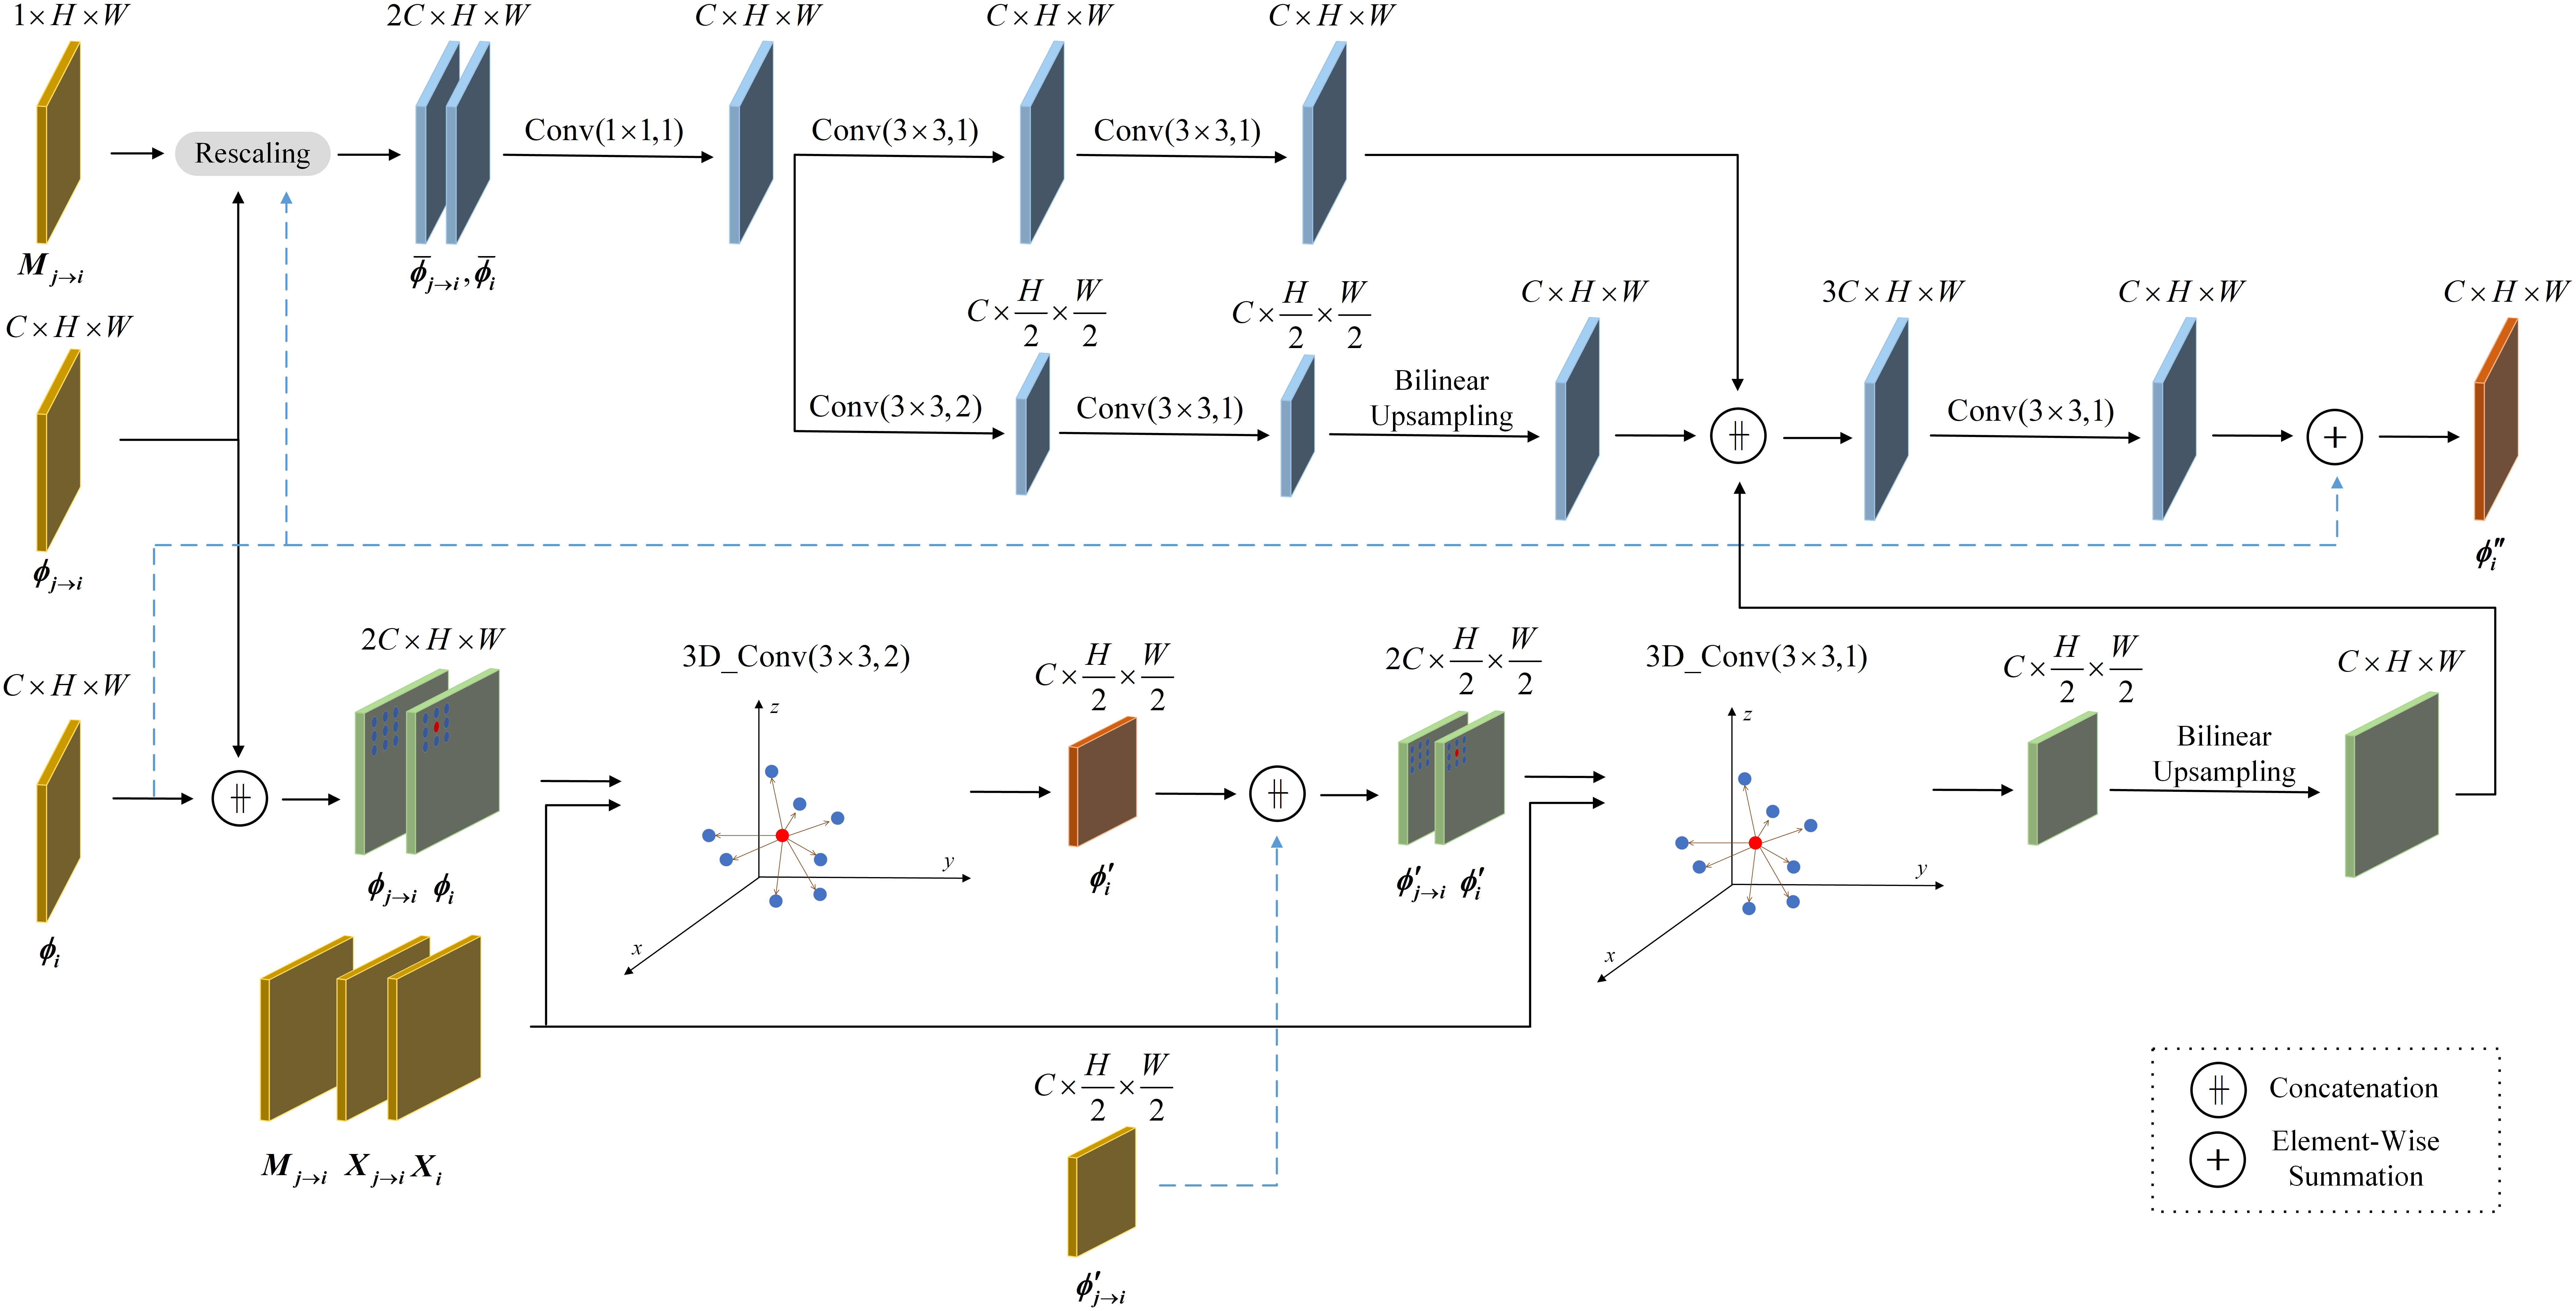
\includegraphics[width=1.0\linewidth]{images/chapter2/figures/Fig2.jpg}
    \end{center}
   \caption{Internal architecture of our proposed fusion block, whose details of utilization in our DIS-MF model are illustrated in Section~\ref{sec:c2_muti-frame} and Figure~\ref{fig:c2_architecture}. We depict how features of an auxiliary frame~$\boldsymbol{\phi_{j \rightarrow i}}$ are being fused into the target frame's features~$\boldsymbol{\phi_{i}}$. Binary mask map~$\boldsymbol{M_{j \rightarrow i}}$, 3D points of the target frame~$\boldsymbol{X_{i}}$ and warped frame~$\boldsymbol{X_{j \rightarrow i}}$, and the warped result of the first 3D convolution of the auxiliary frame~$\boldsymbol{\phi'_{j \rightarrow i}}$ are also inputs of this block. $\boldsymbol{\phi''_{i}}$ stands for the output of this block, and $\boldsymbol{\phi'_{i}}$ represents the output of the first 3D convolution required for fusing into other frames' fusion blocks. $\text{Conv}(k \times k, s)$ and $\text{3D\textunderscore Conv}(k \times k, s)$ denote 2D and continuous 3D convolution respectively, with kernel size of $k$ and stride $s$, and the block \textbf{Rescaling} denotes the operations described in Equation~\eqref{eqn:rescaling}.}
    \label{fig:c2_fusion}
\end{figure}

\bigbreak\noindent\textbf{Fusion Block:} \cite{chen2019learning} suggest when depth information of a 2D image is available, it is conceivable to exploit continuous convolution in the 3D space and benefit from both 2D and 3D data processing simultaneously. Such a proposal is consistent with the idea of merging the data of multiple frames as the projected points in the 3D space could be processed regardless of their camera pose. Inspired by them, we propose a fusion block capable of fusing several feature maps originating from different frames into the target frame's feature map. For the sake of simplicity, let us assume we only have two frames and intend to merge the feature map~$\boldsymbol{\phi_j}$ into the target feature map~$\boldsymbol{\phi_i}$. The functionality of the fusion block is illustrated in Figure \ref{fig:c2_fusion}. We use the continuous 3D convolution~\cite{wang2018deep} as the core element of our fusion block. Most architectures that exploit 3D convolution on the point cloud require running exhaustive search algorithms to find points in the neighborhood~\cite{chen2019learning, li2018pointcnn, xu2018spidercnn, wu2019pointconv, boulch2020convpoint, wang2018deep}, which is infeasible to perform on dense data such as ours. For instance,  \cite{chen2019learning} pre-compute the indices of nearest neighbors for all points. To mitigate the issue, we propose a novel technique that is practical in real-time processing. Since our data is not fully unstructured, we suspect points that are close in 3D space will be close on the 2D grid map if they are warped to the same camera perspective, but not vice versa. 

Accordingly, we form the concatenated feature map~$[\boldsymbol{\phi_{j \rightarrow i}},\boldsymbol{\phi_{i}}]$ and point map~$[\boldsymbol{X_{j \rightarrow i}},\boldsymbol{X_{i}}]$ and slide a $3\times3$ window over each 2D grid map simultaneously and perform convolution only on points inside the sliding window similarly to a conventional CNN. The difference is, instead of performing a weighted sum with learnable parameters, we search for the nearest points and perform continuous convolution. For simplifying the equations, let $\boldsymbol{\phi_{i \rightarrow i}}=\boldsymbol{\phi_{i}}$, $\boldsymbol{X_{i \rightarrow i}}=\boldsymbol{X_{i}}$, and $\boldsymbol{M_{i \rightarrow i}}=\vec{\mathbf{1}}$. Also, let $\boldsymbol{\phi}(h,w)$ and $\boldsymbol{X}(h,w)$ represent the features and the coordinate of the position $(h,w)$ on the grid map where $0 \le h < H$ and $0 \le w < W$. We first search for the nearest points to the center point of the sliding window on the target frame $i$:
\begin{multline} \label{eqn:search_neighbors}
l^*(h,w),m^*(h,w),n^*(h,w) 
\\= \underset{\substack{l \in \{i,j\} \\ -1\le m \le +1 \\ -1 \le n \le +1}}{\textit{k-}\!\arg\min} \ 
\frac{\big| \boldsymbol{X_{l \rightarrow i}}(h+m,w+n) - \boldsymbol{X_{i}}(h,w)\big|}{\boldsymbol{M_{l \rightarrow i}} + \epsilon}
\end{multline}
where $\textit{k-}\!\arg\min g(\cdot)$ returns the $k$ indices that minimize the function $g(\cdot)$, and $\epsilon$ is a small constant. $\boldsymbol{M_{l \rightarrow i}}$ is used in the denominator to exclude invalid points, and we set $k=9$ to ensure all returned indices correspond to valid pixels due to the window size $3 \times 3$. To extend the model to fuse more than two frames, $l$ in Equation~\ref{eqn:search_neighbors} should span all available frames rather than only $\{i,j\}$. The convolution's result is:
\begin{multline}
\! \! \! \! \boldsymbol{\phi'_{i}}(h,w)= \Psi \times \! \! \! \! \sum_{l^*,m^*,n^*} \! \! \!
\Big( \! \boldsymbol{\phi_{l^* \rightarrow i}}(h+m^*,w+n^*) \ \\ \odot \ \text{MLP}\big(\boldsymbol{X_{l^* \rightarrow i}}(h+m^*,w+n^*) - \boldsymbol{X_{i}}(h,w)\big) \Big)
\end{multline}
where MLP is a multi-layer perceptron mapping 3D vectors to $C$-dimensional weights, $\odot$ denotes element-wise product, and $\Psi$ is a $C \times C$ learnable weight matrix. This implementation can be regarded as a continuous version of separable convolution. The MLP and weighted sum perform depth-wise convolution, while the linear transformation resembles $1 \times 1$ convolution~\cite{chen2019learning}.

As shown in Figure~\ref{fig:c2_fusion}, we adopt two 3D convolutions in each fusion block. Accordingly, we warp the other frames' outputs of the first 3D convolution to the target frame~$\boldsymbol{\phi'_{j \rightarrow i}}$ and fuse them into the second 3D convolution as well. We also employ traditional 2D CNNs in the fusion block because there are some shortcomings to 3D convolution, such as edge fattening near the boundaries of objects and background. To merge the feature maps in 2D CNNs, we handle invalid points differently by proposing a scheme similar to dropout~\cite{srivastava2014dropout}. To do so, we first zero out features of invalid points, and then rescale the remaining valid features inversely proportionally to the number of valid frames for each point on the 2D grid:
\begin{equation}\label{eqn:rescaling}
\forall l \in \{i,j\}: \boldsymbol{\bar{\phi}_{l \rightarrow i}} = \frac{\boldsymbol{\phi_{l \rightarrow i}} \times \boldsymbol{M_{l \rightarrow i}}}{\displaystyle{\sum_{p \in \{i,j\}} \! \! \! \boldsymbol{M_{p \rightarrow i}}}}
\end{equation}

The 3D convolutions along with 2D CNNs jointly construct the fusion block, which is capable of processing high-resolution feature maps and effectively benefits from the information of other frames from the same scene. SELU nonlinearity~\cite{klambauer2017self} and Group Norm~\cite{wu2018group} are used after each convolution. We prefer Group Norm to Batch Norm~\cite{ioffe2015batch} in our model because Group Norm statistics are independent of the number of samples in a batch and make training large networks feasible with smaller batch sizes.

\begin{figure}[t]
    \begin{center}
        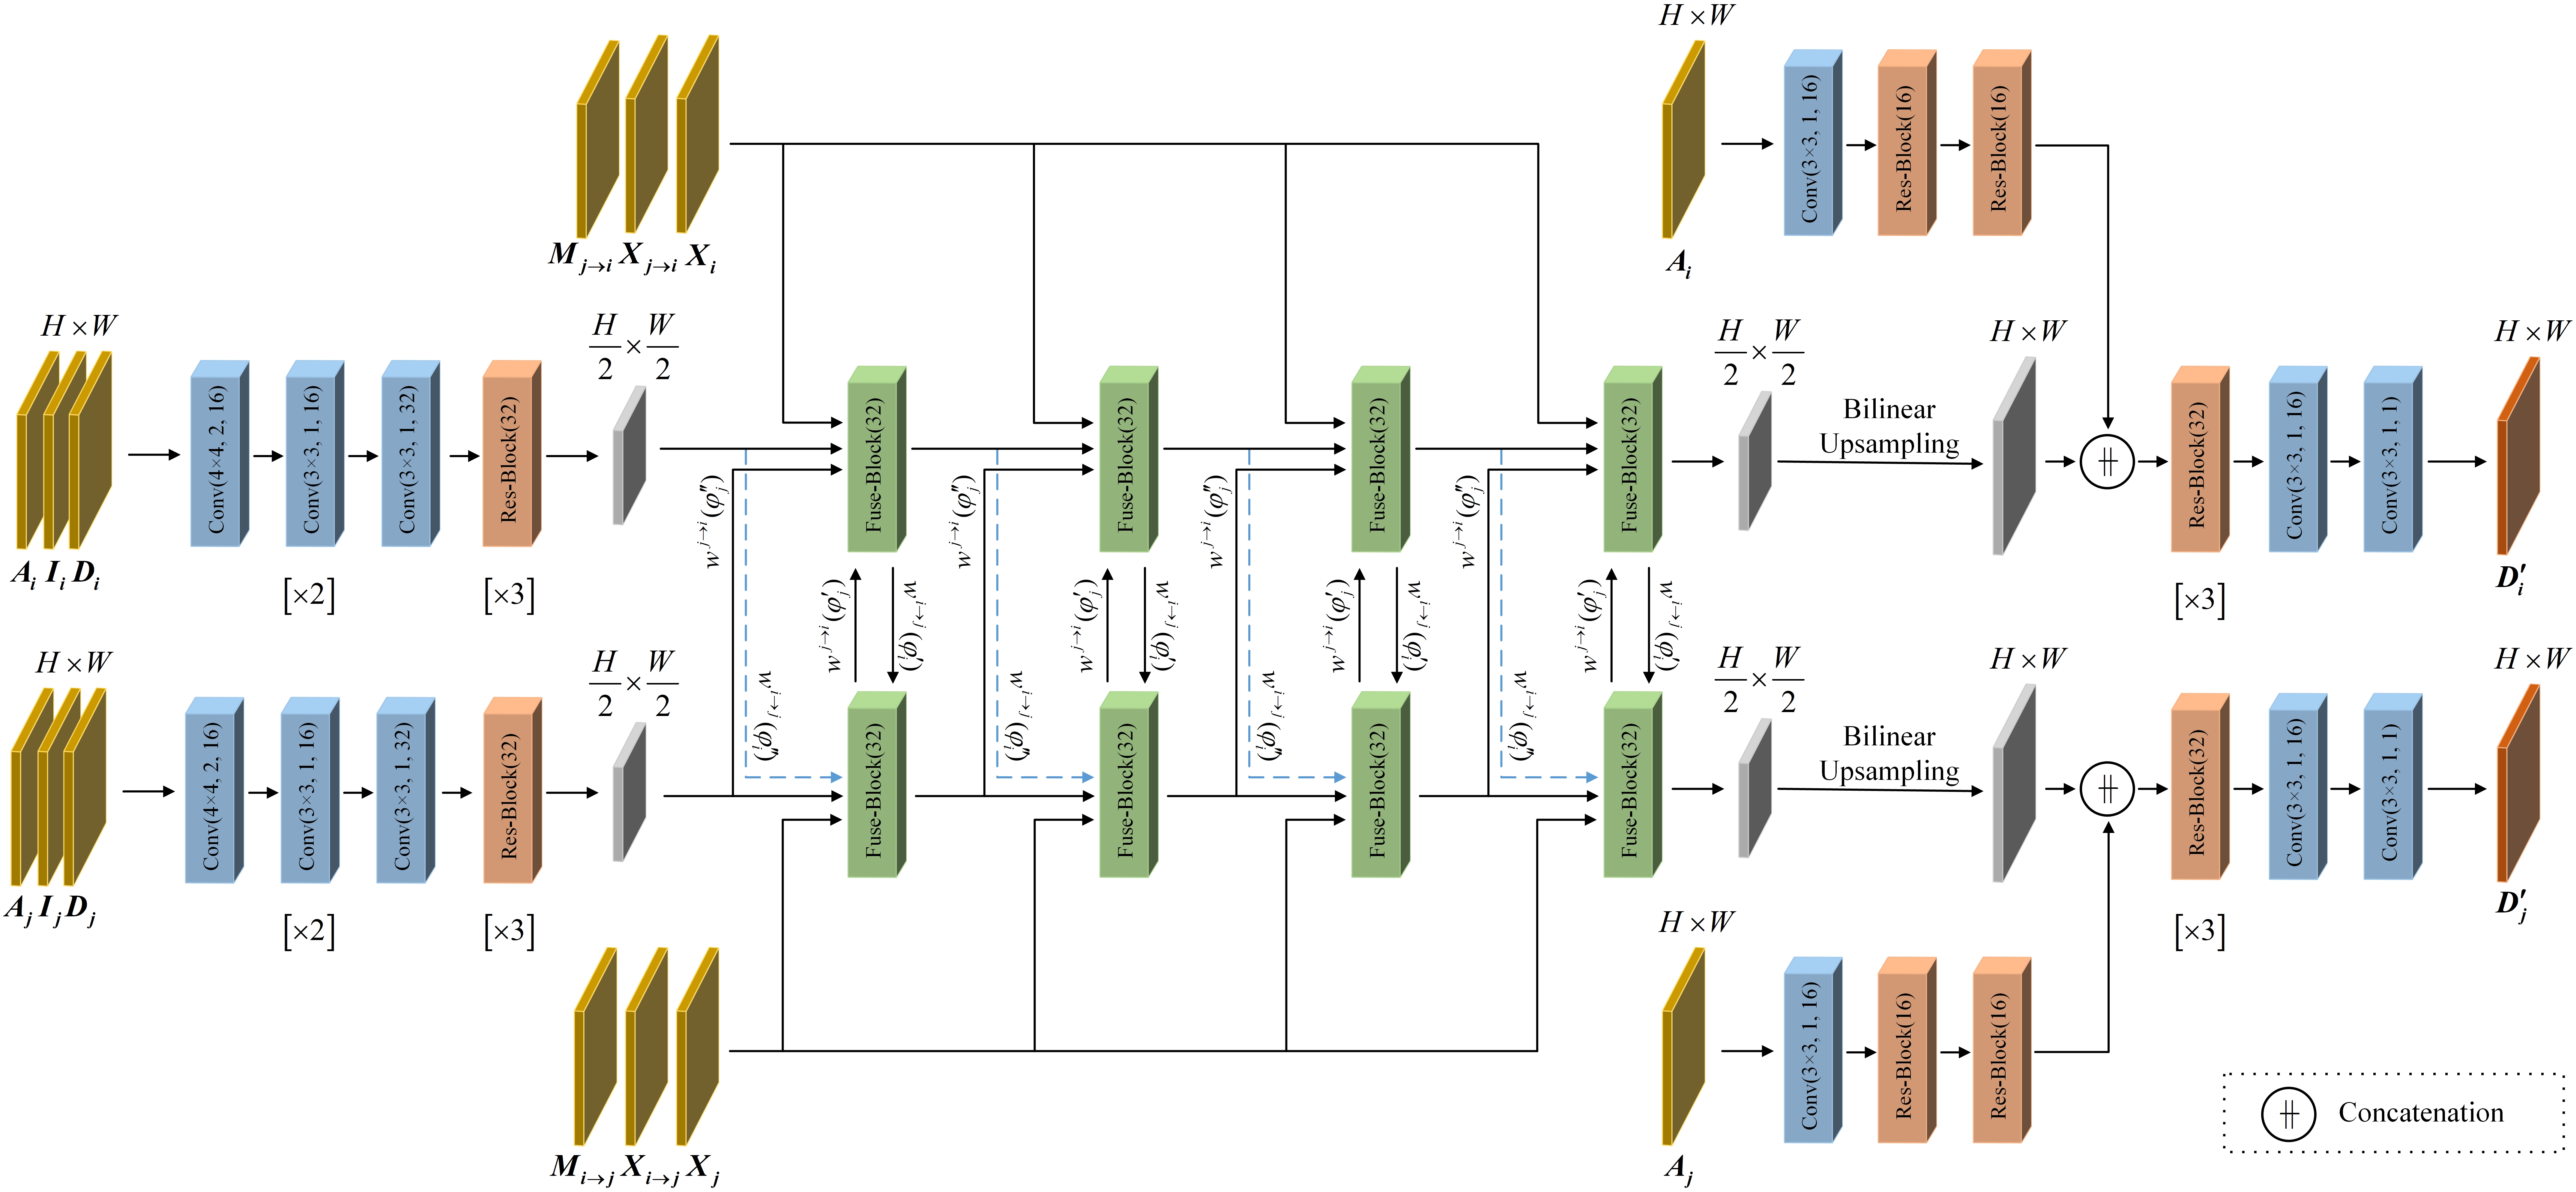
\includegraphics[width=1.0\linewidth]{images/chapter2/figures/Fig3.jpg}
    \end{center}
   \caption{Our DIS-MF network architecture when only two frames $i$ and $j$ are combined. Warping the first 3D convolution output~$\boldsymbol{\phi'}$ and the final output of each fusion block~$\boldsymbol{\phi''}$ using the relative optical flows are denoted by $w^{i \rightarrow j}(\cdot)$ and $w^{j \rightarrow i}(\cdot)$. Note that $\boldsymbol{D}$ stands for imperfect disparity participating as one of the inputs, and $\boldsymbol{D'}$ represents the final predicted disparity of the model. This figure depicts the inference network of our DIS-MF model. For training the DIS-MF model, this network replaces those individual DispNet~\cite{mayer2016large} networks in the DIS-SF model in Figure~\ref{fig:c2_single}, and the same scheme and loss functions (see Section~\ref{sec:c2_loss}) are adopted.}
    \label{fig:c2_architecture}
\end{figure}

\bigbreak\noindent\textbf{Network Architecture:} Figure~\ref{fig:c2_architecture} illustrates the network architecture of our DIS-MF model. The architecture includes three sections as follows. The preprocessing section takes the images~$(\boldsymbol{I},\boldsymbol{A})$ and the imperfect disparity~$\boldsymbol{D}$ as input and generates high-level feature maps for each frame individually. Next, the feature maps are fed into cascaded series of fusion blocks, along with their corresponding 3D points $\boldsymbol{X}$ and binary masks $\boldsymbol{M}$ required for merging and 3D convolutions to obtain fused feature maps. Warping with the optical flow is employed whenever any data on a 2D grid map is needed to be warped to another frame's 2D grid.

Lastly, the fused feature maps go through a refinement structure to preserve high-resolution details such as edges and reduce distortions resulting from combining frames. Our refinement section is inspired by the one in~\cite{zhang2018activestereonet}, but takes the upsampled fused features and the ambient image as inputs. In both the preprocessing and refinement sections, we exploited residual blocks introduced in~\cite{he2016deep} to promote gradient backpropagation and expedite the training process.

An ablation study of design choices for the DIS-MF network architecture is provided in the supplementary.

\subsection{Fine-Tuning the Single-Frame Model} \label{sec:c2_fine-tuned}

For purposes where resources are limited during inference, we propose an alternative approach to exploit the scheme of fusing image frames. We suggest that after training the DIS-MF model, the produced disparities can be used as an auxiliary loss function to supervise and fine-tune the single-frame network. The resulting model, DepthInSpace Fine-Tuned Single-Frame (DIS-FTSF), can yield more accurate disparity maps with no additional memory or computation cost during inference compared with DIS-SF.

\section{Loss Functions}\label{sec:c2_loss}

Here we introduce our loss functions employed in our models. Let $\Gamma=\{\boldsymbol{I_{i}}, \boldsymbol{A_{i}}\}_{i=0}^{N-1}$ denote the image samples from the same scene. The overall loss function consists of a photometric loss~$\boldsymbol{\mathcal{L}_{ph}}$, a smoothness loss~$\boldsymbol{\mathcal{L}_s}$, a multi-view loss~$\boldsymbol{\mathcal{L}_{mv}}$, and a pseudo-ground truth loss~$\boldsymbol{\mathcal{L}_{pgt}}$:
\begin{multline}
    \boldsymbol{\mathcal{L}} = \frac{1}{N}\sum_{i \in \Gamma} (\boldsymbol{\mathcal{L}^{i}_{ph}} + \lambda_{1}\boldsymbol{\mathcal{L}^{i}_{s}} + \lambda_{2}\boldsymbol{\mathcal{L}^{i}_{pgt}})\\
    + \frac{1}{N(N-1)}\sum_{i,j \in \Gamma} \lambda_{3}\boldsymbol{\mathcal{L}^{ij}_{mv}}
\end{multline}
where $\{\lambda_{k}\}_{k=1}^{3}$ are weighting constants, which do not necessarily take the same value in all of our models.

Let~$\boldsymbol{D}$ denote the disparity map, $\boldsymbol{\tilde{I}}$ denote the local contrast normalized input image, and $\boldsymbol{P}$ denote the local contrast normalized reference dot pattern. Similarly to CTD, we employ the smooth Census transform~\cite{hafner2013census}, represented by $\parallel \cdot \parallel_{C}$, in our photometric loss:
\begin{equation}\label{eqn:photometric}
    \boldsymbol{\mathcal{L}^{i}_{ph}}=\sum_{h,w} \parallel \boldsymbol{\tilde{I}_i}(h,w) - \boldsymbol{P}\big(h,w - \boldsymbol{D_{i}}(h,w)\big) \parallel_{C}
\end{equation}

Since we assume the availability of ambient images, we introduce an edge-aware smoothness loss similar to~\cite{godard2017unsupervised,godard2019digging}. The smoothness loss imposes consistency between disparity map discontinuities and edges in the ambient image:
\begin{equation}
    \boldsymbol{\mathcal{L}^{i}_{s}}= |\nabla_{h} \boldsymbol{D_{i}}|e^{-\beta|\nabla_{h} \boldsymbol{A_{i}}|}
    +
    |\nabla_{w} \boldsymbol{D_{i}}|e^{-\beta|\nabla_{w} \boldsymbol{A_{i}}|}
\end{equation}
where $\nabla_{h}$ and $\nabla_{w}$ stand for 2D spatial gradients and $\beta$ is a constant. Moreover, we impose the consistency between the predicted depths in each pair of images from the same scene. Let $\boldsymbol{X_{i}}$ and $\boldsymbol{X_{j}}$ denote the 3D point clouds of the two frames obtained using the momentary predicted disparities and camera intrinsic matrix. Our multi-view loss is:
\begin{equation}
    \boldsymbol{\mathcal{L}^{ij}_{mv}}=
    \bigg|
    \Big \langle \boldsymbol{X_{i}} -
    w^{j \rightarrow i}
    \big( \boldsymbol{T_{j \rightarrow i}} \times [\boldsymbol{X_{j}},\vec{\mathbf{1}}] \big) \Big \rangle_z
    \bigg| \times \boldsymbol{M'_{j \rightarrow i}}
\end{equation}
where $\boldsymbol{T_{j \rightarrow i}} \in \mathbb{R}^{3 \times 4}$ is the transformation matrix consisting of ego motion parameters, $\vec{\mathbf{1}}$ is an all one matrix, and $\langle\cdot\rangle_z$ operator returns the depth $z$ of its input 3D vector. $\boldsymbol{M'_{j \rightarrow i}}$ is a binary mask map validating warped points similarly to $\boldsymbol{M_{j \rightarrow i}}$ in Section~\ref{sec:c2_muti-frame}, but it strictly excludes low confidence points from supervising the training. For more details regarding $\boldsymbol{M'_{j \rightarrow i}}$, refer to the supplementary.

Lastly, only in our DIS-FTSF model, we use the more accurate fused disparity~$\boldsymbol{D'}$ as pseudo-ground truth to improve the quality of the imperfect disparity~$\boldsymbol{D}$. We impose the L1 consistency between~$\boldsymbol{D}$ and~$\boldsymbol{D'}$ as an auxiliary loss:
\begin{equation}
    \boldsymbol{\mathcal{L}^{i}_{pgt}}=
    |\boldsymbol{D_{i}} - \boldsymbol{D'_{i}}|
\end{equation}

\section{Experiments}
\label{sec:c2_experiments}

\noindent\textbf{Datasets:} To evaluate our models and compare them with existing methods, we examine the accuracy of depth estimation on three synthetic datasets and one real dataset. We used the tool provided by CTD~\cite{riegler2019connecting} to render the synthetic data. Rendering is done in the same experimental setup as CTD with the same objects of the ShapeNet Core dataset~\cite{chang2015shapenet}, but the images are captured by a sensor whose parameters are set similar to our own hardware. One dataset is rendered using the Kinect dot pattern for projection, and the second dataset is generated utilizing our own theoretical dot pattern for the projector. For the last synthetic dataset, we projected and captured the dot pattern in a real laboratory environment and used the observed pattern for rendering the dataset. In this regard, we use a virtual projector with the same parameters of the capturing camera.

We incorporated multiple datasets because different dot patterns could lead to different depth sensing performances. The denser the dots are, the better the performance is. However, choosing a dot pattern could be restricted by hardware limitations or available illumination power. That is why we examine the models' performances over different projected dot patterns. For each synthetic dataset, we create 8192 sequences for training, 512 sequences for validation, and 512 sequences for testing. Each sequence contains 4 pair of dot images and ambient images from the same scene.

We also evaluate the models on a smaller real dataset to show the generalization of our method in an actual setup. The data include 148 sequences of 4 pairs of dot images and ambient images captured from 4 different scenes. The sensor we use is equipped with a programmable switch, enabling the projector to be on and off, so it can capture dot images and ambient images alternately at the rate of 15 fps each. Given the capturing rate, each pair of dot image and ambient image captures the same scene approximately. We put aside 18 sequences for validating and testing and utilized 130 sequences in training. To obtain accurate ground truth we used a 3D scanner, the data of which is only used for evaluation. Due to the scanner limitations, we take a set of partial scans that best cover the scene. These are fused together to create a 3D model using the point-to-plane variant of the ICP algorithm~\cite{Chen1992ObjectMB}. A 3D mesh is then produced using the Ball-Pivoting algorithm~\cite{bernardini99ball}. For estimating the camera motion parameters, the same ICP variant is used to align the ground truth 3D model and the 3D model obtained from the structured-light sensor via the block matching technique.

More details of the datasets and also implementing our models are provided in the supplementary.

\begin{table}[t]
    \begin{center}
        \begin{threeparttable}
        \begin{tabular}{l|lcccc}
        \hline
        Dataset & Method & $o(0.5)$ & $o(1)$ & $o(2)$ & $o(5)$ \\
        \hline
        \multirow{6}{*}{ \parbox{20ex}{Synthetic \\ (Kinect Pattern)}} & SGM & 10.36 & \phantom{0}9.13 & \phantom{0}8.76 & \phantom{0}2.45 \\
        & HyperDepth$^a$ & \phantom{0}4.38 & \phantom{0}3.22 & \phantom{0}2.69 & \phantom{0}2.39 \\
        & CTD & \phantom{0}2.74 & \phantom{0}1.45 & \phantom{0}0.77 & \phantom{0}0.24 \\
        & DIS-SF & \phantom{0}2.11 & \phantom{0}1.13 & \phantom{0}0.59 & \phantom{0}0.16 \\
        & DIS-FTSF & \phantom{0}\textbf{1.92} & \phantom{0}\textbf{1.00} & \phantom{0}\textbf{0.51} & \phantom{0}\textbf{0.14} \\
        \arrayrulecolor{lightgray}\cline{2-6}\arrayrulecolor{black}
        & DIS-MF & \phantom{0}1.59 & \phantom{0}0.72 & \phantom{0}0.33 & \phantom{0}0.10 \\
        \hline
        \hline
        \multirow{6}{*}{ \parbox{20ex}{Synthetic \\ (Our Pattern)} } & SGM & 12.93 & 11.64 & 11.22 & \phantom{0}4.06 \\
        & HyperDepth$^a$ & \phantom{0}7.35 & \phantom{0}6.48 & \phantom{0}6.11 & \phantom{0}5.86 \\
        & CTD & \phantom{0}3.38 & \phantom{0}1.71 & \phantom{0}0.85 & \phantom{0}0.28 \\
        & DIS-SF & \phantom{0}2.31 & \phantom{0}1.24 & \phantom{0}0.62 & \phantom{0}0.19 \\
        & DIS-FTSF & \phantom{0}\textbf{1.96} & \phantom{0}\textbf{0.95} & \phantom{0}\textbf{0.45} & \phantom{0}\textbf{0.12} \\ \arrayrulecolor{lightgray}\cline{2-6}\arrayrulecolor{black}
        & DIS-MF & \phantom{0}1.58 & \phantom{0}0.71 & \phantom{0}0.32 & \phantom{0}0.10 \\
        \hline
        \hline
        \multirow{6}{*}{ \parbox{20ex}{Synthetic \\ (Observed Pattern)} } & SGM & 12.45 & 10.37 & \phantom{0}9.55 & \phantom{0}4.83 \\
        & HyperDepth$^a$ & \phantom{0}6.13 & \phantom{0}4.92 & \phantom{0}4.34 & \phantom{0}4.00 \\
        & CTD & \phantom{0}3.76 & \phantom{0}2.25 & \phantom{0}1.03 & \phantom{0}0.37 \\
        & DIS-SF & \phantom{0}3.66 & \phantom{0}2.16 & \phantom{0}1.00 & \phantom{0}0.23 \\
        & DIS-FTSF & \phantom{0}\textbf{2.87} & \phantom{0}\textbf{1.48} & \phantom{0}\textbf{0.66} & \phantom{0}\textbf{0.17} \\ \arrayrulecolor{lightgray}\cline{2-6}\arrayrulecolor{black}
        & DIS-MF & \phantom{0}2.46 & \phantom{0}1.24 & \phantom{0}0.54 & \phantom{0}0.14 \\
        \hline
        \hline
        \multirow{6}{*}{\parbox{20ex}{Real}} & SGM$^b$ & 25.54 & 19.23 & 17.75 & 16.96 \\
        & HyperDepth$^a$ & 34.62 & 25.09 & 22.49 & 21.77 \\
        & CTD & 22.74 & \phantom{0}9.26 & \phantom{0}3.79 & \phantom{0}\textbf{1.00} \\
        & DIS-SF & 17.95 & \phantom{0}7.93 & \phantom{0}3.59 & \phantom{0}1.14 \\
        & DIS-FTSF & \textbf{17.06} & \phantom{0}\textbf{7.48} & \phantom{0}\textbf{3.47} & \phantom{0}1.11 \\ \arrayrulecolor{lightgray}\cline{2-6}\arrayrulecolor{black}
        & DIS-MF & 16.07 & \phantom{0}7.14 & \phantom{0}3.41 & \phantom{0}1.09 \\
        \hline
        \end{tabular}
        \begin{tablenotes}
        \item[a] HyperDepth is a supervised model trained with ground truth.
        \item[b] We evaluated all models on the full image. SGM performs poorly on the real data due to large disparities in the dataset and its incapability of predicting valid depths on a large portion of the image (whereas learning models extrapolate in those areas). As an example, if we evaluated models on a cropped area of the depth maps, $o(0.5)$ and $o(1)$ would drop to 15.56 and 8.81 for SGM, and 13.06 and 5.08 for DIS-FTSF.
        \end{tablenotes}   
      \end{threeparttable}
    \end{center}
    \caption{Quantitative comparison of the SGM algorithm~\cite{hirschmuller2007stereo}, HyperDepth~\cite{ryan2016hyperdepth}, and CTD~\cite{riegler2019connecting} versus our DIS-SF, DIS-FTSF, and DIS-MF models. Numbers are percentages of outliers~$o(t)$, that is the fraction of pixels for which the estimated disparity is more than $t$ away from ground truth. We indicate in bold the best performance among single-frame methods (\ie all but our DIS-MF model, which, as expected, performs the best).}
    \label{table:c2_quantitative}
\end{table}

\begin{figure*}
    \begin{center}
        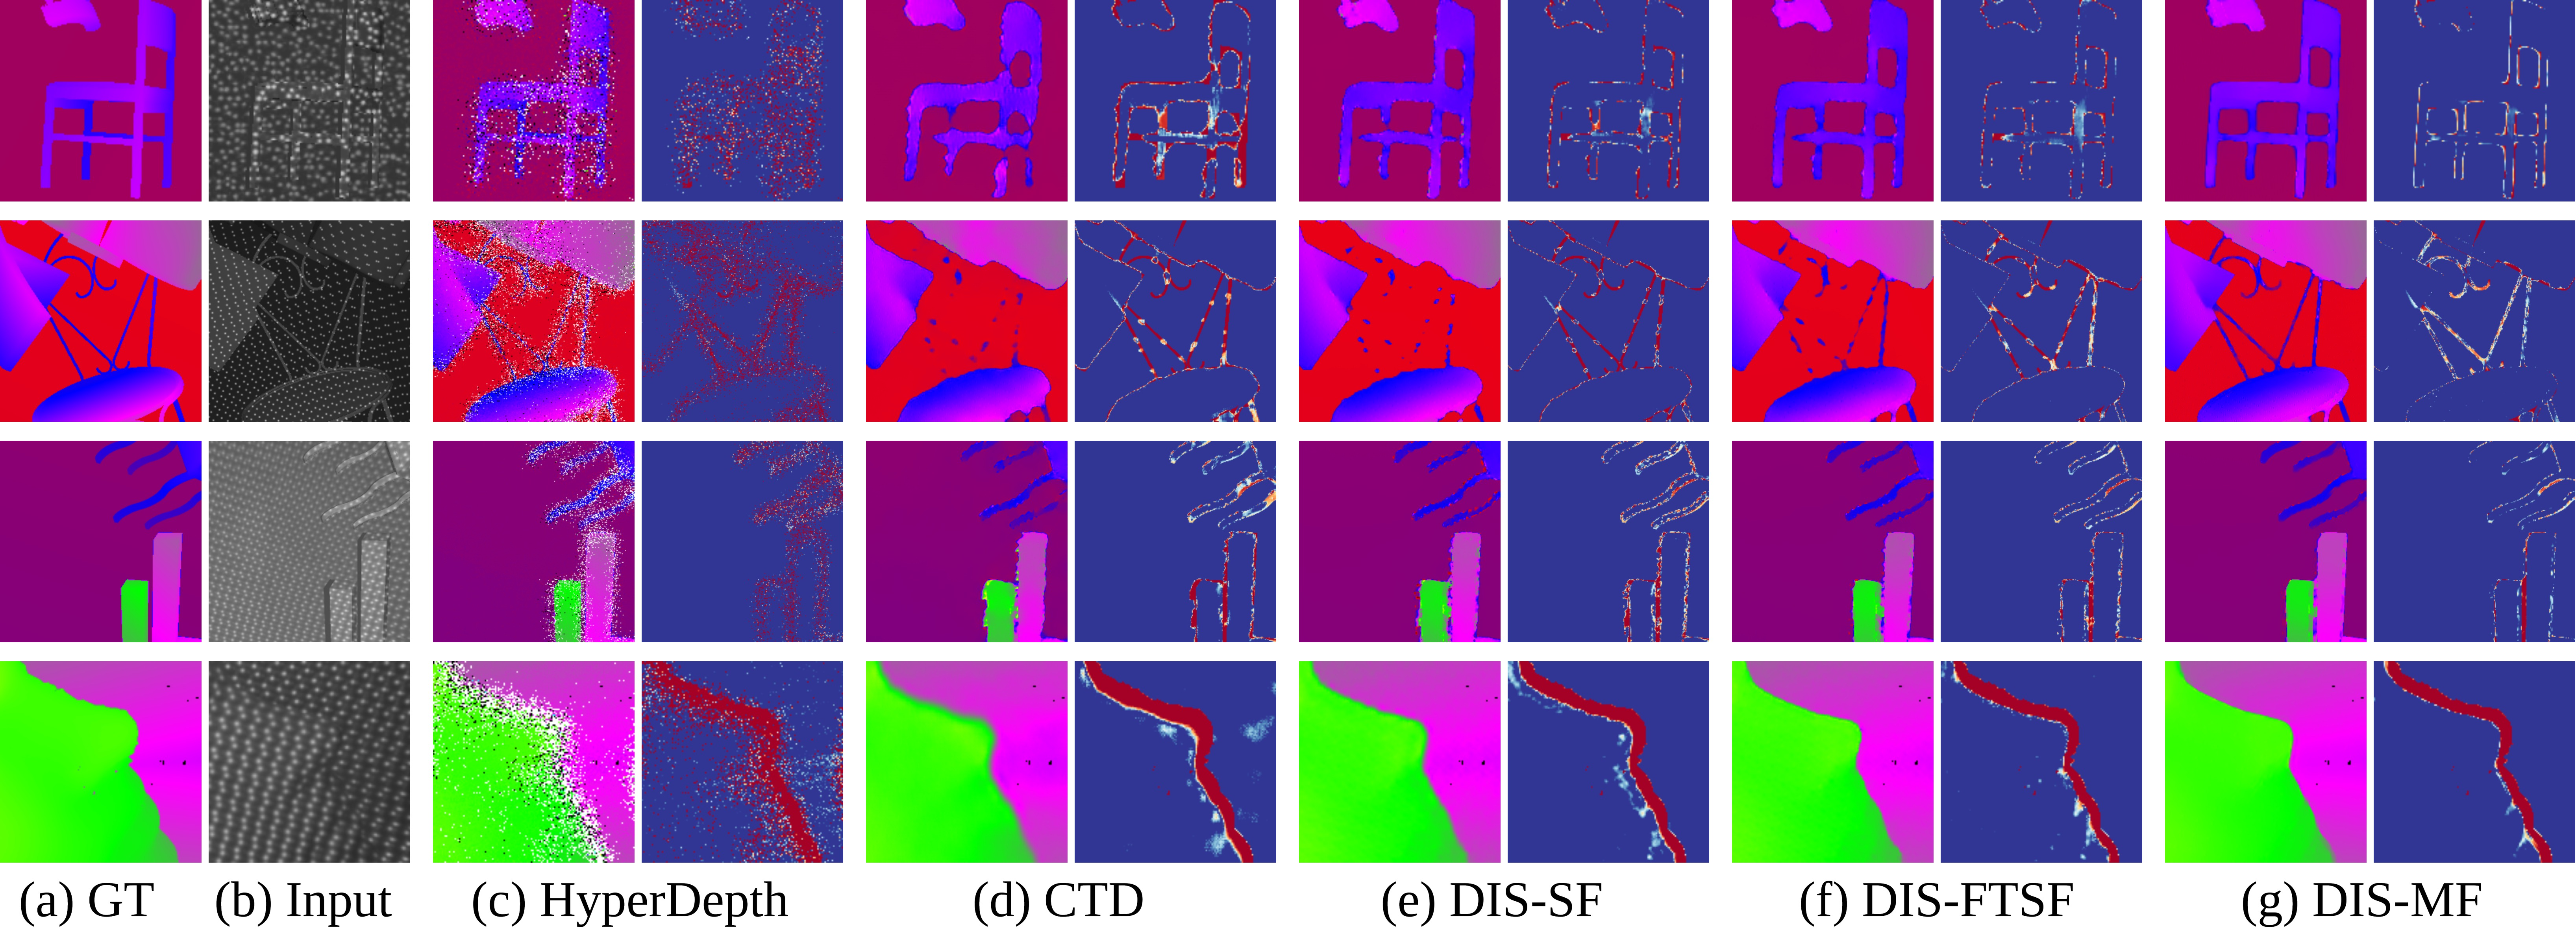
\includegraphics[width=1\linewidth]{images/chapter2/figures/Fig4.jpg}
    \end{center}
   \caption{Qualitative results of the methods and their corresponding error maps. (a)~Ground truth disparity map. (b)~Input dot image with projected pattern. (c)~HyperDepth~\cite{ryan2016hyperdepth}. (d)~CTD~\cite{riegler2019connecting}. (e)~Our DIS-SF model. (f)~Our DIS-FTSF model. (g)~Our DIS-MF Model. Each row represents a sample corresponding to each dataset in Table~\ref{table:c2_quantitative}. Points for which the ground truth data is unavailable are excluded from evaluation. For more sample images and extended qualitative evaluations, refer to the supplementary material.}
    \label{fig:c2_results}
\end{figure*}

\bigbreak\noindent\textbf{Metrics:} We use the percentage of outliers~$o(t)$ as in~\cite{riegler2019connecting} for quantitative evaluation, which is the percentage of pixels where the difference between the estimated and the ground truth disparities is greater than $t$.

\bigbreak\noindent\textbf{Comparison with existing methods:} We compare our models with Semi-Global Matching (SGM) algorithm~\cite{hirschmuller2007stereo}, HyperDepth~\cite{ryan2016hyperdepth}, and CTD~\cite{riegler2019connecting}. We observed through experiments that the window size of 13 for the SGM algorithm best suits our dataset. For HyperDepth, we used the same reimplementation code provided by~\cite{riegler2019connecting} with the hyperparameters that yield the best results in the original paper~\cite{ryan2016hyperdepth}. Since HyperDepth is a supervised method, we used the ground truth depth maps for training this model.

When training either CTD or our models on the real dataset, we use the pre-trained weights obtained from the synthetic data in order to speed up the training process. Moreover,  due to the limitations of the 3D scanner we used to capture ground truth, we had to put objects very close to the camera, resulting in very large values of disparities. Therefore, the statistics of disparities between the real dataset and the synthetic dataset are different, causing networks to get stuck in local minima when they are fine-tuned on the real data. We handled this issue by incorporating an additional loss function and using the SGM algorithm's valid outputs as pseudo-ground truth during the first few epochs of training. This loss function warms up the training process and resembles a coarse estimation of the ground truth at the beginning of the training. This stratagem prevents the networks from getting stuck in local minima and is used for both CTD and our models.

Qualitative comparison of the estimated disparities of the models on different datasets is depicted in Figure~\ref{fig:c2_results}. It is notable that all of our models produce sharper edges than the baseline model, CTD. Remarkably, our DIS-MF model best preserves the edges and is also capable of retaining high-resolution details. On the other hand, HyperDepth shows poor performance at discontinuities despite its accuracy in smooth regions. The figure also contrasts the quality of our DIS-SF and DIS-FTSF models and exhibits the usefulness of exploiting the DIS-MF model outputs to improve the accuracy of the DIS-SF model. Extended qualitative evaluations are provided in the supplementary material.

Table~\ref{table:c2_quantitative} provides the quantitative evaluation of the discussed models and shows the outcomes are consistent with the qualitative results. Table~\ref{table:c2_quantitative} also reflects the effect of the dot pattern on the performance of algorithms, where most models have the best accuracy in the experiment with the denser Kinect dot pattern. However, our models show robustness in all experiments. Particularly, DIS-MF yields overall the best results in all the experiments. Also, among the methods that predict disparities based on a single image, our DIS-FTSF model outperforms others overall.

For further experiments and ablation studies of the loss functions, validation masks, components of DIS-MF network, effect of imperfect disparities, utilized optical flow network, and extended qualitative analysis, refer to the supplementary material.

%-------------------------------------------------------------------------
\section{Conclusion}

We proposed DepthInSpace (DIS), which includes three self-supervised deep learning models to estimate depth from structured-light sensor data. Leveraging optical flow, we utilize information from multiple video frames from the same scene to improve depth estimation accuracy in three different self-supervised fashions. We qualitatively and quantitatively evaluated our models over four datasets: a publicly available synthetic dataset, two synthetic datasets customized with our setup parameters and dot pattern, and a real dataset that we made publicly available. The experiments validate the superiority of our models over the existing state-of-the-art methods.

The natural extension for future work will be on the one hand to apply our method to active stereo setup, combining the strengths of both sources of information, and on the other hand to deal with a simplified setup, for instance with a sparser less energy-hungry pattern of illumination.

\section{Supplementary Material}

\subsection{Notation Overview}

The notation in this section is consistent with the whole Chapter~\ref{sec:chapter2}. We name our loss functions as photometric loss~$\boldsymbol{\mathcal{L}_{ph}}$, smoothness loss~$\boldsymbol{\mathcal{L}_s}$, multi-view loss~$\boldsymbol{\mathcal{L}_{mv}}$, and pseudo-ground truth loss~$\boldsymbol{\mathcal{L}_{pgt}}$. For the DIS-MF model, we assume there are only two frames and we intend to merge Frame~$j$'s feature map~$\boldsymbol{\phi_j}$ into Frame~$i$'s feature map~$\boldsymbol{\phi_i}$. $\boldsymbol{X_i}$ represents 3D point cloud of Frame $i$ obtained using imperfect disparities and camera intrinsic parameters. We also define warped features~$\boldsymbol{\phi_{j \rightarrow i}}=w^{j \rightarrow i}(\boldsymbol{\phi_j})$, and warped points~$\boldsymbol{X_{j \rightarrow i}}=w^{j \rightarrow i}(\boldsymbol{X_j})$, where $w^{j \rightarrow i}(\cdot)$ stands for bilinear 2D warping via the optical flow $\boldsymbol{F_{i \rightarrow j}}$.

\subsection{Validation Binary Masks for the Multi-View Loss Function} \label{sec:c2_binary_masks}
As explained in the main paper, our multi-view loss function is defined as:
\begin{equation} \label{eqn:multi_view_loss}
    \boldsymbol{\mathcal{L}^{ij}_{mv}}=
    \bigg|
    \Big \langle \boldsymbol{X_{i}} -
    w^{j \rightarrow i}
    \big( \boldsymbol{T_{j \rightarrow i}} \times [\boldsymbol{X_{j}},\vec{\mathbf{1}}] \big) \Big \rangle_z
    \bigg| \times \boldsymbol{M'_{j \rightarrow i}}
\end{equation}
where $\boldsymbol{T_{j \rightarrow i}} \in \mathbb{R}^{3 \times 4}$ is the transformation matrix consisting of ego motion parameters, $\vec{\mathbf{1}}$ is an all one matrix, and $\langle\cdot\rangle_z$ operator returns the depth $z$ of its input 3D vector. In Equation~\ref{eqn:multi_view_loss}, $\boldsymbol{M'_{j \rightarrow i}}$ is a binary mask map validating warped points and preventing the network from being trained with noisy gradient information. In our DIS-SF model, two criteria must be met in order for a warped point to be indicated as valid. The first one is optical flow forward-backward consistency, suggested in \cite{zou2018df,meister2017unflow}:
\begin{equation}\label{eqn:supp_flow_forward_backward}
    \boldsymbol{M'_{FB}} = |\boldsymbol{F_{i \rightarrow j}} + w^{j \rightarrow i}(\boldsymbol{F_{j \rightarrow i}})|^2 < 0.01 \times (|\boldsymbol{F_{i \rightarrow j}}|^2 + |w^{j \rightarrow i}(\boldsymbol{F_{j \rightarrow i}})|^2) + 0.5
\end{equation}
which is exactly the binary mask map that is used in the fusion block of our DIS-MF model in the main paper. The second criterion excludes outlier points whose depths with respect to the camera position of the target frame has a considerable distance from the depths of their corresponding points in the target frame itself, \ie:
\begin{equation}
    \boldsymbol{M'_{O}} = \bigg|
    \Big \langle \boldsymbol{X_{i}} -
    w^{j \rightarrow i}
    \big( \boldsymbol{T_{j \rightarrow i}} \times [\boldsymbol{X_{j}},\vec{\mathbf{1}}] \big) \Big \rangle_z
    \bigg| < \tau
\end{equation}
where $\tau$ is a threshold set to 10 cm. Accordingly, the binary mask map in our DIS-SF model is defined as the intersection of these two criteria: $\boldsymbol{M'_{j \rightarrow i}} = \boldsymbol{M'_{FB}} \odot \boldsymbol{M'_{O}}$.

Instead, for the DIS-MF model, we define more strict and accurate criteria thanks to having access to imperfect disparities information. After checking optical flow forward-backward consistency in Equation~\ref{eqn:supp_flow_forward_backward}, we check if the optical flow is consistent with the rigid flow derived from camera motion parameters and imperfect disparities. Therefore, this constraint excludes pixels that either are warped with an erroneous optical flow or contain a significant error in their initially predicted depths:
\begin{equation}\label{eqn:flow_consistency}
    \boldsymbol{M'_{RF}} = \Big|\langle \boldsymbol{K} \times \boldsymbol{X_{i}}\rangle_{uv} - \big\langle w^{j \rightarrow i}
    (\boldsymbol{K} \times \boldsymbol{T_{j \rightarrow i}} \times [\boldsymbol{X_{j}},\vec{\mathbf{1}}])\big\rangle_{uv}   \Big| < 1
\end{equation}
where $\boldsymbol{K}$ is the camera intrinsic matrix, $\vec{\mathbf{1}}$ is an all one matrix, and $\langle\cdot\rangle_{uv}$ operator denotes mapping the 3D points on the image plane by dividing the operands by their depth components $z$. We map the points on the image plane because we are interested in taking into account the validity of the depth of the frame $\boldsymbol{z_j}$ independent of the depth of target frame $\boldsymbol{z_i}$. Thus, if a particular warped point has an accurate initially predicted depth to some degree, but the target point's depth is inaccurate, the warped point is still considered valuable for participating in the loss function, and in fact, it encourages the network to correct the depth of the target point. The threshold in Equation~\ref{eqn:flow_consistency} is set to 1, and it means that the warped point passes this criterion if it falls into its corresponding matched point's neighborhood of size one pixel on the target image plane.

Lastly, to prevent the network from being greedy in aggregating and fusing and also to encourage it to preserve sharp edges in the disparity map, we introduce another criterion that relates to the visual consistency of the warped and original normalized ambient images. This constraint specially excludes faulty warped points near the edges in the image and encourages the network to preserve the edges and geometry of the objects in the scene:
\begin{equation}\label{eqn:ambient_warp_check}
    \boldsymbol{M'_{VC}} = |\boldsymbol{A_{i}} - w^{j \rightarrow i}(\boldsymbol{A_{j}})|< 0.01
\end{equation}

This criterion is defined on the normalized ambient images, so the 0.01 threshold in Equation~\ref{eqn:ambient_warp_check} means points are accepted if their gray intensity levels differ less than one percent of the whole intensity level's range. Having these criteria together, we define the validation binary mask in our DIS-MF model as: $\boldsymbol{M'_{j \rightarrow i}} = \boldsymbol{M'_{FB}} \odot \boldsymbol{M'_{RF}} \odot \boldsymbol{M'_{VC}}$. An ablation study on the validation masks of DIS-MF is provided in Experiment~4 of Table~\ref{table:ablation_dis_mf} in Section~\ref{sec:c2_ablation_dis_mf}.

\subsection{Optical Flow Versus Back-Projection Projection Technique} \label{sec:c2_liteflownet}
As we briefly discussed in the main paper, while it is possible to find matched pixels using the back-projection projection technique, as it is used in CTD\cite{riegler2019connecting}, we opted for utilizing direct optical flow predictions for finding matched pixels among frames.

Optical flow provides us with two advantages. Firstly, the back-projection projection technique uses the momentary estimated depth and camera motion parameters to find matched pixels. As a result, the errors in the predicted depths propagate through the algorithm and degrade its performance. Also, it causes rapid fluctuations of the optimization landscape of the loss function. In contrast, we use a pre-trained optical flow network that finds matched pixels independently of the performance of depth estimation itself and provides a more reliable and stable loss function to optimize. Secondly, leveraging optical flow enables us to define strict binary masks (described in Section~\ref{sec:c2_binary_masks}) to exclude incorrectly warped pixels and only retain valuable data for supervising the training.

However, the drawback is that optical flow networks are designed to work with RGB images, while we provide them with ambient images that include only luminance information. To be more specific, we had to convert the ambient images to RGB format before feeding them to LiteFlowNet~\cite{hui2018liteflownet}. This conversion would degrade optical flow prediction performance, but it does not degrade the performance of our depth estimation models proportionately. The reason is that we have made our models robust to the performance of optical flow thanks to our multiple masking criteria (Section~\ref{sec:c2_binary_masks}). We only retain correctly warped pixels, so a lower optical flow performance results in fewer pixels for supervision, not more faulty pixels. An ablation study on the effect of the optical flow accuracy on our models' performances is provided in Section~\ref{sec:c2_ablation_gma}.

\subsection{Implementation Details} \label{sec:c2_implementation}

\noindent\textbf{Synthetic Datasets:} We use the renderer tool provided by~\cite{riegler2019connecting} to generate the synthetic datasets. Following their approach, we populate the scene with a subset of chair meshes from the ShapeNet Core dataset~\cite{shapenet2015} randomly scaled and rotated, placed at a distance between 0.5--3 m from the camera. A randomly slanted background plane at a distance between 2--5 m is also employed in the scene. Like~\cite{riegler2019connecting}, the camera is randomly translated within $20 \times 20 \times 20$ cm for capturing frames of each video sequence. However, we use our own camera's parameters to capture data from the scene. The baseline between our camera and projector is 2.46 cm, and the image resolution is $512 \times 432$ pixels. As we already mentioned in the main article, three different dot patterns are exploited in our experiments resulting in three synthetic datasets.

\bigbreak\noindent\textbf{Real Dataset:} We use an Artec Eva 3D scanner to scan 4 different 3D scenes containing various objects. The scanner has a few limitations, such as having limited depth range of 0.3--1.2 m and capturing only 100 depth frames per scan. For this reason, we take multiple partial scans of each scene and register them together using the point-to-plane variant of the ICP algorithm~\cite{rusinkiewicz2001efficient}, as mentioned in the main article. Once we obtain a 3D point cloud that covers the scene in a suitable way, the Ball-Pivoting algorithm~\cite{bernardini99ball} is applied to derive a 3D mesh of the scene. This mesh is used as ground truth. Subsequently, we scan each scene with our own structured-light sensor as to capture 148 pairs of dot images and ambient images. The sensor we use is equipped with a programmable switch, enabling the projector to be on and off, so it can capture dot images and ambient images alternately at the rate of 15 fps each. Given the capturing rate, each pair of dot image and ambient image captures the same scene approximately. We make use of these frames as 37 video sequences containing 4 frames each. As a result, 148 video sequences are obtained in total from all 4 scenes. Applying a block-matching technique on the dot images, we extract 148 depth images for each scene. The same ICP algorithm~\cite{rusinkiewicz2001efficient} is then used to align the depth images acquired using the sensor and the ground truth 3D mesh in order to obtain transformation matrices among the frames. We made the real dataset, along with the instructions to replicate the synthetic datasets, publicly available.

\bigbreak\noindent\textbf{Loss Functions:} Our proposed models' loss functions are explained in detail in the main paper. Here we clarify the coefficients used in the aggregate loss function. We introduced the aggregate loss function in the paper as:
\begin{multline}
     \shoveright{ \phantom{space space space space } \boldsymbol{\mathcal{L}} = \frac{1}{N}\sum_{i \in \Gamma} (\boldsymbol{\mathcal{L}^{i}_{ph}} + \lambda_{1}\boldsymbol{\mathcal{L}^{i}_{s}} + \lambda_{2}\boldsymbol{\mathcal{L}^{i}_{pgt}})
    + \frac{1}{N(N-1)}\sum_{i,j \in \Gamma} \lambda_{3}\boldsymbol{\mathcal{L}^{ij}_{mv}}}
    \label{eqn:aggregate_loss_supp}
\end{multline}
where $\Gamma$ denotes the image samples representing the same scene, $\boldsymbol{\mathcal{L}_{ph}}$ is the photometric loss, $\boldsymbol{\mathcal{L}_s}$ is the smoothness loss, $\boldsymbol{\mathcal{L}_{mv}}$ is the multi-view loss, and $\boldsymbol{\mathcal{L}_{pgt}}$ is the pseudo-ground truth loss. The coefficients in Equation~\eqref{eqn:aggregate_loss_supp} take different values for each model. These values are presented in Table~\ref{table:coef_supp}. As is shown in the table, the coefficient of the smoothness loss~$\lambda_{1}$ is set differently in our DIS-SF and DIS-MF models. Since our binary masks are less strict in DIS-SF, it allows more pixels in flat regions or backgrounds into $\boldsymbol{\mathcal{L}_{mv}}$. This promotes smoothness of depth maps, and accordingly, $\lambda_{1}$ is set to a smaller value in DIS-SF. In Section~\ref{sec:c2_ablation_hyperparams}, we provide detailed ablation study of searching for these hyperparameters.

\bigbreak\noindent\textbf{Training Details:} We have trained our models with a single NVIDIA Tesla V100 GPU. We exploit Adam~\cite{adam} optimizer with a learning rate of $10^{-4}$ for training. We set the batch size to 8 for training the DIS-SF and DIS-FTSF models and set it to 4 for the DIS-MF model due to GPU memory limitation.

Prior to training, we pre-save the outputs of LiteFlowNet~\cite{hui2018liteflownet} and provide them as the optical flow predictions to our model. Since there are 4 frames in each video sequence of our datasets, we need to pre-save 12 optical flow maps for each sequence. The reason is that we need both forward and backward optical flow data for each unique pair of frames in a video sequence.

We also pre-save the results of our DIS-SF model before training our DIS-MF model, and similarly, we pre-save the outputs of DIS-MF prior to training the DIS-FTSF model. These pre-saving steps make data preparation more convenient and result in an efficient training process. The time of training of our models, as well as the CTD~\cite{riegler2019connecting} model, on synthetic datasets and fine-tuning on the real dataset is presented in Table~\ref{table:train_time_supp}.

\begin{table}[t]
    \begin{center}
        \begin{tabular}{lccc}
        \hline
        Model & $\lambda_{1}$ & $\lambda_{2}$ & $\lambda_{3}$ \\
        \hline
        DIS-SF & 0.4 & 0.0 & 0.2 \\
        DIS-FTSF & 0.4 & 0.1 & 0.2 \\
        DIS-MF & 0.8 & 0.0 & 0.2 \\
        \hline
        \end{tabular}
    \end{center}
    \caption{The values of the coefficients used in our models' aggregate loss functions in Equation~\eqref{eqn:aggregate_loss_supp}. For ablation study of searching for these hyperparameters, refer to Section~\ref{sec:c2_ablation_hyperparams}}
    \label{table:coef_supp}
\end{table}

\begin{table}[b]
    \begin{center}
        \begin{tabular}{lcccc}
        \hline
        Dataset & CTD\cite{riegler2019connecting} & DIS-SF & DIS-FTSF & DIS-MF \\
        \hline
        Synthetic & 40 & 36 & 18 & 85 \\
        Real & 7 & 6 & 3 & 12\\
        \hline
        \end{tabular}
    \end{center}
    \caption{Approximate time (hours) of training/fine-tuning of the models on synthetic and real datasets with a single NVIDIA Tesla V100 GPU. Note that these reported times are measured assuming all required data are available. Therefore, the dependency of our models on each other's outputs should also be considered. For example, for obtaining a trained DIS-FTSF model on a synthetic dataset from scratch, we train the DIS-SF model for 36 hours, the DIS-MF model for 85 hours, and lastly, the DIS-FTSF model for 18 hours approximately.}
    \label{table:train_time_supp}
\end{table}

\subsection{Ablation Study} \label{sec:c2_ablation}
This section provides ablation studies regarding our introduced loss functions, setting hyperparameters, and design choices of our DIS-MF network architecture. All the experiments are evaluated on the synthetic dataset with the projection dot pattern from our industry partner.

\subsubsection{Efficacy of the Loss Functions} \label{sec:c2_ablation_loss}
Here, we attempt to distinguish the effectiveness of each of our individual loss functions. Table~\ref{table:ablation_dis_sf_loss} summarizes the quantitative evaluation of our DIS-SF network when it is trained with different combinations of loss functions. Since we use exactly the same network architecture of CTD~\cite{riegler2019connecting} in DIS-SF, it is also fair to compare the results with the case that the network is trained with loss functions employed in CTD. Furthermore, to show the generalization of the concept of fine-tuning with pseudo-labels, we fine-tuned the CTD model with our $\boldsymbol{\mathcal{L}_{pgt}}$ as an additional loss function and observed improvement in the outputs as it is indicated in Table~\ref{table:ablation_dis_sf_loss}. Lastly, we also examined the performance if we naively supervised the network with valid outputs resulting from the SGM algorithm~\cite{hirschmuller2007stereo}.

\begin{table}[t]
    \begin{center}
        \begin{tabular}{lcccc}
        \hline
        Loss & $o(0.5)$ & $o(1)$ & $o(2)$ & $o(5)$\\
        \hline
        Supervised by SGM Outputs & 21.1 & 15.9 & 12.0 & 7.91\\
        $\text{CTD Loss Functions}$ & 3.38 & 1.71 & 0.85 & 0.28\\
        $\text{CTD Loss Functions} + \boldsymbol{\mathcal{L}_{pgt}}$ & 2.62 & 1.25 & 0.58 & 0.14\\        
        $\boldsymbol{\mathcal{L}_{ph}}$ & 40.5 & 22.1 & 9.36 & 1.15\\
        $\boldsymbol{\mathcal{L}_{ph}} + \boldsymbol{\mathcal{L}_s}$ & 3.52 & 1.38 & 0.67 & 0.23\\
        $\boldsymbol{\mathcal{L}_{ph}} \phantom{IILL} + \boldsymbol{\mathcal{L}_{mv}}$ & 3.22 & 1.69 & 0.86 & 0.24\\
        $\boldsymbol{\mathcal{L}_{ph}} + \boldsymbol{\mathcal{L}_s} + \boldsymbol{\mathcal{L}_{mv}}$ & 2.31 & 1.24 & 0.62 & 0.19\\
        $\boldsymbol{\mathcal{L}_{ph}} + \boldsymbol{\mathcal{L}_s} + \boldsymbol{\mathcal{L}_{mv}} + \boldsymbol{\mathcal{L}_{pgt}}$ & \textbf{1.96} & \textbf{0.95} & \textbf{0.45} & \textbf{0.12}\\
        \hline
        \end{tabular}
    \end{center}

    \caption{Ablation study of individual loss terms: the photometric loss~$\boldsymbol{\mathcal{L}_{ph}}$, the smoothness loss~$\boldsymbol{\mathcal{L}_{s}}$, the multi-view loss~$\boldsymbol{\mathcal{L}_{mv}}$, and the pseudo-ground truth loss~$\boldsymbol{\mathcal{L}_{pgt}}$. Since we share the same network architecture for single-frame depth estimation with CTD~\cite{riegler2019connecting},  we could fairly contrast the superiority of our loss functions with respect to CTD's. The last row, which represents our DIS-FTSF model, yields overall the best results in terms of the percentage of outliers. Also, the effectiveness and generalizability of fine-tuning with pseudo-ground truth labels $\boldsymbol{\mathcal{L}_{pgt}}$ are shown when used for either fine-tuning our DIS-SF model or the CTD model.}
    \label{table:ablation_dis_sf_loss}
\end{table}

Figure~\ref{fig:c2_ablation_loss} also depicts some examples of our DIS-SF network outputs when it is trained with different combinations of loss functions. The samples demonstrate how our loss functions complement each other and form a robust depth estimation model altogether.

\begin{figure}[t]
    \begin{center}
        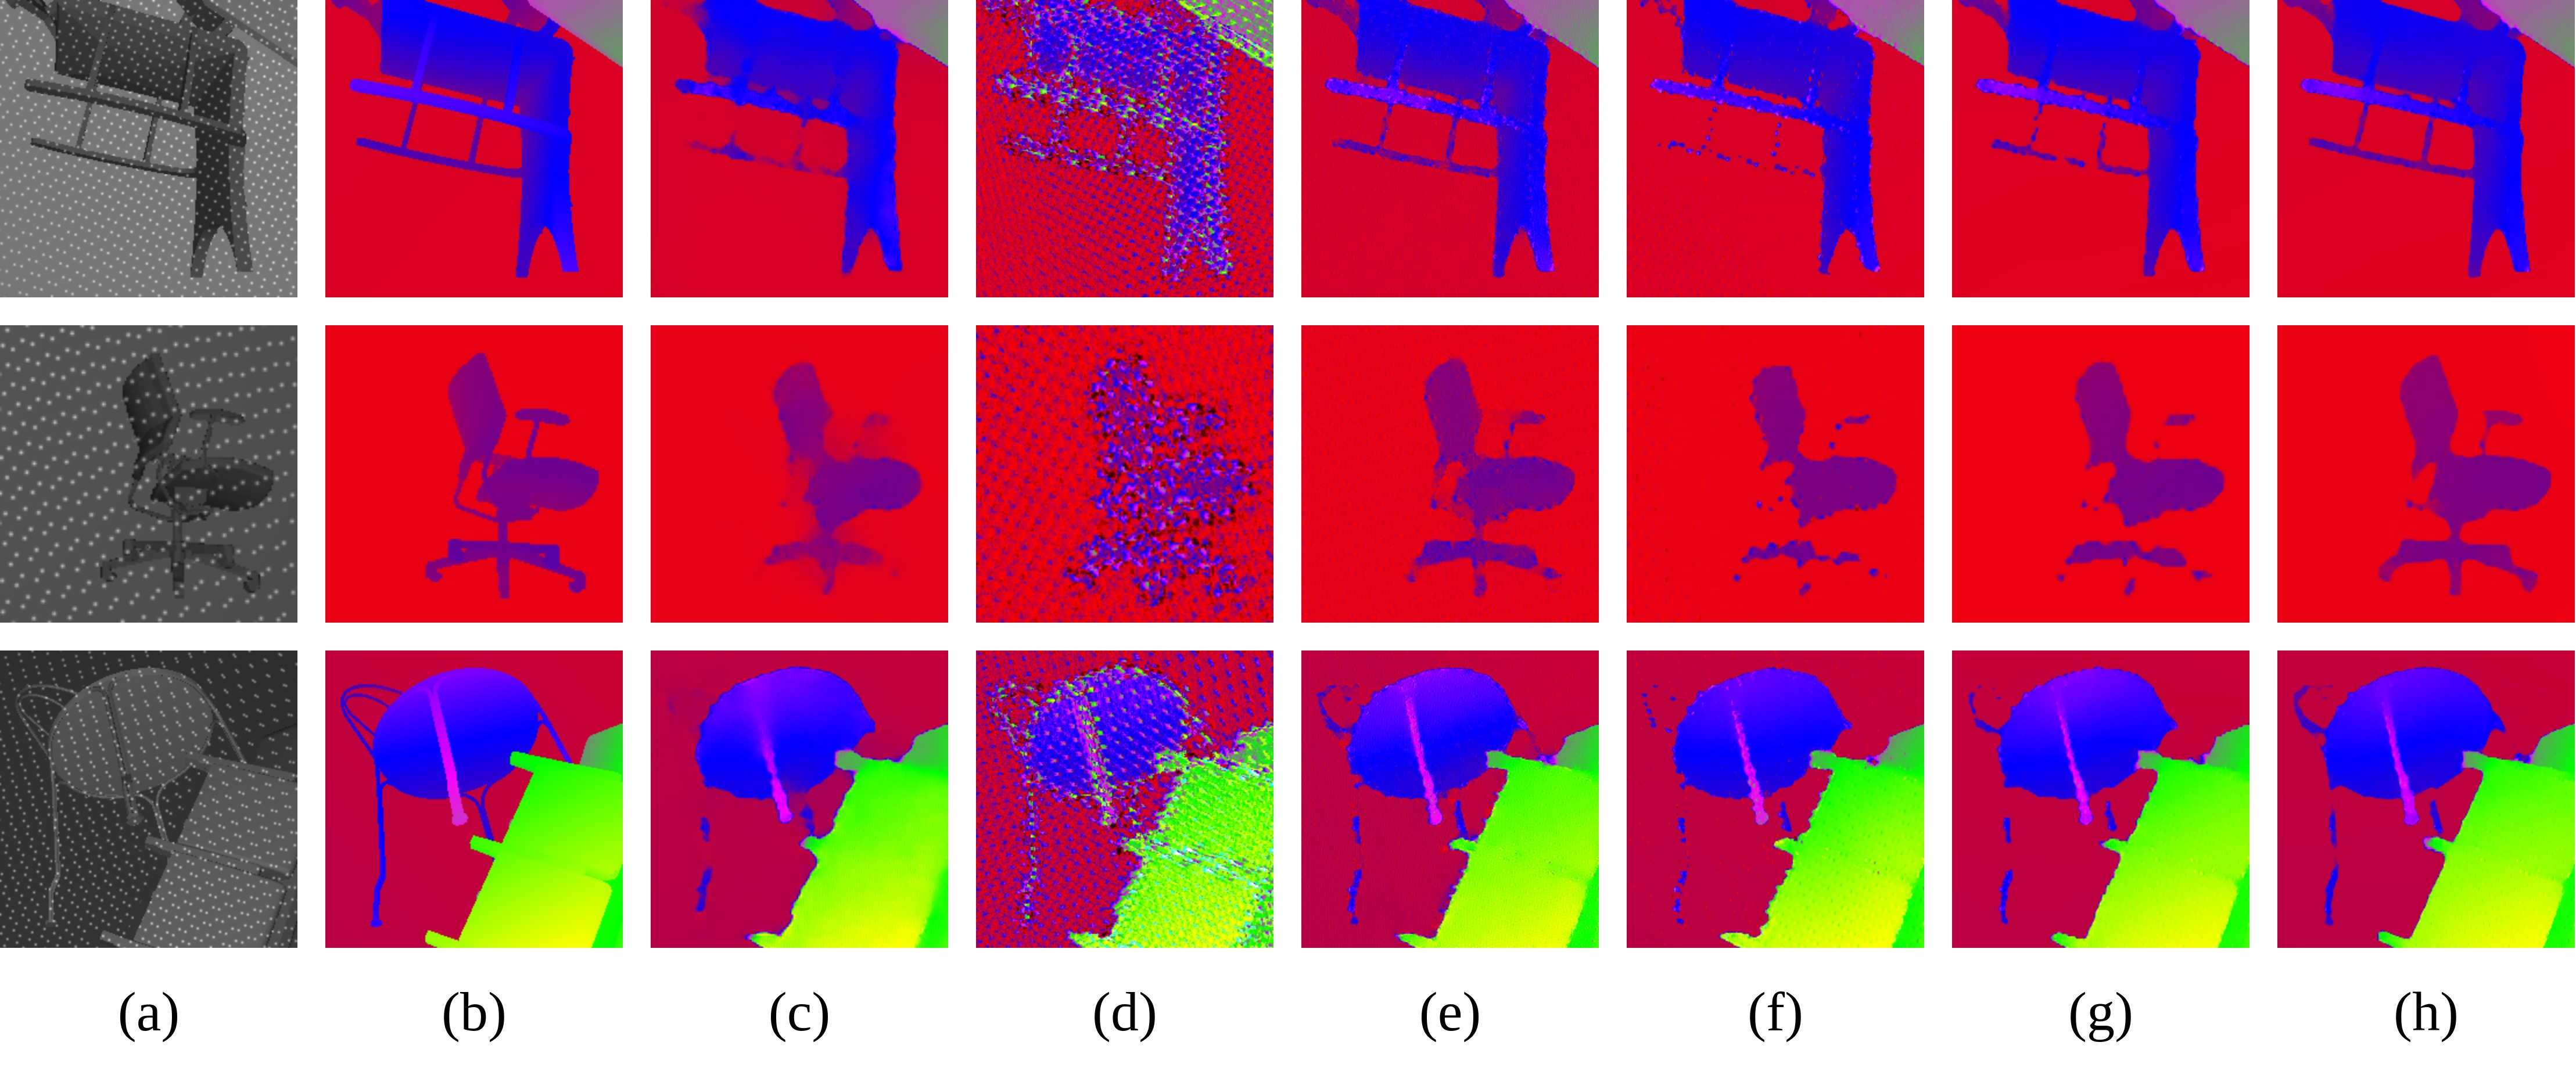
\includegraphics[width=1\linewidth]{images/chapter2/supp_figures/ablation_loss.jpg}
    \end{center}
   \caption{Qualitative ablation study of our individual loss functions. For each experiment, our DIS-SF network is trained with a different combination of our loss functions. (a)~Input dot image with projected pattern. (b)~Ground truth disparity map. (c)~Trained with CTD~\cite{riegler2019connecting} loss functions. (d)~Trained with $\boldsymbol{\mathcal{L}_{ph}}$. (e)~Trained with $\boldsymbol{\mathcal{L}_{ph}} + \boldsymbol{\mathcal{L}_s}$. (f)~Trained with $\boldsymbol{\mathcal{L}_{ph}} + \boldsymbol{\mathcal{L}_{mv}}$. (g)~Trained with $\boldsymbol{\mathcal{L}_{ph}} + \boldsymbol{\mathcal{L}_s} + \boldsymbol{\mathcal{L}_{mv}}$. (h)~Our final single-frame model trained with $\boldsymbol{\mathcal{L}_{ph}} + \boldsymbol{\mathcal{L}_s} + \boldsymbol{\mathcal{L}_{mv}} + \boldsymbol{\mathcal{L}_{pgt}}$.}
    \label{fig:c2_ablation_loss}
\end{figure}

\subsubsection{Searching for Hyperparameters} \label{sec:c2_ablation_hyperparams}
Table~\ref{table:ablation_hyperparams} represents the experiments we conducted for searching for the hyperparameters of our aggregate loss function for the DIS-SF and DIS-MF models. As we previously discussed, the hyperparameters should take different values due to the different mask criteria we defined in Section~\ref{sec:c2_binary_masks}. In the DIS-SF model, the mask criteria are less strict, and as a result, smoothness of disparity maps is inherently promoted in the multi-view loss~$\boldsymbol{\mathcal{L}_{mv}}$, whereas smoothness loss~$\boldsymbol{\mathcal{L}_{s}}$ in DIS-MF is emphasized directly. The experiments in Table~\ref{table:ablation_hyperparams} support this hypothesis.

\begin{table}[t]
    \begin{center}
        \begin{tabular}{c|cc|cccc}
        \hline
        Model & $\lambda_{1} (\boldsymbol{\mathcal{L}_s})$ & $\lambda_{3} (\boldsymbol{\mathcal{L}_{mv}})$ & $o(0.5)$ & $o(1)$ & $o(2)$ & $o(5)$ \\
        \hline
        \multirow{16}{75pt}{\centering DIS-SF} & 0.2 & 0.1 & 2.84 & 1.45 & 0.68 & 0.20 \\
        & 0.2 & 0.2 & 2.48 & 1.31 & 0.64 & 0.19 \\
        & 0.2 & 0.3 & 2.41 & 1.35 & 0.70 & 0.19 \\
        & 0.2 & 0.4 & 2.35 & 1.26 & 0.66 & 0.19 \\
        & 0.4 & 0.1 & 2.34 & 1.26 & 0.63 & 0.19 \\
        & 0.4 & 0.2 & \textbf{2.31} & \textbf{1.24} & \textbf{0.62} & \textbf{0.19} \\
        & 0.4 & 0.3 & 2.37 & 1.28 & 0.64 & 0.19 \\
        & 0.4 & 0.4 & 2.49 & 1.29 & 0.67 & 0.20 \\
        & 0.6 & 0.1 & 2.37 & 1.27 & 0.65 & 0.19 \\
        & 0.6 & 0.2 & 2.32 & 1.24 & 0.63 & 0.19 \\
        & 0.6 & 0.3 & 2.42 & 1.28 & 0.65 & 0.19 \\
        & 0.6 & 0.4 & 2.44 & 1.31 & 0.68 & 0.19 \\
        & 0.8 & 0.1 & 2.35 & 1.25 & 0.65 & 0.19 \\
        & 0.8 & 0.2 & 2.40 & 1.28 & 0.66 & 0.19 \\
        & 0.8 & 0.3 & 2.43 & 1.30 & 0.67 & 0.20 \\
        & 0.8 & 0.4 & 2.50 & 1.38 & 0.69 & 0.20 \\
        \hline
        \hline
        \multirow{15}{75pt}{\centering DIS-MF} & 0.2 & 0.1 & 2.19 & 0.93 & 0.43 & 0.12 \\
        & 0.2 & 0.2 & 1.98 & 0.93 & 0.44 & 0.12 \\
        & 0.2 & 0.3 & 1.99 & 0.96 & 0.47 & 0.13 \\
        & 0.4 & 0.1 & 1.92 & 0.86 & 0.39 & 0.11 \\
        & 0.4 & 0.2 & 1.87 & 0.84 & 0.39 & 0.11 \\
        & 0.4 & 0.3 & 1.81 & 0.88 & 0.42 & 0.11 \\
        & 0.6 & 0.1 & 2.06 & 0.86 & 0.36 & 0.10 \\
        & 0.6 & 0.2 & 1.97 & 0.84 & 0.37 & 0.10 \\
        & 0.6 & 0.3 & 1.70 & 0.80 & 0.38 & 0.11 \\
        & 0.8 & 0.1 & 1.96 & 0.82 & 0.35 & 0.10 \\
        & 0.8 & 0.2 & \textbf{1.58} & \textbf{0.71} & \textbf{0.32} & \textbf{0.10} \\
        & 0.8 & 0.3 & 1.66 & 0.77 & 0.36 & 0.10 \\
        & 1.0 & 0.1 & 1.88 & 0.75 & 0.34 & 0.10 \\
        & 1.0 & 0.2 & 1.72 & 0.75 & 0.34 & 0.10 \\
        & 1.0 & 0.3 & 1.62 & 0.76 & 0.35 & 0.10 \\
        \hline
        \end{tabular}
    \end{center}
    \caption{Ablation study of searching for hyperparameters of our aggregate loss function. It is noticeable that even poor choices of hyperparameters for the DIS-MF model still result in better performance than all experiments with the DIS-SF model. For further details on why separate experiments were needed for the DIS-SF and DIS-MF models, refer to Section~\ref{sec:c2_ablation_hyperparams} and \ref{sec:c2_implementation}.}
    \label{table:ablation_hyperparams}
\end{table}

\subsubsection{DIS-MF Network Architecture} \label{sec:c2_ablation_dis_mf}
The quantitative analysis of four experiments is presented in Table~\ref{table:ablation_dis_mf}: 1. Effect of the number of fused frames. 2. Effect of the number of fusion blocks and their channel size in the overall network architecture. 3. Efficacy of various processing elements in our DIS-MF network. 4. Contribution of validation binary masks, introduced in Section~\ref{sec:c2_binary_masks}, on our model's performance. Moreover, qualitative analysis of these four experiments are provided in Figures~\ref{fig:c2_ablation_mf_n}, \ref{fig:c2_ablation_mf_blch}, \ref{fig:c2_ablation_mf_2d3d}, and \ref{fig:c2_ablation_mf_masks}.

In particular, it is notable that despite the hugeness of our network and its robustness against variation of the number of fusion blocks or their channel size, according to Table~\ref{table:ablation_dis_mf}, the performance still degrades when we remove continuous 3D convolution and perform fusion only on the 2D grid map. As also discussed in the main paper, in the context of depth estimation from conventional RGB camera, works like DeepV2D~\cite{teed2019deepv2d}, DeepMVS~\cite{huang2018deepmvs}, DeepSFM~\cite{wei2020deepsfm}, and DPSNet~\cite{im2018dpsnet} attempt to fuse information of multiple frames on the 2D grid. We cannot directly compare our work with them because they are designed to operate on RGB images. Still, we attempt to demonstrate how leveraging fusion both on the 2D grid and in the 3D space improves the performance in the structured-light setup depth estimation.

Lastly, Figure~\ref{fig:c2_visualize_masks} exemplifies the behavior of each binary mask criterion in Section~\ref{sec:c2_binary_masks} and shows how these masks exclude low confidence pixels and prevent them from supervising the training.



\begin{table}[t]

\rotatebox{90}{
\begin{minipage}{0.99\textheight}

\begin{center}
        \begin{tabular}{c|cc|ccc|ccc|cccc|c}
        \hline
        \multirow{2}{*}{$\boldsymbol{N}$} & \multicolumn{2}{c|}{Fusion Blocks} & \multicolumn{3}{c|}{Network Components} & \multicolumn{3}{c|}{Binary Masks Criteria} & \multicolumn{4}{c|}{Metrics [\%]} &
        \multirow{2}{*}{Examples}\\
        & \small Num. & \small Ch. & \small 2D Fus. & \small 3D Fus. & \small Ref. & \small $\boldsymbol{M'_{FB}}$ & \small $\boldsymbol{M'_{RF}}$ & \small $\boldsymbol{M'_{VC}}$ & $o(0.5)$ & $o(1)$ & $o(2)$ & $o(5)$ \\
        \hline
        \noalign{\vskip 0.25mm}    
        \multicolumn{14}{l}{\small Experiment 1: Effect of the number of fused frames~$\boldsymbol{N}$.} \\
        \hline
        % Number of frames experiments
        2 & 4 & 32 & $\bullet$ & $\bullet$ & $\bullet$ & $\bullet$ & $\bullet$ & $\bullet$ & 1.90 & 0.83 & 0.37 & 0.10 & Fig. \ref{fig:c2_ablation_mf_n}.c \\
        3 & 4 & 32 & $\bullet$ & $\bullet$ & $\bullet$ & $\bullet$ & $\bullet$ & $\bullet$ & 1.73 & 0.75 & 0.34 & 0.10 & Fig. \ref{fig:c2_ablation_mf_n}.d \\
        4 & 4 & 32 & $\bullet$ & $\bullet$ & $\bullet$ & $\bullet$ & $\bullet$ & $\bullet$ & \textbf{1.58} & \textbf{0.71} & \textbf{0.32} & \textbf{0.10} & Fig. \ref{fig:c2_ablation_mf_n}.e \\
        \hline
        \noalign{\vskip 0.25mm}
        \multicolumn{14}{l}{\small Experiment 2: Effect of the number of fusion blocks and their channel size.} \\        
        \hline
        % Fusion blocks experiments
        4 & 2 & 48 & $\bullet$ & $\bullet$ & $\bullet$ & $\bullet$ & $\bullet$ & $\bullet$ & 1.59 & 0.72 & 0.33 & 0.10 & Fig. \ref{fig:c2_ablation_mf_blch}.c \\
        4 & 4 & 32 & $\bullet$ & $\bullet$ & $\bullet$ & $\bullet$ & $\bullet$ & $\bullet$ & \textbf{1.58} & \textbf{0.71} & \textbf{0.32} & \textbf{0.10} & Fig. \ref{fig:c2_ablation_mf_blch}.d \\
        4 & 6 & 24 & $\bullet$ & $\bullet$ & $\bullet$ & $\bullet$ & $\bullet$ & $\bullet$ & 1.62 & 0.72 & 0.33 & 0.10 & Fig. \ref{fig:c2_ablation_mf_blch}.e \\
        4 & 8 & 16 & $\bullet$ & $\bullet$ & $\bullet$ & $\bullet$ & $\bullet$ & $\bullet$ & 1.60 & 0.73 & 0.33 & 0.10 & Fig. \ref{fig:c2_ablation_mf_blch}.f \\
        \hline
        \noalign{\vskip 0.25mm}
        \multicolumn{14}{l}{\small Experiment 3: Each processing component's efficacy in the network architecture.} \\      
        \hline
        % Network components experiments
        4 & 4 & 32 & $\circ$ & $\bullet$ & $\bullet$ & $\bullet$ & $\bullet$ & $\bullet$ & 1.58 & 0.72 & 0.33 & 0.10 & Fig. \ref{fig:c2_ablation_mf_2d3d}.c \\
        4 & 4 & 32 & $\bullet$ & $\circ$ & $\bullet$ & $\bullet$ & $\bullet$ & $\bullet$ & 1.74 & 0.74 & 0.34 & 0.11 & Fig. \ref{fig:c2_ablation_mf_2d3d}.d \\
        4 & 4 & 32 & $\bullet$ & $\bullet$ & $\circ$ & $\bullet$ & $\bullet$ & $\bullet$ & 1.98 & 1.04 & 0.50 & 0.13 & Fig. \ref{fig:c2_ablation_mf_2d3d}.e \\
        4 & 4 & 32 & $\bullet$ & $\bullet$ & $\bullet$ & $\bullet$ & $\bullet$ & $\bullet$ & \textbf{1.58} & \textbf{0.71} & \textbf{0.32} & \textbf{0.10} & Fig. \ref{fig:c2_ablation_mf_2d3d}.f \\
        \hline
        \noalign{\vskip 0.25mm}
        \multicolumn{14}{l}{\small Experiment 4: Impact of the validation binary masks on the performance.} \\
        \hline
        % Masks experiments
        4 & 4 & 32 & $\bullet$ & $\bullet$ & $\bullet$ & $\bullet$ & $\circ$ & $\circ$ & 2.19 & 1.11 & 0.53 & 0.14 & Fig. \ref{fig:c2_ablation_mf_masks}.c \\
        4 & 4 & 32 & $\bullet$ & $\bullet$ & $\bullet$ & $\bullet$ & $\circ$ & $\bullet$ & 1.63 & 0.71 & 0.33 & 0.10 & Fig. \ref{fig:c2_ablation_mf_masks}.d \\
        4 & 4 & 32 & $\bullet$ & $\bullet$ & $\bullet$ & $\bullet$ & $\bullet$ & $\circ$ & 1.88 & 0.91 & 0.42 & 0.11 & Fig. \ref{fig:c2_ablation_mf_masks}.e \\
        4 & 4 & 32 & $\bullet$ & $\bullet$ & $\bullet$ & $\bullet$ & $\bullet$ & $\bullet$ & \textbf{1.58} & \textbf{0.71} & \textbf{0.32} & \textbf{0.10} & Fig. \ref{fig:c2_ablation_mf_masks}.f \\
        \hline
        \end{tabular}
    \end{center}
    \vspace{-4ex}
    \caption{\small Ablation study of DIS-MF network. This table summarizes four experiments, in each of which the effect of a subset of particular design choices is examined independently. Firstly, this study shows how the performance of DIS-MF improves with higher numbers of fused frames~$\boldsymbol{N}$. The second experiment examines how many cascaded fusion blocks and with which channel size lead to better results. The channel size and the number of blocks are selected such that computation resources become comparable. As the results suggest, our proposed architecture is robust against variations of these parameters. The third experiment evaluates the efficacy of processing components in our network architecture. Our fusion block contains aggregating convolution modules both on the 2D grid map and in the continuous 3D space. Here, the contribution of each part to the final performance is shown (\eg, the $o(0.5)$ metric deteriorates from \textbf{1.58} \% to \textbf{1.74} \% when we perform aggregation only on the 2D grid map). For further details on why this comparison is important, please refer to Section~\ref{sec:c2_ablation_dis_mf}. Also, the effectiveness of the refinement structure in the post-processing part of our network architecture is investigated in this experiment. Lastly, this study demonstrates how each of the binary mask criteria in Section~\ref{sec:c2_binary_masks} affects our DIS-MF model's performance in the fourth experiment. Qualitative analyses corresponding to each of these experiments are provided in Figures~\ref{fig:c2_ablation_mf_n}, \ref{fig:c2_ablation_mf_blch}, \ref{fig:c2_ablation_mf_2d3d}, and \ref{fig:c2_ablation_mf_masks}.}
    \label{table:ablation_dis_mf}

\end{minipage}}

\end{table}


\begin{figure*}[t] 
    \begin{center}
        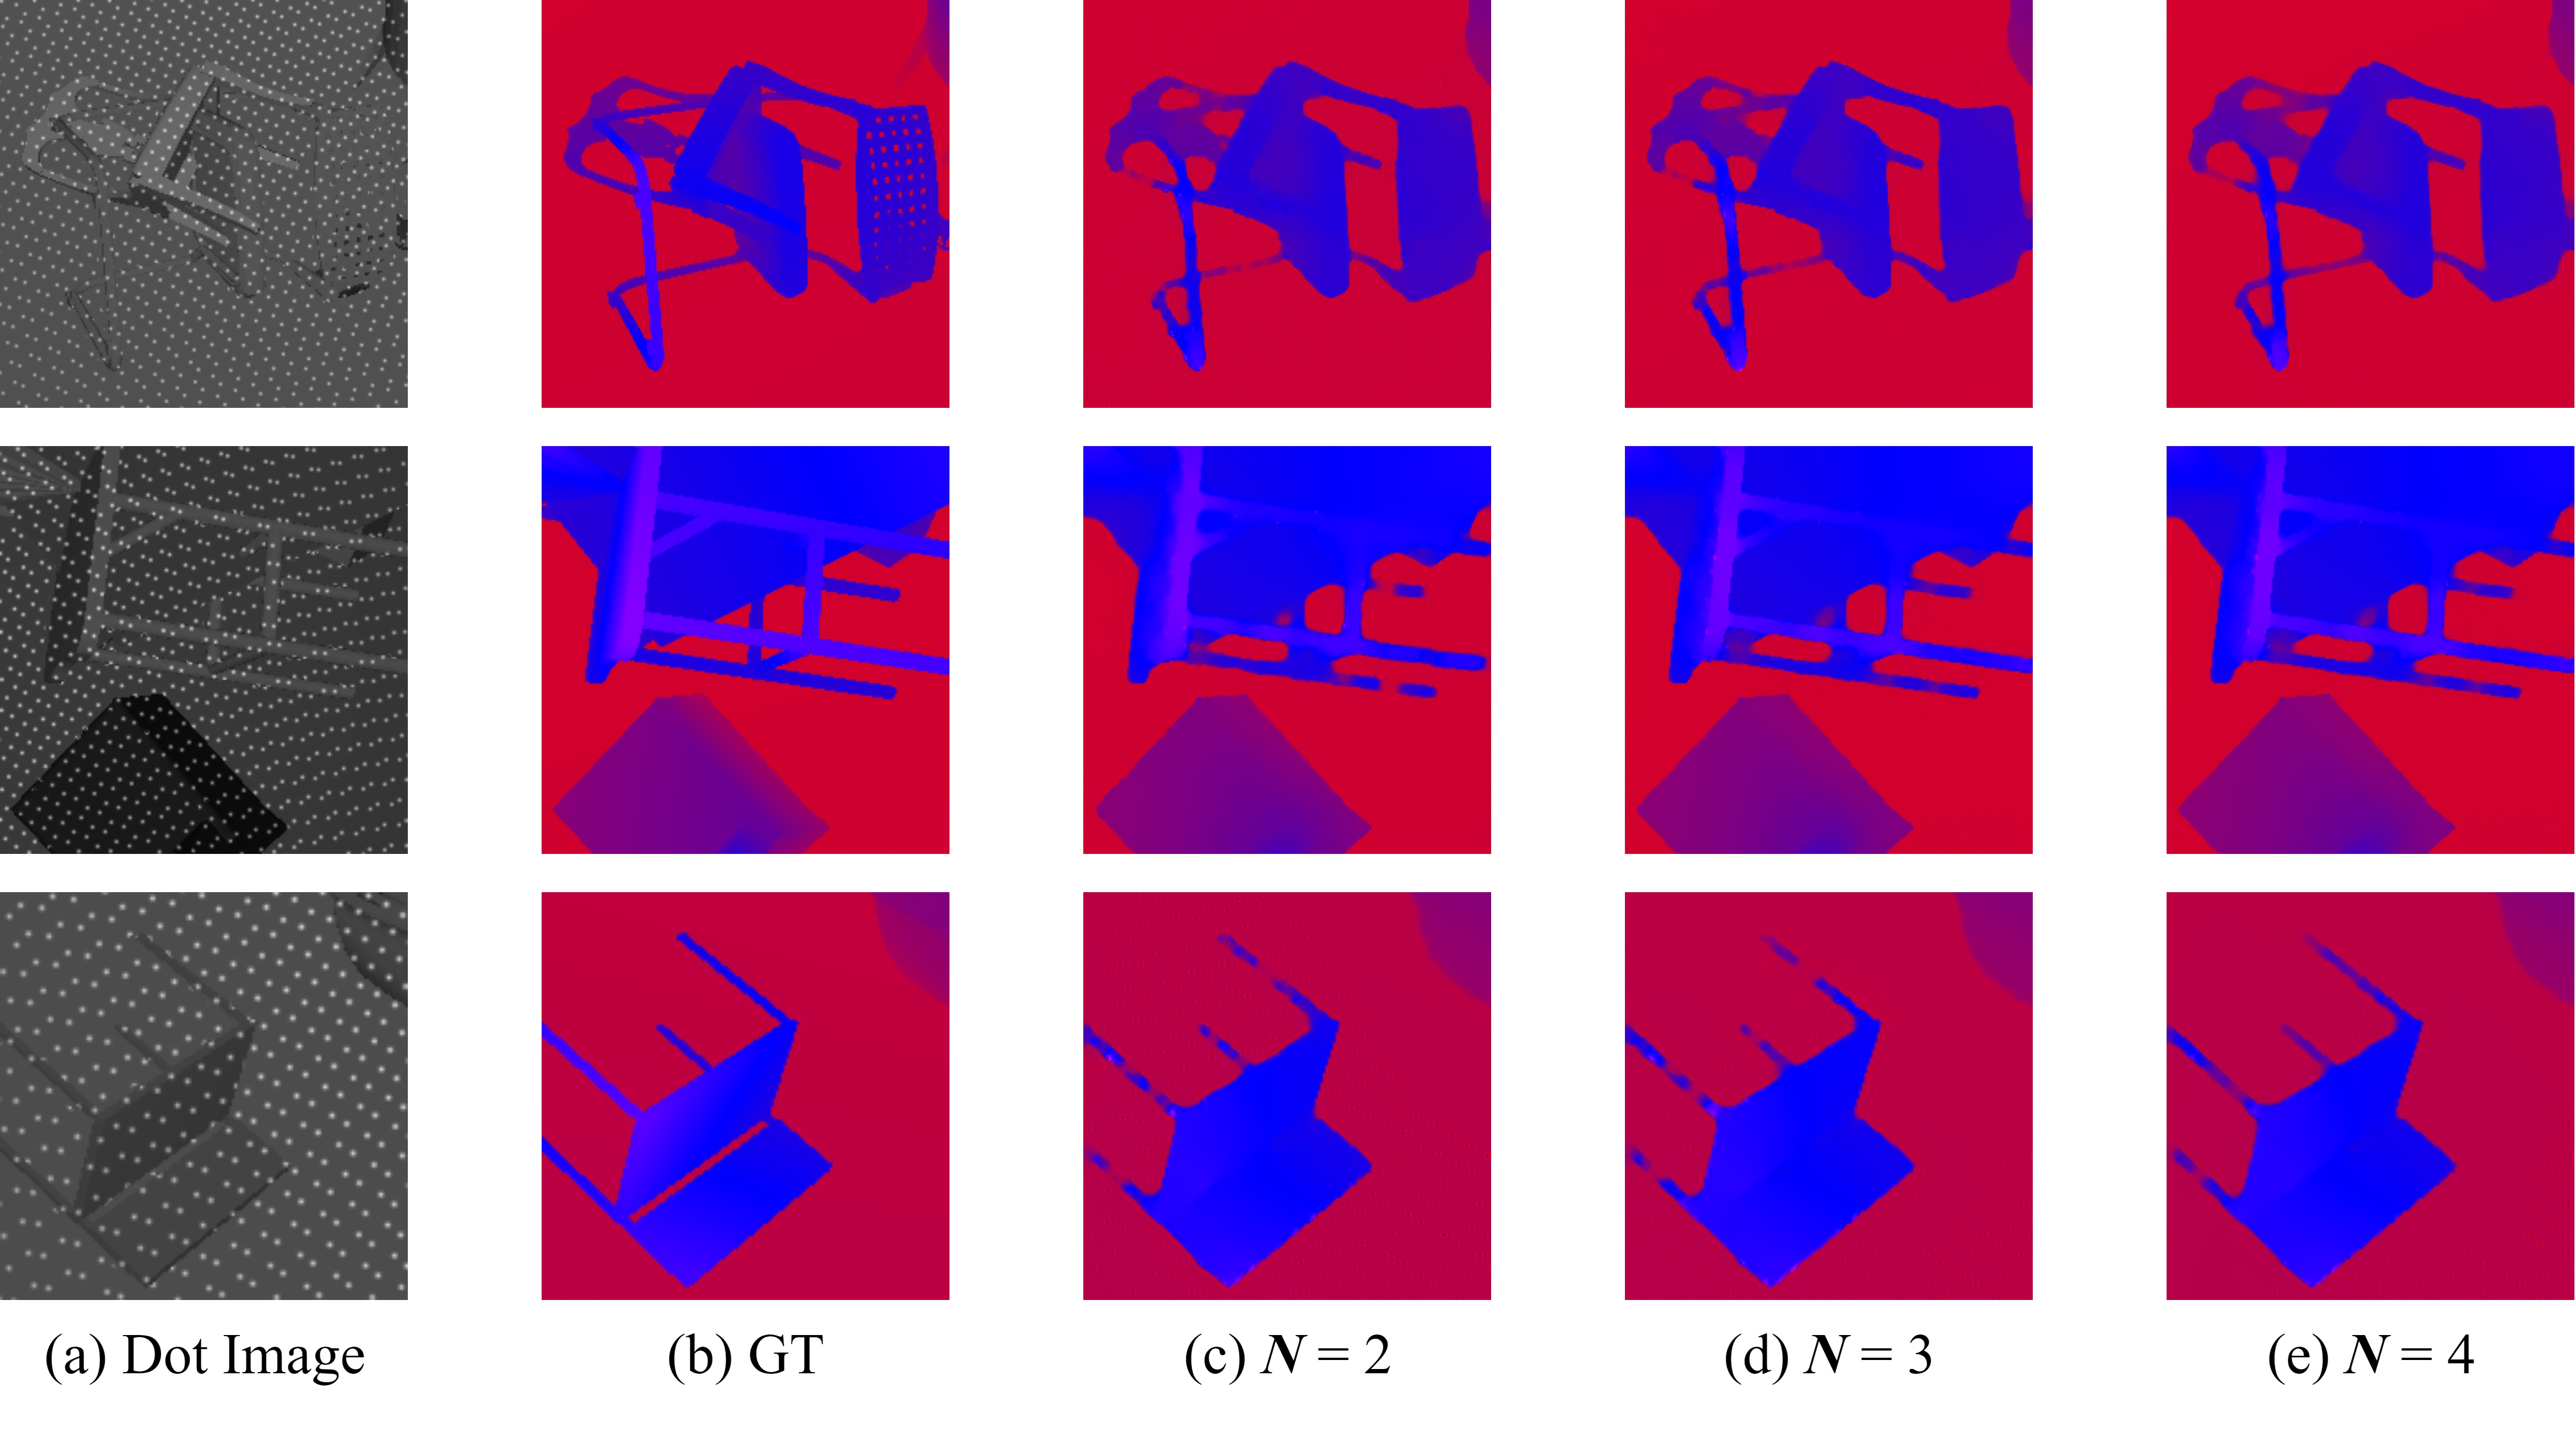
\includegraphics[width=1.0\linewidth]{images/chapter2/supp_figures/ablation_mf_n.jpg}
    \end{center}
   \caption{Qualitative analysis of Experiment 1 in Table~\ref{table:ablation_dis_mf}, where we examine the effect of the number of fused frame~$\boldsymbol{N}$ on DIS-MF performance. (a)~Input dot image. (b)~Ground truth disparity map. (c)~DIS-MF's output with $\boldsymbol{N} = 2$. (d)~DIS-MF's output with $\boldsymbol{N} = 3$. (e)~DIS-MF's output with $\boldsymbol{N} = 4$. As expected according to Table~\ref{table:ablation_dis_mf}, DIS-MF performs better at completing disparity maps as the number of fused frames increases.} \label{fig:c2_ablation_mf_n}
\end{figure*}

\begin{figure}[t]
    \begin{center}
        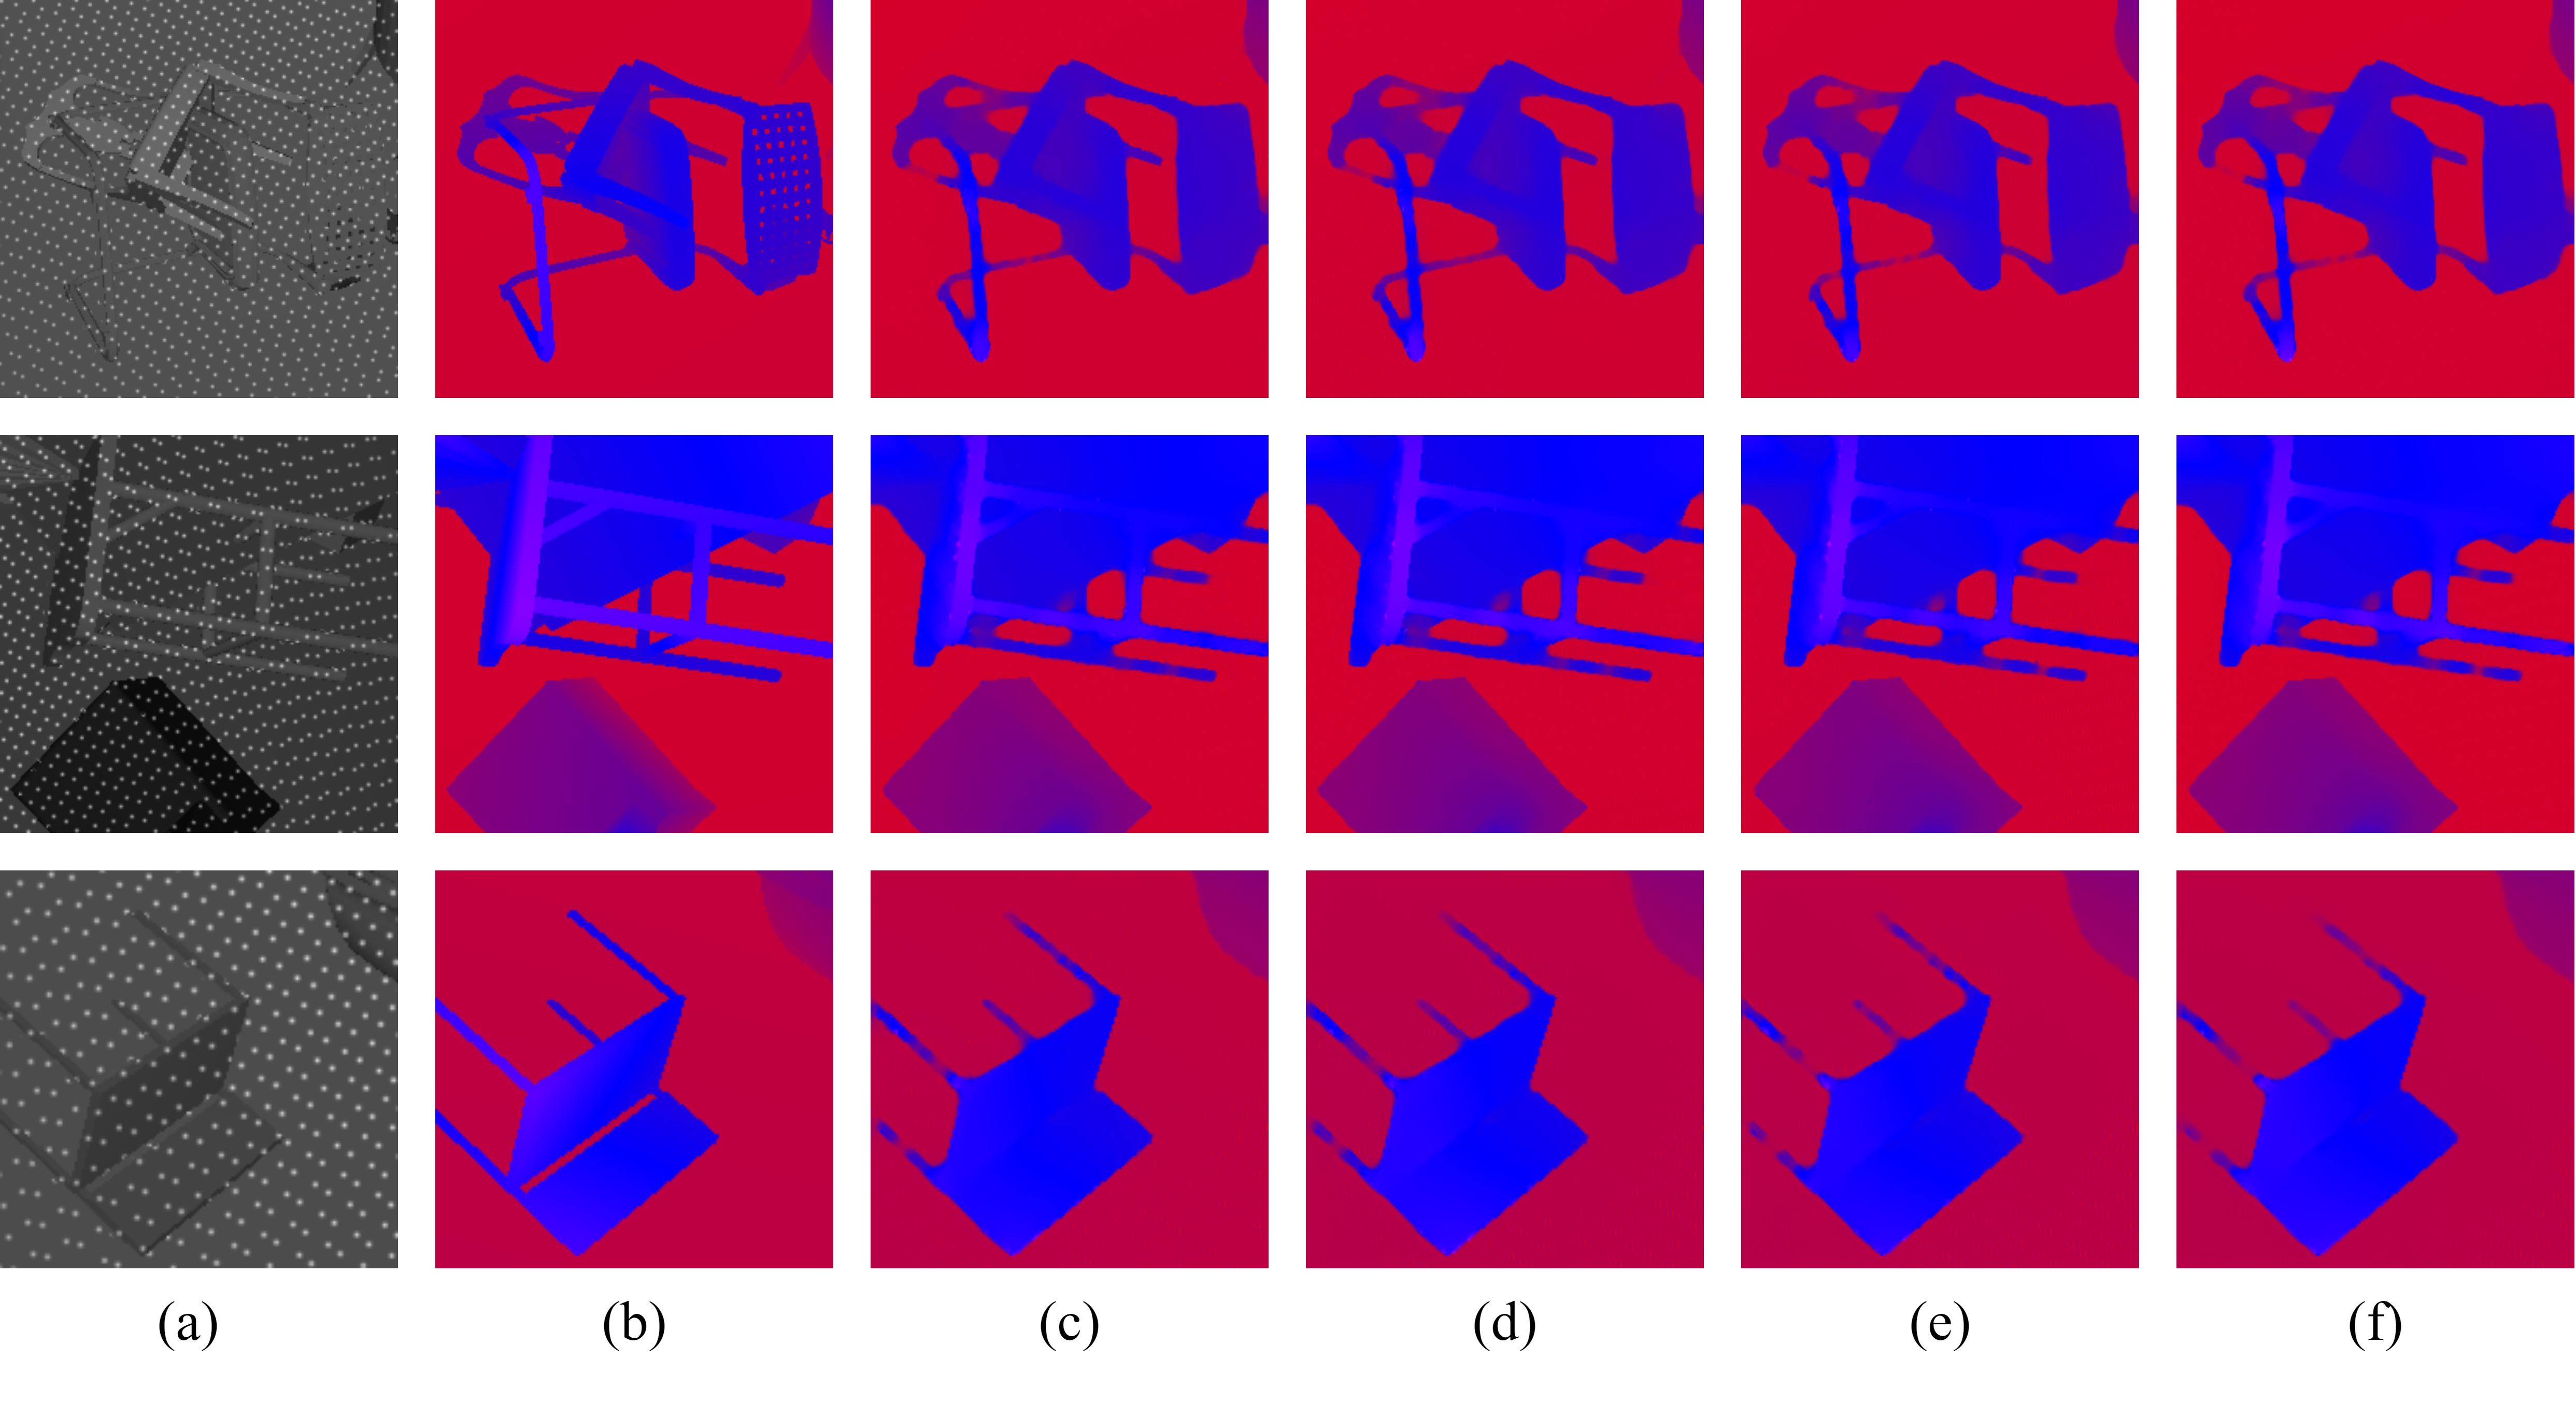
\includegraphics[width=1.0\linewidth]{images/chapter2/supp_figures/ablation_mf_blch.jpg}
    \end{center}
   \caption{Qualitative analysis of Experiment 2 in Table~\ref{table:ablation_dis_mf}, where we examine the effect of the number of fusion blocks and their channel size on DIS-MF performance (The architecture is presented in Figure 3 in the main paper). (a)~Input dot image. (b)~Ground truth disparity map. (c)~DIS-MF's output with 2 cascaded fusion blocks, each of which with 48 channels. (d)~DIS-MF's output with 4 cascaded fusion blocks, each of which with 32 channels. (e)~DIS-MF's output with 6 cascaded fusion blocks, each of which with 24 channels. (f)~DIS-MF's output with 8 cascaded fusion blocks, each of which with 16 channels. As expected according to Table~\ref{table:ablation_dis_mf}, DIS-MF performs robustly with different choices of parameters, and having 4 fusion blocks with 32 channels produces higher quality disparity maps.}
    \label{fig:c2_ablation_mf_blch}
\end{figure}

\begin{figure}[t]
    \begin{center}
        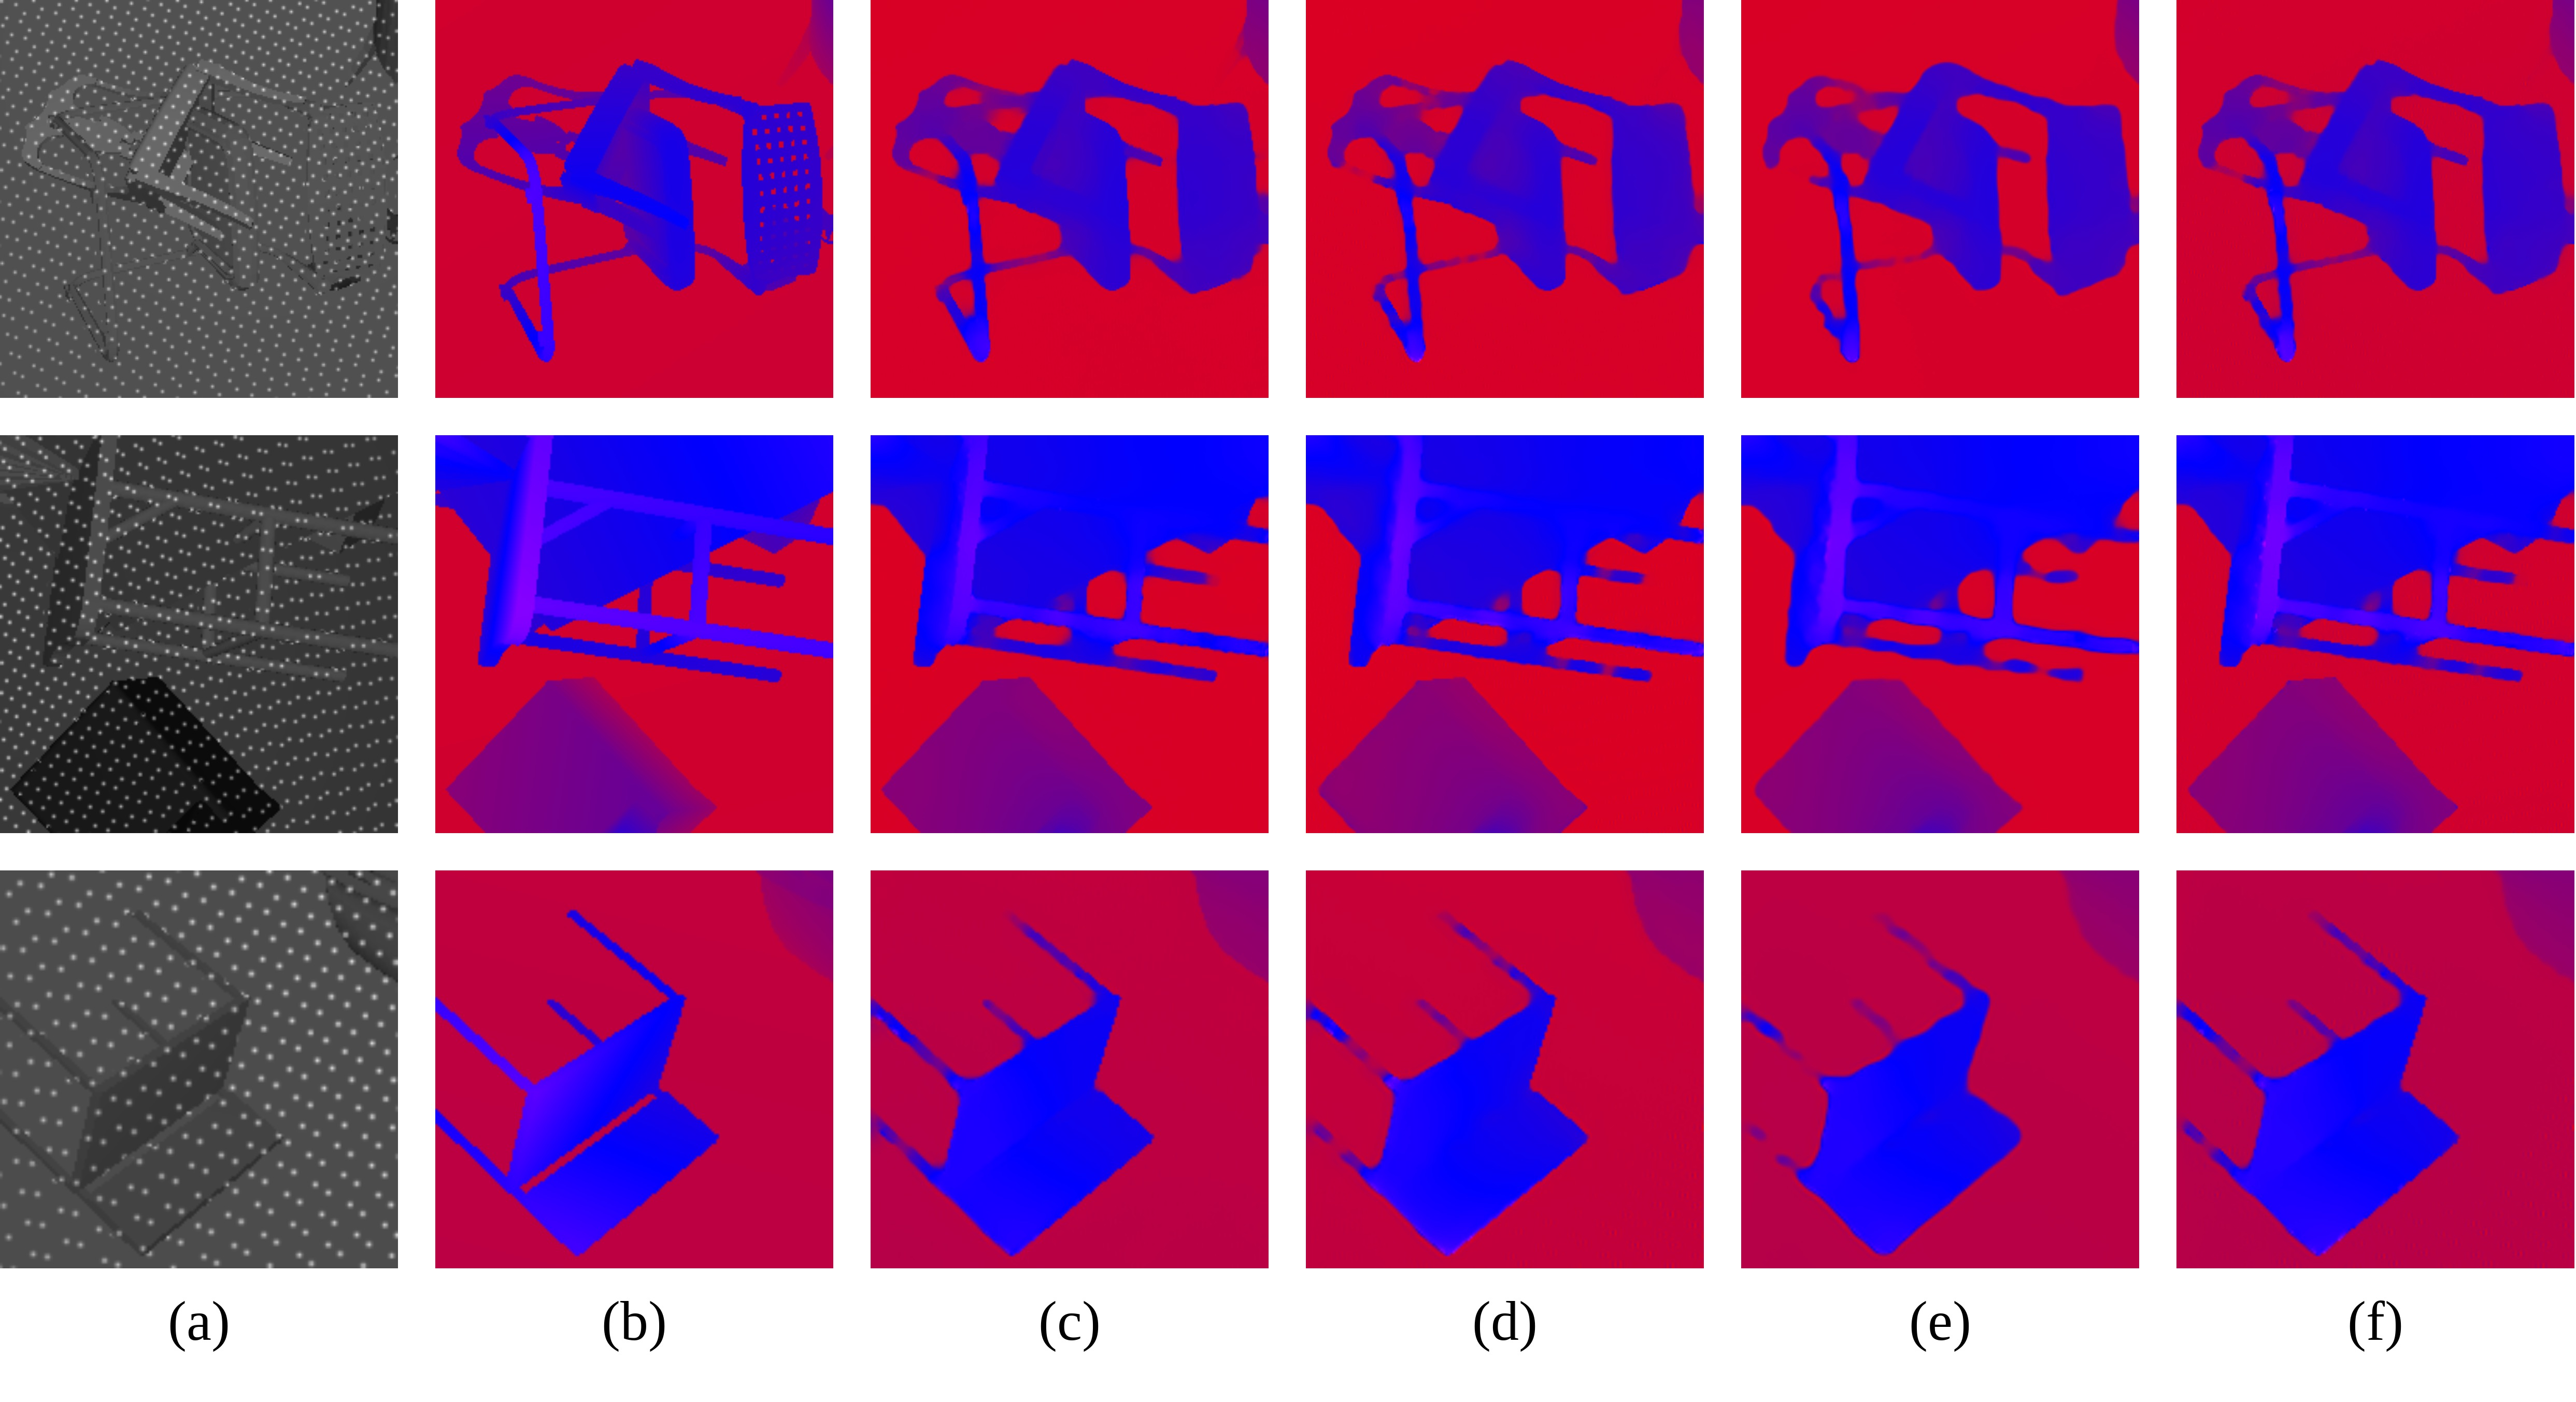
\includegraphics[width=1.0\linewidth]{images/chapter2/supp_figures/ablation_mf_2d3d.jpg}
    \end{center}
   \caption{Qualitative analysis of Experiment 3 in Table~\ref{table:ablation_dis_mf}, where we examine the efficacy of each processing component on DIS-MF performance (Components are introduced in Section 3.2 in the main paper). (a)~Input dot image. (b)~Ground truth disparity map. (c)~DIS-MF's output when fusion is done only in the continuous 3D space. (d)~DIS-MF's output when fusion is done only on the 2D grid map. (e)~DIS-MF's output when the refinement structure (post-processing part in Figure 3 in the main paper) is removed from the network architecture. (f)~DIS-MF's output with all processing components. This figure, in particular, contrasts the capability of DIS-MF in completing disparity maps when fusion is performed in the continuous 3D space versus when it is done on the 2D grid map. Additionally, by comparing columns (c) and (f), one observes that fusing only in the 3D space results in fewer missing points compared to having both 2D and 3D fusion in the architecture. However, the edge fattening artifact, which is inherent to continuous 3D convolution, is more pronounced in the disparity maps generated by aggregating data only in the 3D space. Overall, employing both 2D and 3D fusion components produces balanced disparity maps concerning completing missing points and preserving edges and discontinuities in the disparity maps.}
    \label{fig:c2_ablation_mf_2d3d}
\end{figure}

\begin{figure}[t]
    \begin{center}
        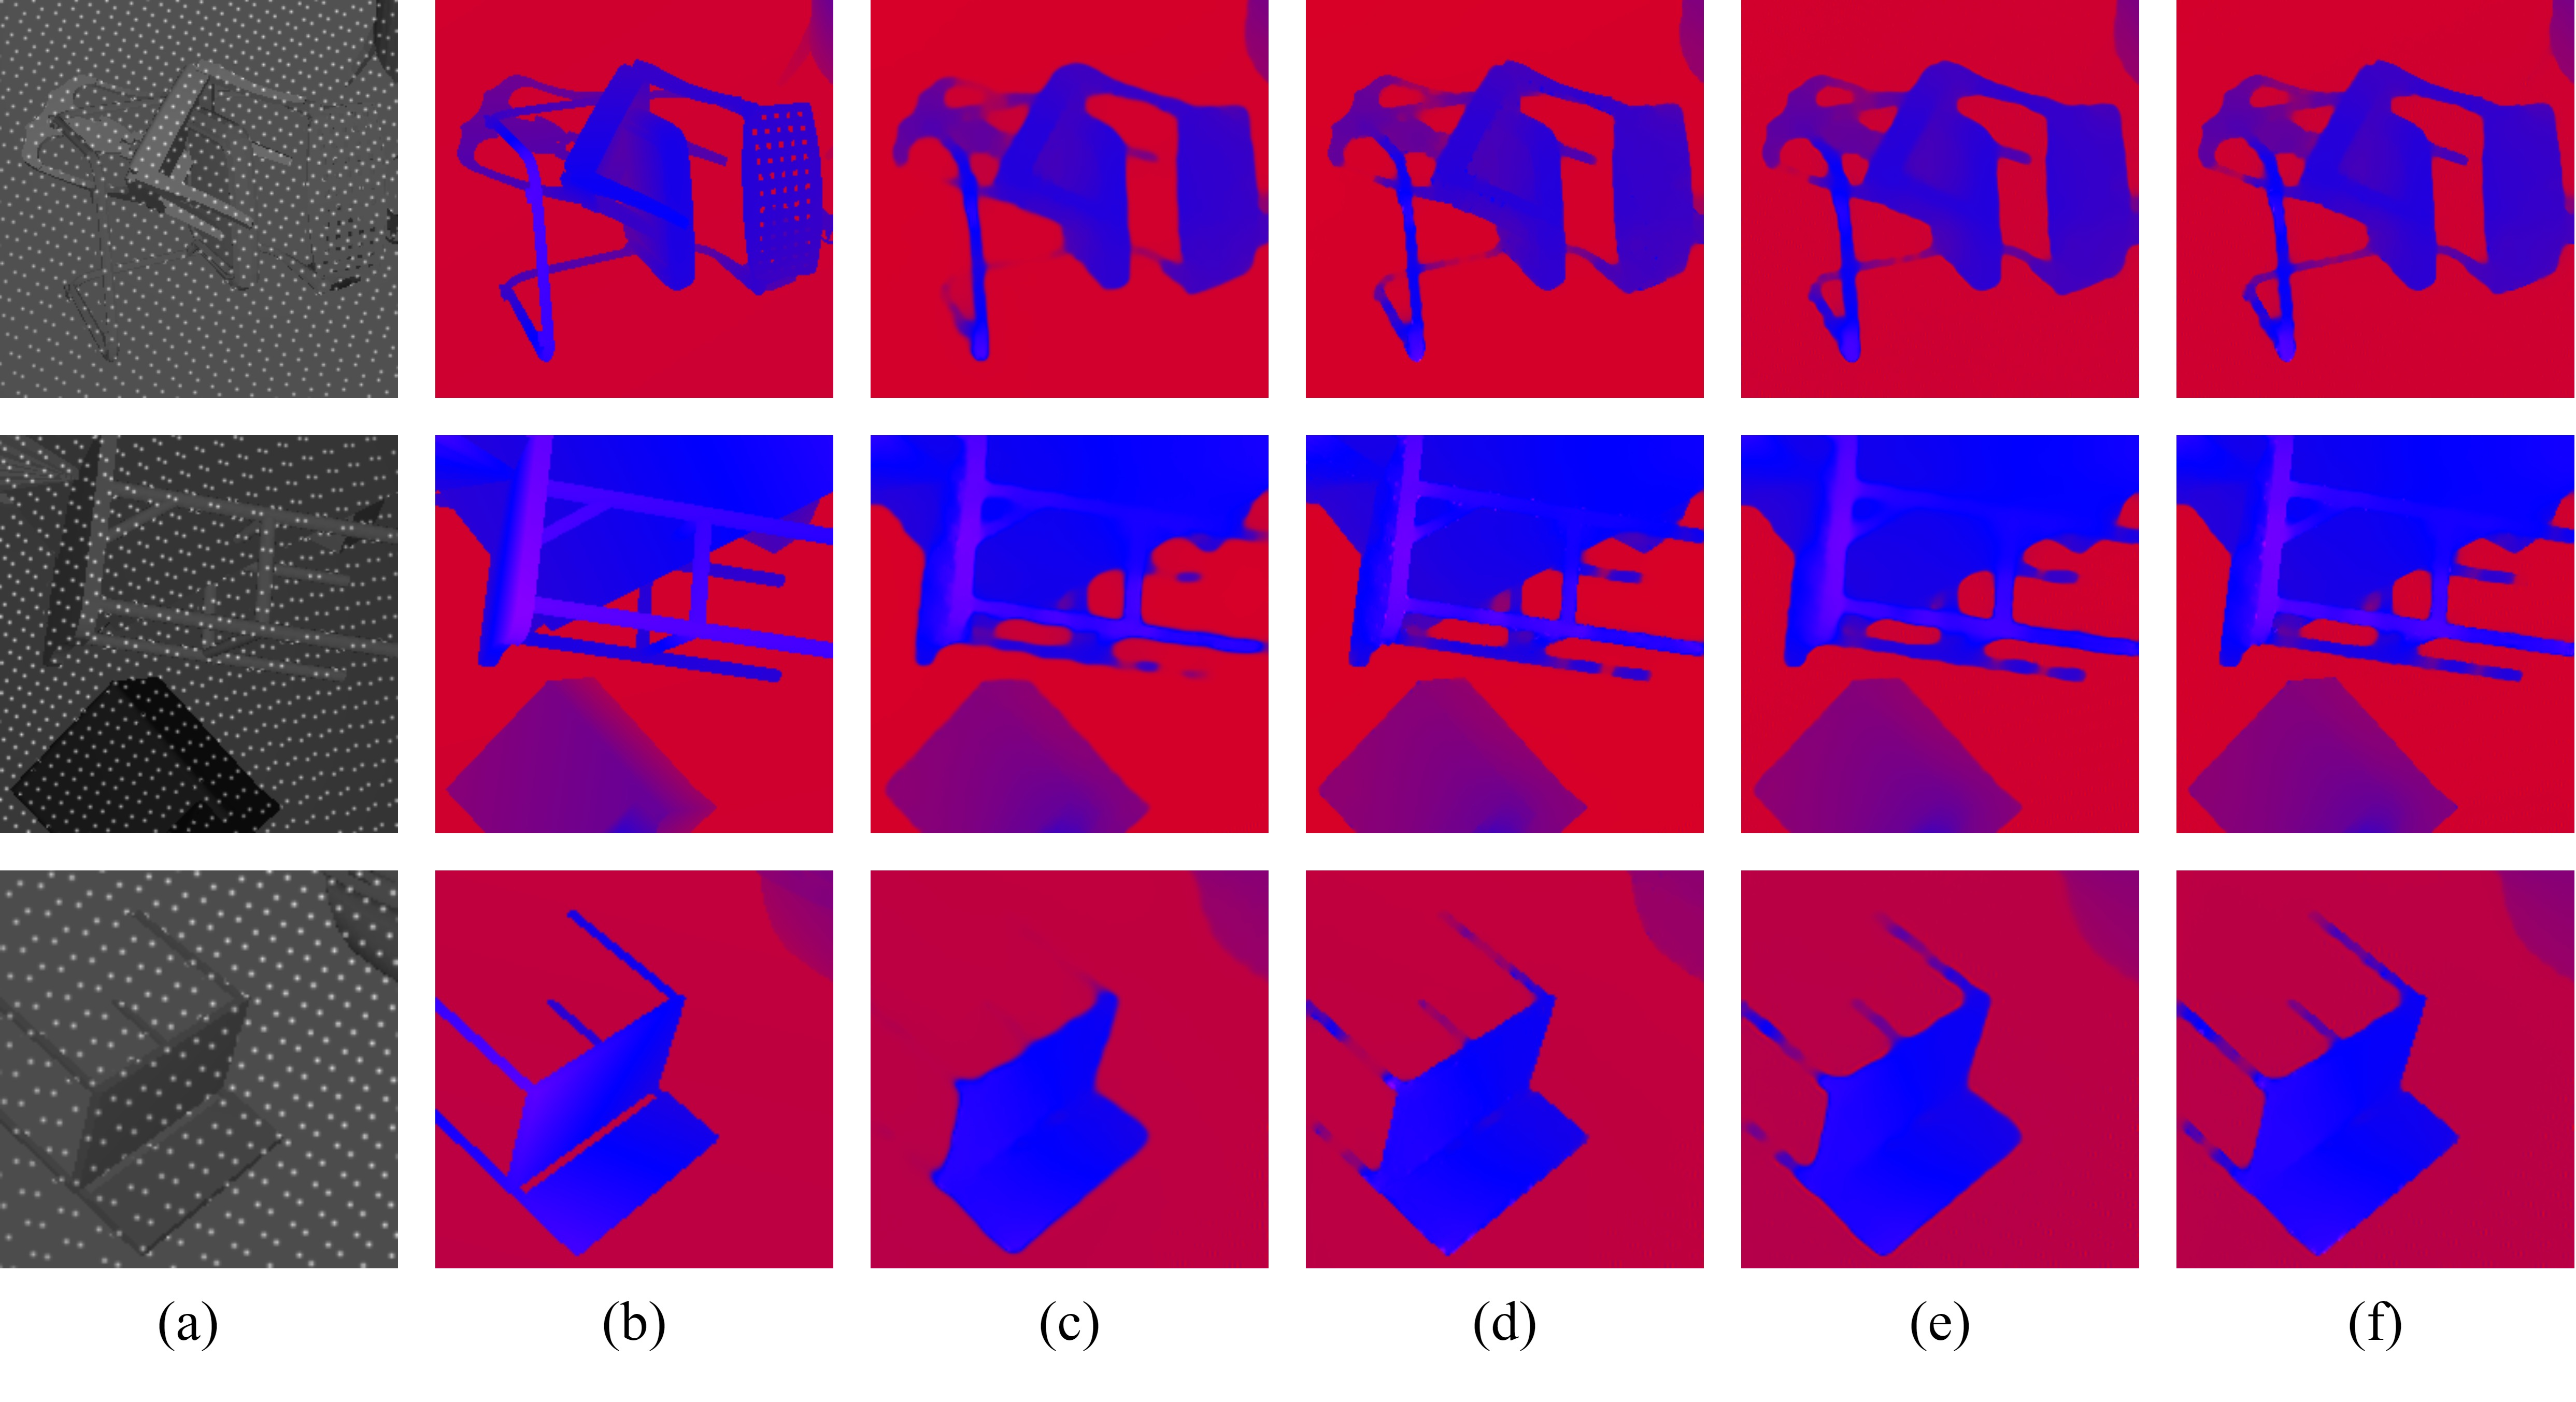
\includegraphics[width=1.0\linewidth]{images/chapter2/supp_figures/ablation_mf_masks.jpg}
    \end{center}
   \caption{Qualitative analysis of Experiment 4 in Table~\ref{table:ablation_dis_mf}, where we examine the impact of validation binary masks, introduced in Section~\ref{sec:c2_binary_masks}, on DIS-MF performance (a)~Input dot image. (b)~Ground truth disparity map. (c)~DIS-MF's output when only $\boldsymbol{M'_{FB}}$ is used to select pixels for $\boldsymbol{\mathcal{L}_{mv}}$. (d)~DIS-MF's output when $\boldsymbol{M'_{FB}}$ and $\boldsymbol{M'_{VC}}$ are used to select pixels for $\boldsymbol{\mathcal{L}_{mv}}$. (e)~DIS-MF's output when $\boldsymbol{M'_{FB}}$ and $\boldsymbol{M'_{RF}}$ are used to select pixels for $\boldsymbol{\mathcal{L}_{mv}}$. (f)~DIS-MF's output when all $\boldsymbol{M'_{FB}}$, $\boldsymbol{M'_{RF}}$, and $\boldsymbol{M'_{VC}}$ are used to select pixels for $\boldsymbol{\mathcal{L}_{mv}}$. It is noticeable how $\boldsymbol{M'_{RF}}$ contributes to completing the disparity map while $\boldsymbol{M'_{VC}}$ properly preserves the edges and discontinuities.}
    \label{fig:c2_ablation_mf_masks}
\end{figure}

\begin{figure}[t]
    \begin{center}
        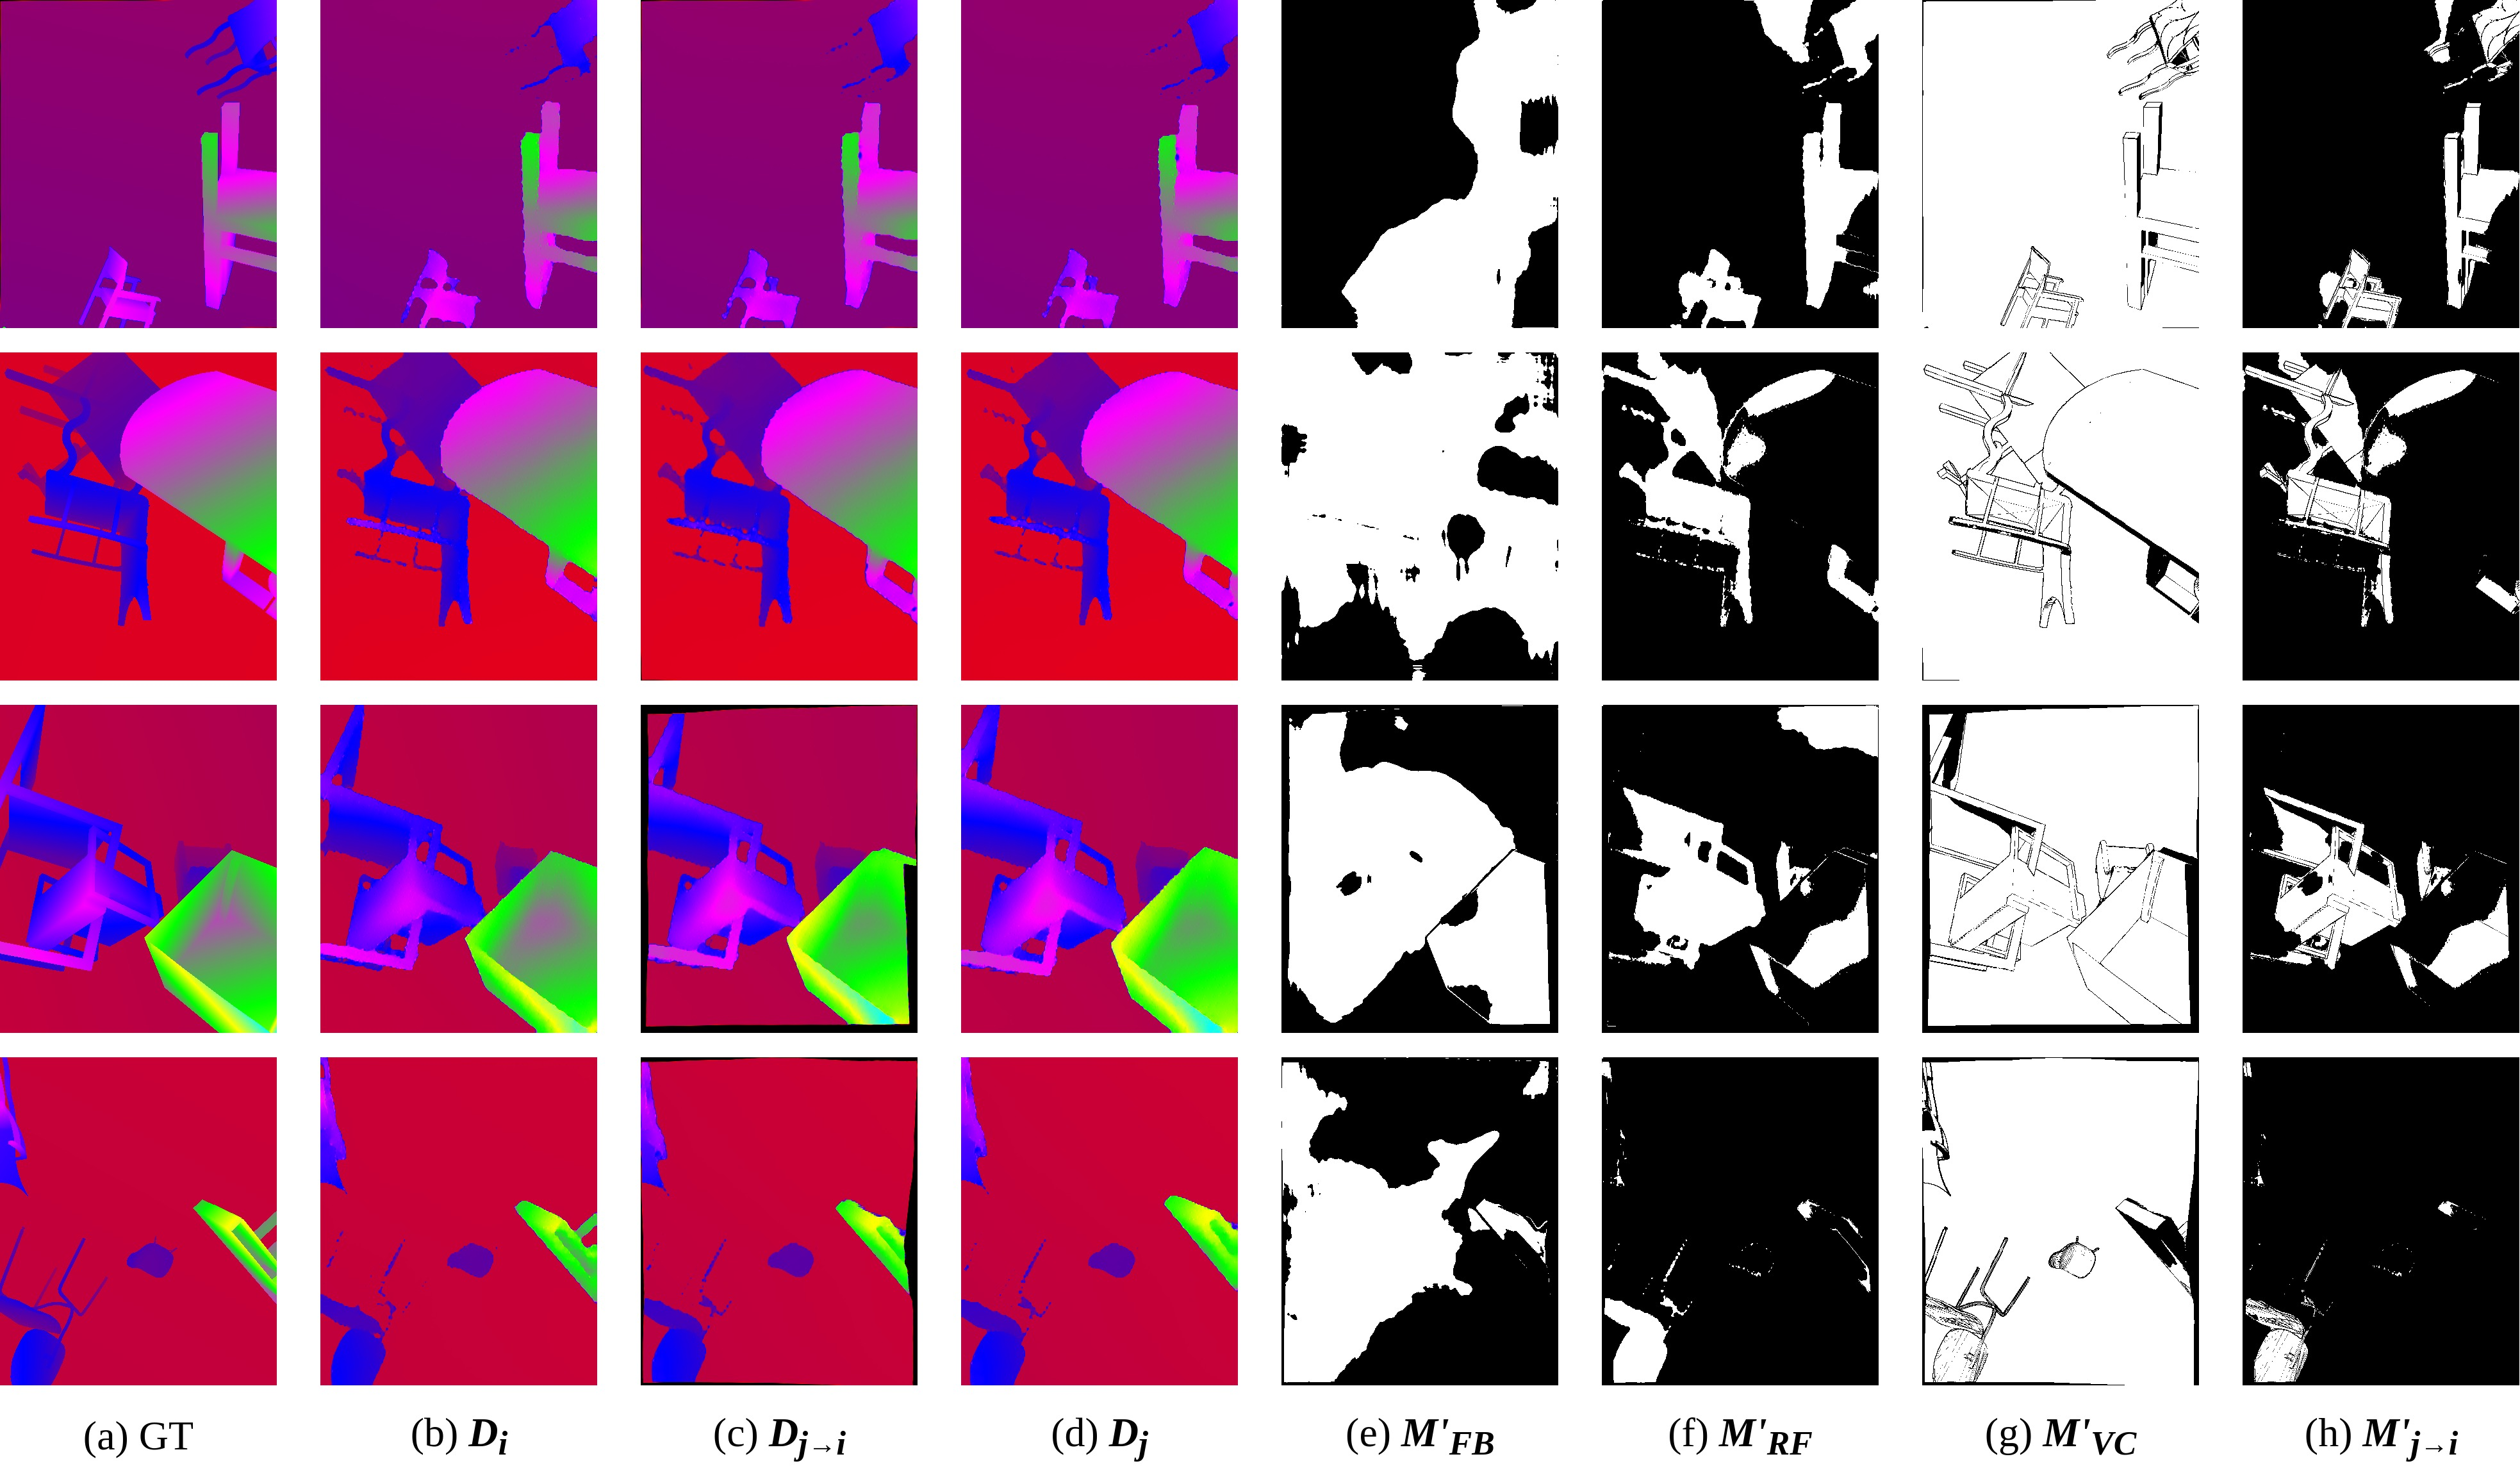
\includegraphics[width=1.0\linewidth]{images/chapter2/supp_figures/visualize_masks.jpg}
    \end{center}
   \caption{Visualizing the behavior of binary masks criteria in Section~\ref{sec:c2_binary_masks} when Frame~$j$ is being used for supervision and is warped on the Frame~$i$'s grid map. This figure demonstrates how each criterion selects high confidence pixels for training and prevents low confidence pixels from participating in the supervision and destabilizing training. (a)~Frame~$i$'s ground truth disparity map. (b)~Frame~$i$'s imperfect disparity map ($\boldsymbol{D_{i}}$). (c)~Frame~$j$'s imperfect disparity map warped on the Frame~$i$'s grid map ($\boldsymbol{D_{j \rightarrow i}}$). (d)~Frame~$j$'s imperfect disparity map ($\boldsymbol{D_{j}}$). (e)~Optical flow forward-backward consistency mask~$\boldsymbol{M'_{FB}}$. (f)~Optical flow and rigid flow consistency mask~$\boldsymbol{M'_{RF}}$. (g)~Visual consistency of ambient images mask~$\boldsymbol{M'_{VC}}$. (h)~The intersection of all binary masks~$\boldsymbol{M'_{j \rightarrow i}} = \boldsymbol{M'_{FB}} \odot \boldsymbol{M'_{RF}} \odot \boldsymbol{M'_{VC}}$.}
    \label{fig:c2_visualize_masks}
\end{figure}

\subsubsection{Utilizing the Fusion Architecture in Different Setups}
This section analyzes the effect of three factors in our DIS-MF model's performance: the imperfect input disparities, the fusion architecture, and our proposed multi-view-based loss function. In this regard, we applied our DIS-MF network to CTD outputs and trained the fusion model once with CTD loss function and once with ours. Comparison of the results with the original CTD and DIS models in Table~\ref{table:ablation_ctd_dis_mf} discriminates the individual efficacy of our proposed loss and fusion architecture and shows these two contributions are complementary to each other. Also, the table suggests that these two are not necessarily required to be applied to DIS-SF imperfect disparities, as they can significantly improve the quality of CTD outputs.

\subsubsection{Robustness to Optical Flow Predictions} \label{sec:c2_ablation_gma}
As discussed in Section~\ref{sec:c2_liteflownet}, our training process is robust to optical flow prediction errors thanks to our validation masks introduced in Section~\ref{sec:c2_binary_masks}. This robustness allows us to utilize the lightweight optical flow network LiteFlowNet~\cite{hui2018liteflownet} in our models. To evaluate this robustness, we also trained our networks on the synthetic data with the state-of-the-art optical flow model on MPI Sintel~\cite{butler2012naturalistic}, GMA~\cite{jiang2021learning}, which has \textbf{69.4}\% higher accuracy but is slower than LiteFlowNet. The results in Table~\ref{table:ablation_gma} show that despite the huge gap between the GMA and LiteFlowNet accuracies, the gain that GMA brings to our models is marginal. It is also notable that since our validation masks in DIS-MF are stricter than in DIS-SF on account of having access to imperfect disparities (see Section~\ref{sec:c2_binary_masks}), DIS-MF is more robust to the optical flow performance.


\begin{table}[t]
    \begin{center}
        \begin{tabular}{lcccc}
        \hline
        Model & $o(0.5)$ & $o(1)$ & $o(2)$ & $o(5)$ \\
        \hline
        CTD & 3.38 & 1.71 & 0.85 & 0.28 \\
        DIS-SF & 2.31 & 1.24 & 0.62 & 0.19 \\
        \arrayrulecolor{lightgray}\hline\arrayrulecolor{black}
        CTD Out. + DIS-MF Net. + CTD Loss & 2.33 & 1.14 & 0.60 & 0.20 \\
        CTD Out. + DIS-MF Net. + DIS Loss & 1.97 & 0.83 & 0.37 & 0.12 \\
        DIS-MF & \textbf{1.58} & \textbf{0.71} & \textbf{0.32} & \textbf{0.10} \\
        \hline
        \end{tabular}
    \end{center}
    \caption{Analysis of our multi-frame fusion efficacy when it takes CTD outputs as imperfect input disparities.}
    \label{table:ablation_ctd_dis_mf}
\end{table}


\begin{table}[t]
    \begin{center}
        \begin{tabular}{lcccc}
        \hline
        Model & $o(0.5)$ & $o(1)$ & $o(2)$ & $o(5)$ \\
        \hline
        DIS-SF + LiteFlowNet & 2.31 & 1.24 & 0.62 & 0.19 \\
        DIS-SF + GMA & \textbf{2.14} & \textbf{1.12} & \textbf{0.56} & \textbf{0.14} \\
        \hline
        DIS-MF + LiteFlowNet & \textbf{1.58} & \textbf{0.71} & 0.32 & 0.10 \\
        DIS-MF + GMA & 1.62 & \textbf{0.71} & \textbf{0.31} & \textbf{0.09} \\
        \hline
        \end{tabular}
    \end{center}
    \caption{Analysis of the effect of using different optical flow networks (LiteFlowNet~\cite{hui2018liteflownet} and GMA~\cite{jiang2021learning}) on DIS models' performances.}
    \label{table:ablation_gma}
\end{table}

\subsection{Additional Qualitative Results} \label{sec:c2_additional_results}
Here we first present an extended qualitative analysis of existing models along with our proposed models in Figures~\ref{fig:c2_kinect_results}, \ref{fig:c2_sim_results}, \ref{fig:c2_actual_results}, and \ref{fig:c2_real_results}. Each figure presents sample images from one of the datasets introduced in the main paper. The color bars provided for disparity error maps (in terms of pixels) in the figures are also valid for the images in the main article.

Furthermore, we adopt a different approach to visualize depth maps of objects from the synthetic dataset in Figure~\ref{fig:c2_rendered} and from the real dataset in Figure~\ref{fig:c2_rendered_real}. To visualize the depth maps, we rely on color-coded depth values and 3D rendering of the scene. The depths are rendered in OpenGL~\cite{shreiner2013opengl}, where every point of the mesh has a color that corresponds to its depth value in the Turbo colormap~\cite{mikhailov2019turbo}. In addition, we place a spotlight at the same position as the camera to light the scene. This allows us to better appreciate the quality of the computed depths as small changes of the values of the normals in the mesh impact the lighting. Finally, we consider that edges over 10 cm in the mesh are invalid and exclude them from the rendered images.


\begin{figure}
    \begin{center}
        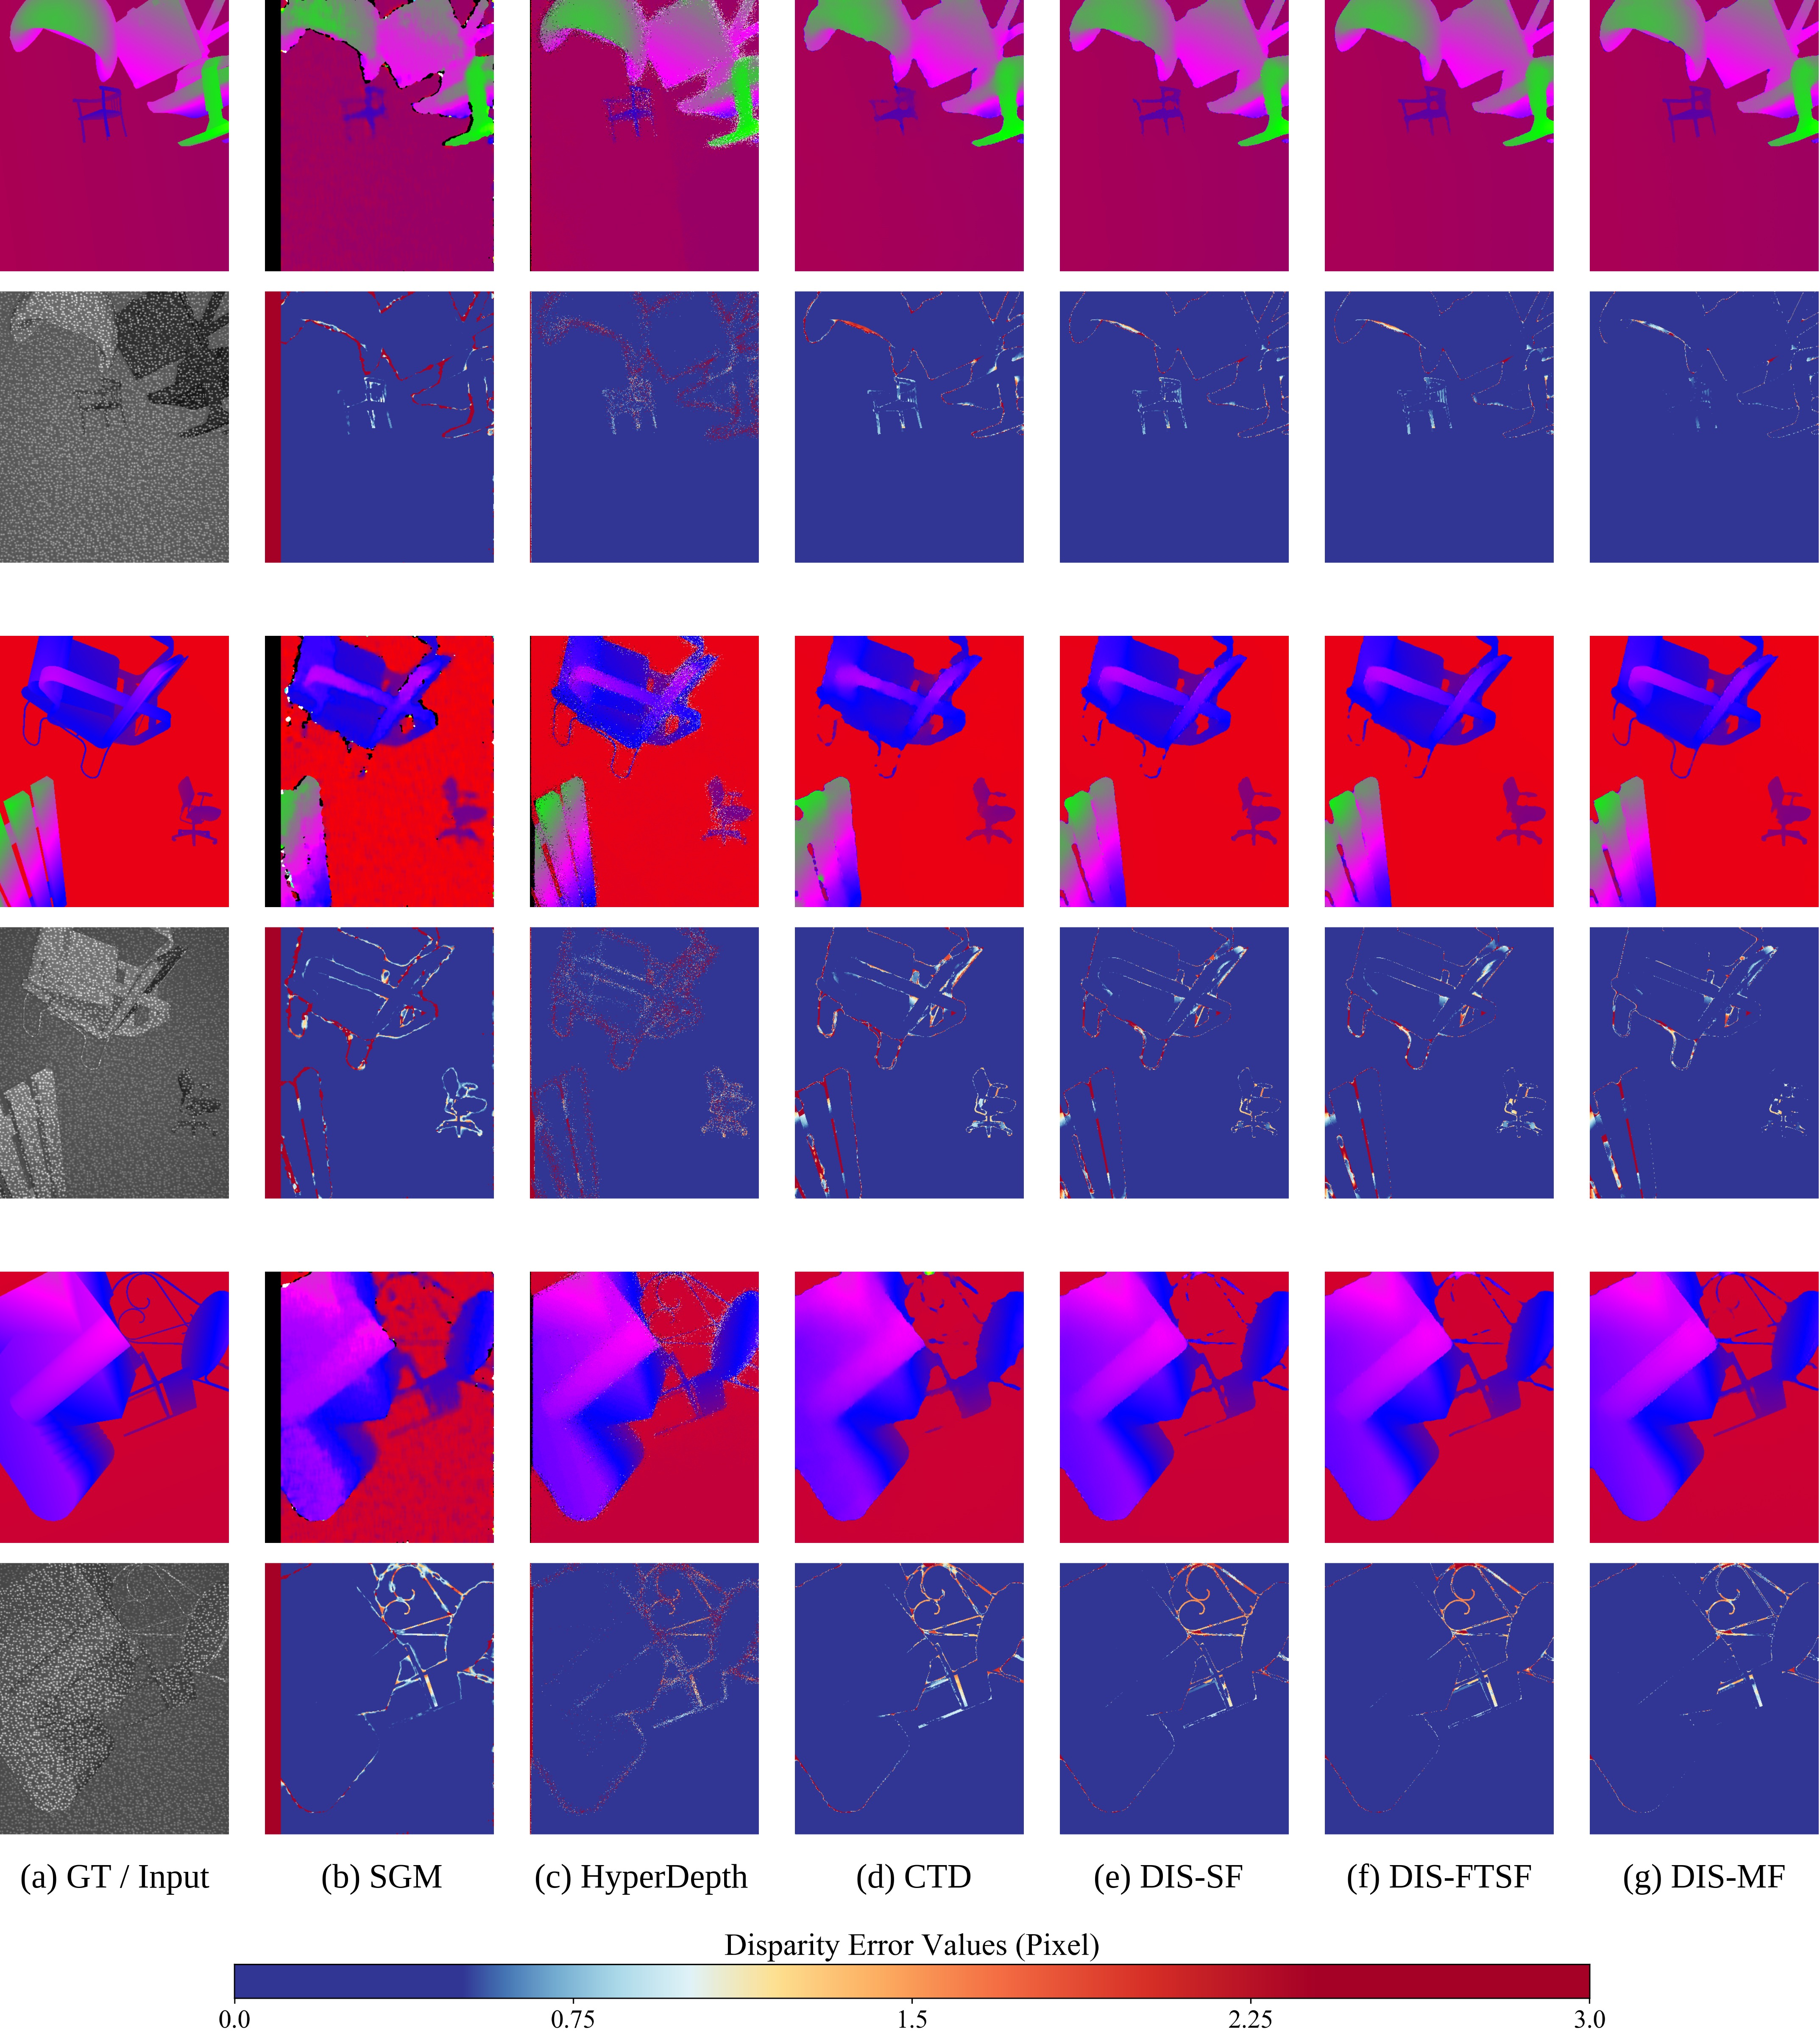
\includegraphics[width=1\linewidth]{images/chapter2/supp_figures/supp_results_1.jpg}
    \end{center}
   \caption{Additional full-size qualitative results of the implemented methods and their corresponding error maps. All samples are taken from the synthetic dataset rendered with Kinect dot pattern. (a)~Ground truth disparity map and input dot image. (b)~The SGM algorithm~\cite{hirschmuller2007stereo}. (c)~HyperDepth~\cite{ryan2016hyperdepth}. (d)~CTD~\cite{riegler2019connecting}. (e)~Our DepthInSpace Single-Frame (DIS-SF) model. (f)~Our DepthInSpace Fine-Tuned Single-Frame (DIS-FTSF) model. (g)~Our DepthInSpace Multi-Frame (DIS-MF) Model.}
    \label{fig:c2_kinect_results}
\end{figure}

\begin{figure}
    \begin{center}
        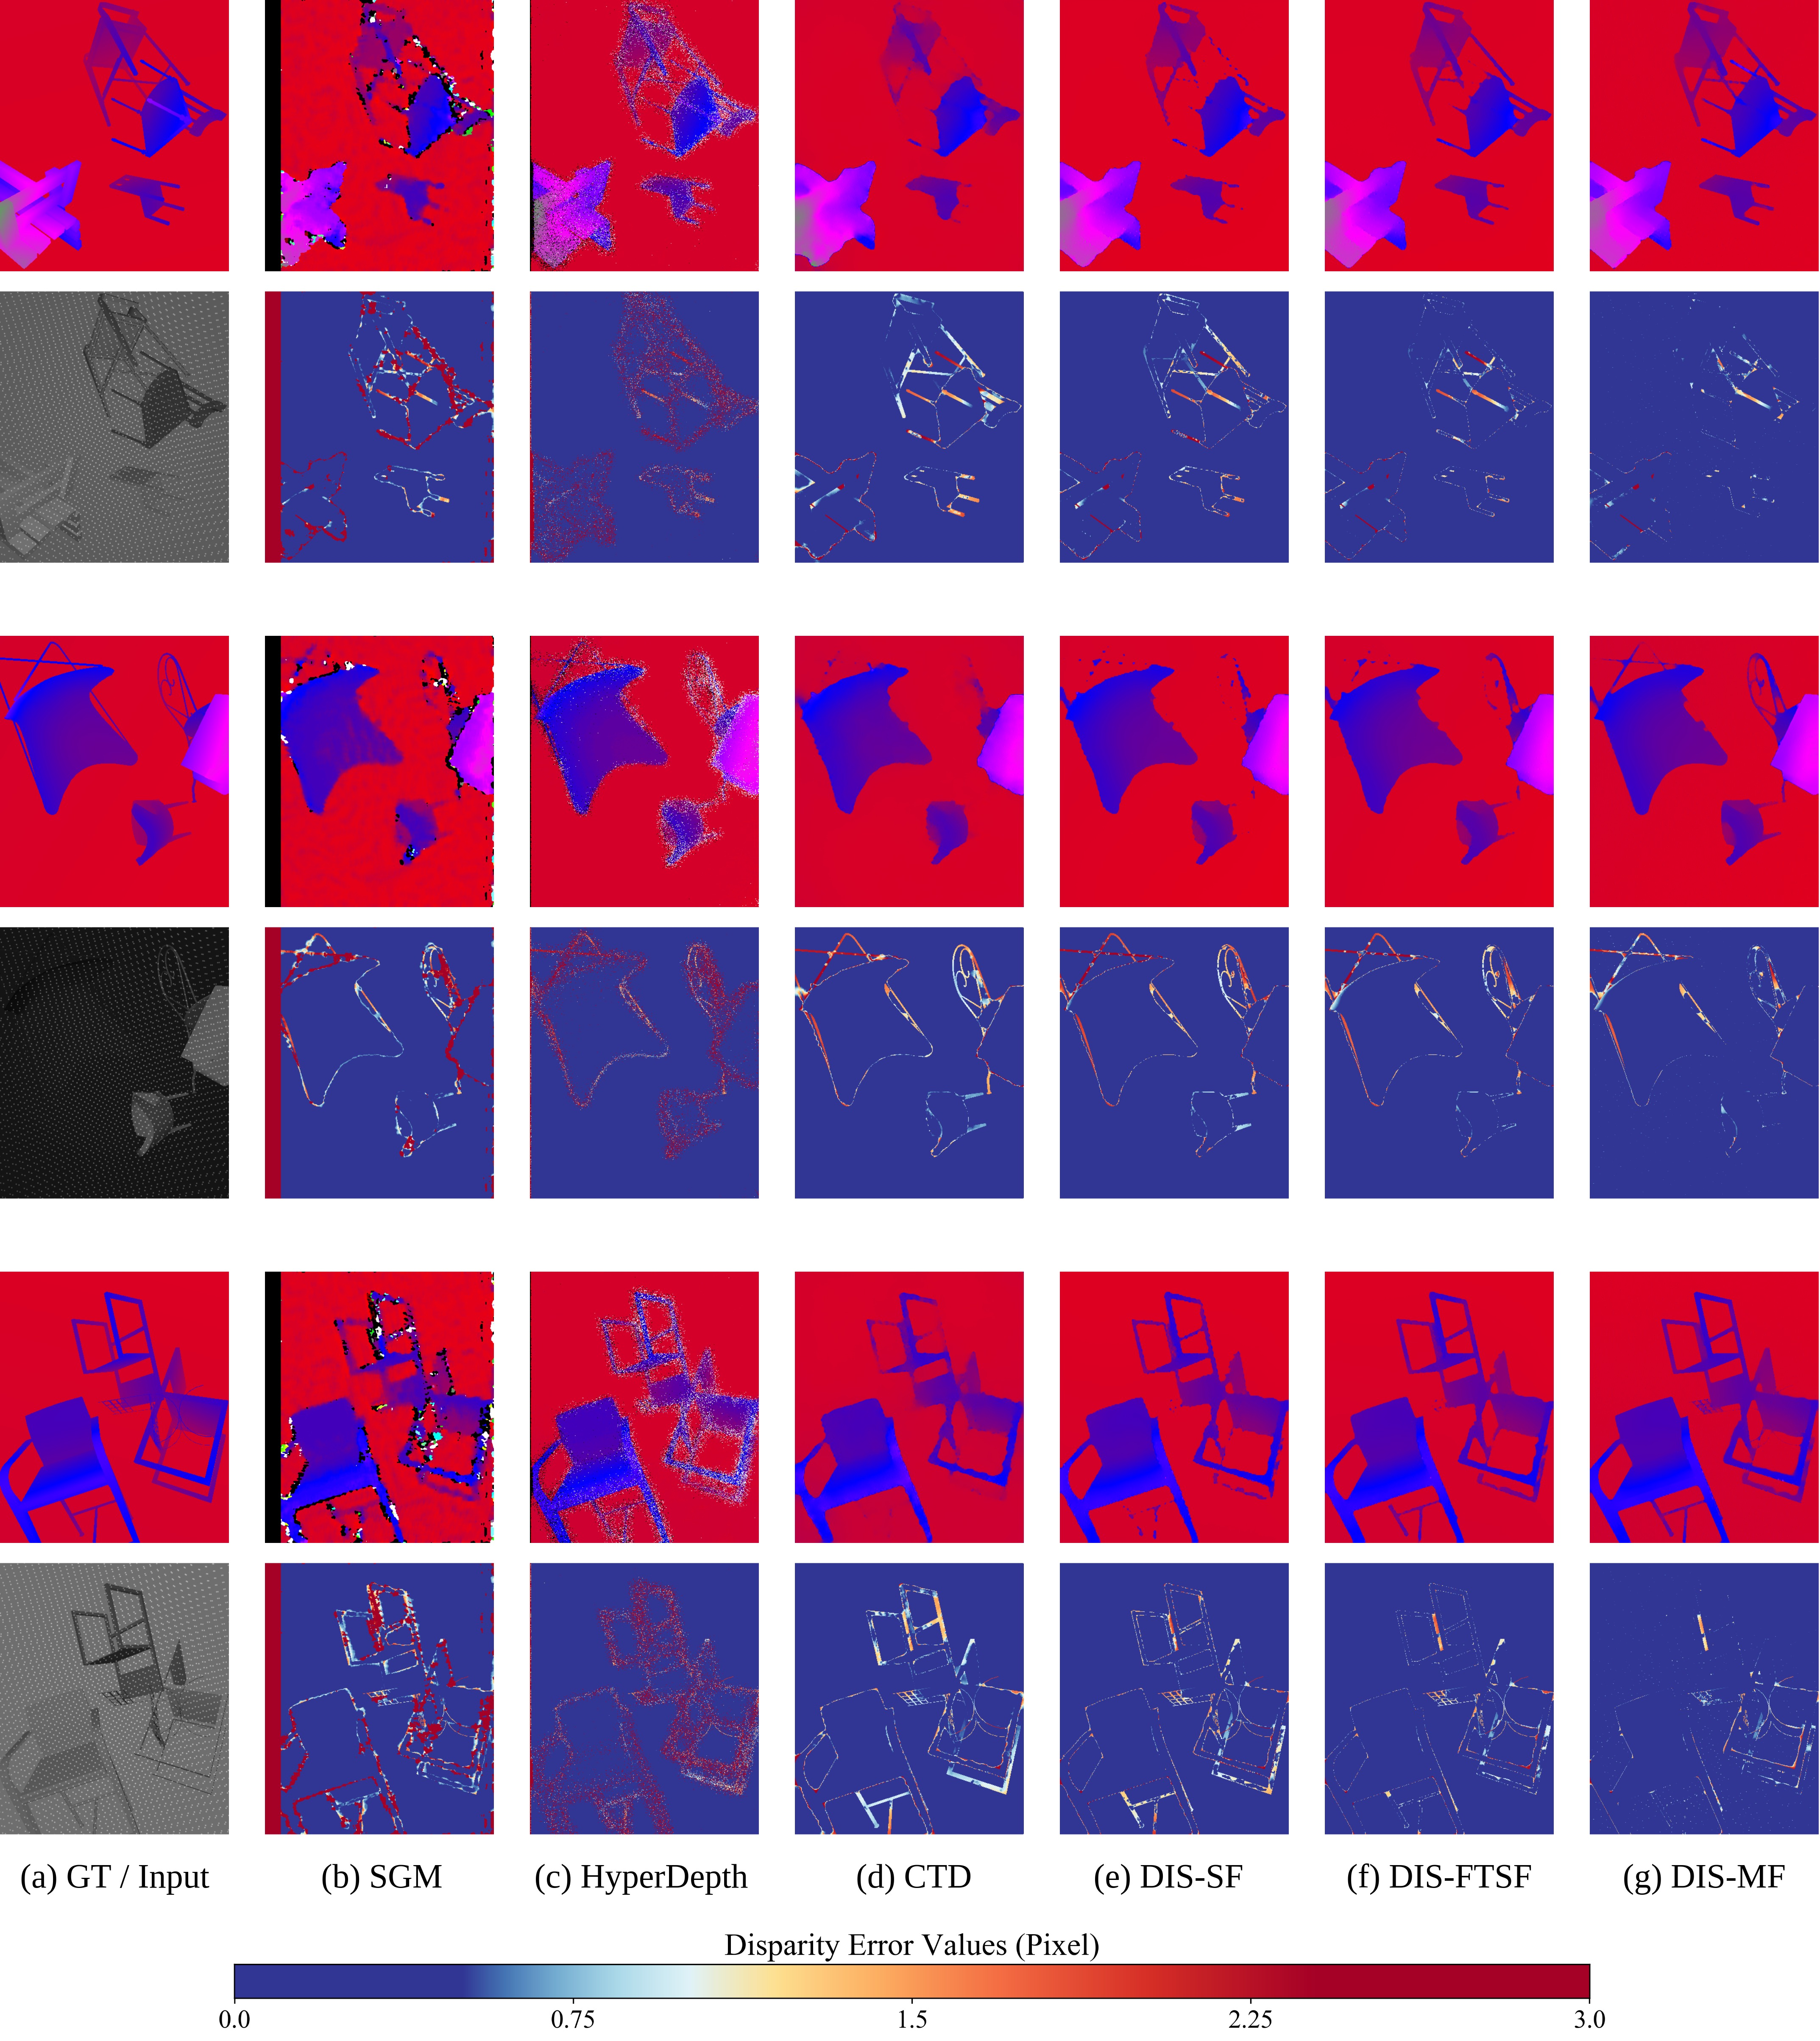
\includegraphics[width=1\linewidth]{images/chapter2/supp_figures/supp_results_2.jpg}
    \end{center}
   \caption{Additional full-size qualitative results of the implemented methods and their corresponding error maps. All samples are taken from the synthetic dataset rendered with our own theoretical dot pattern. (a)~Ground truth disparity map and input dot image with projected pattern. (b)~The SGM algorithm~\cite{hirschmuller2007stereo}. (c)~HyperDepth~\cite{ryan2016hyperdepth}. (d)~CTD~\cite{riegler2019connecting}. (e)~Our DepthInSpace Single-Frame (DIS-SF) model. (f)~Our DepthInSpace Fine-Tuned Single-Frame (DIS-FTSF) model. (g)~Our DepthInSpace Multi-Frame (DIS-MF) Model.}
    \label{fig:c2_sim_results}
\end{figure}

\begin{figure}
    \begin{center}
        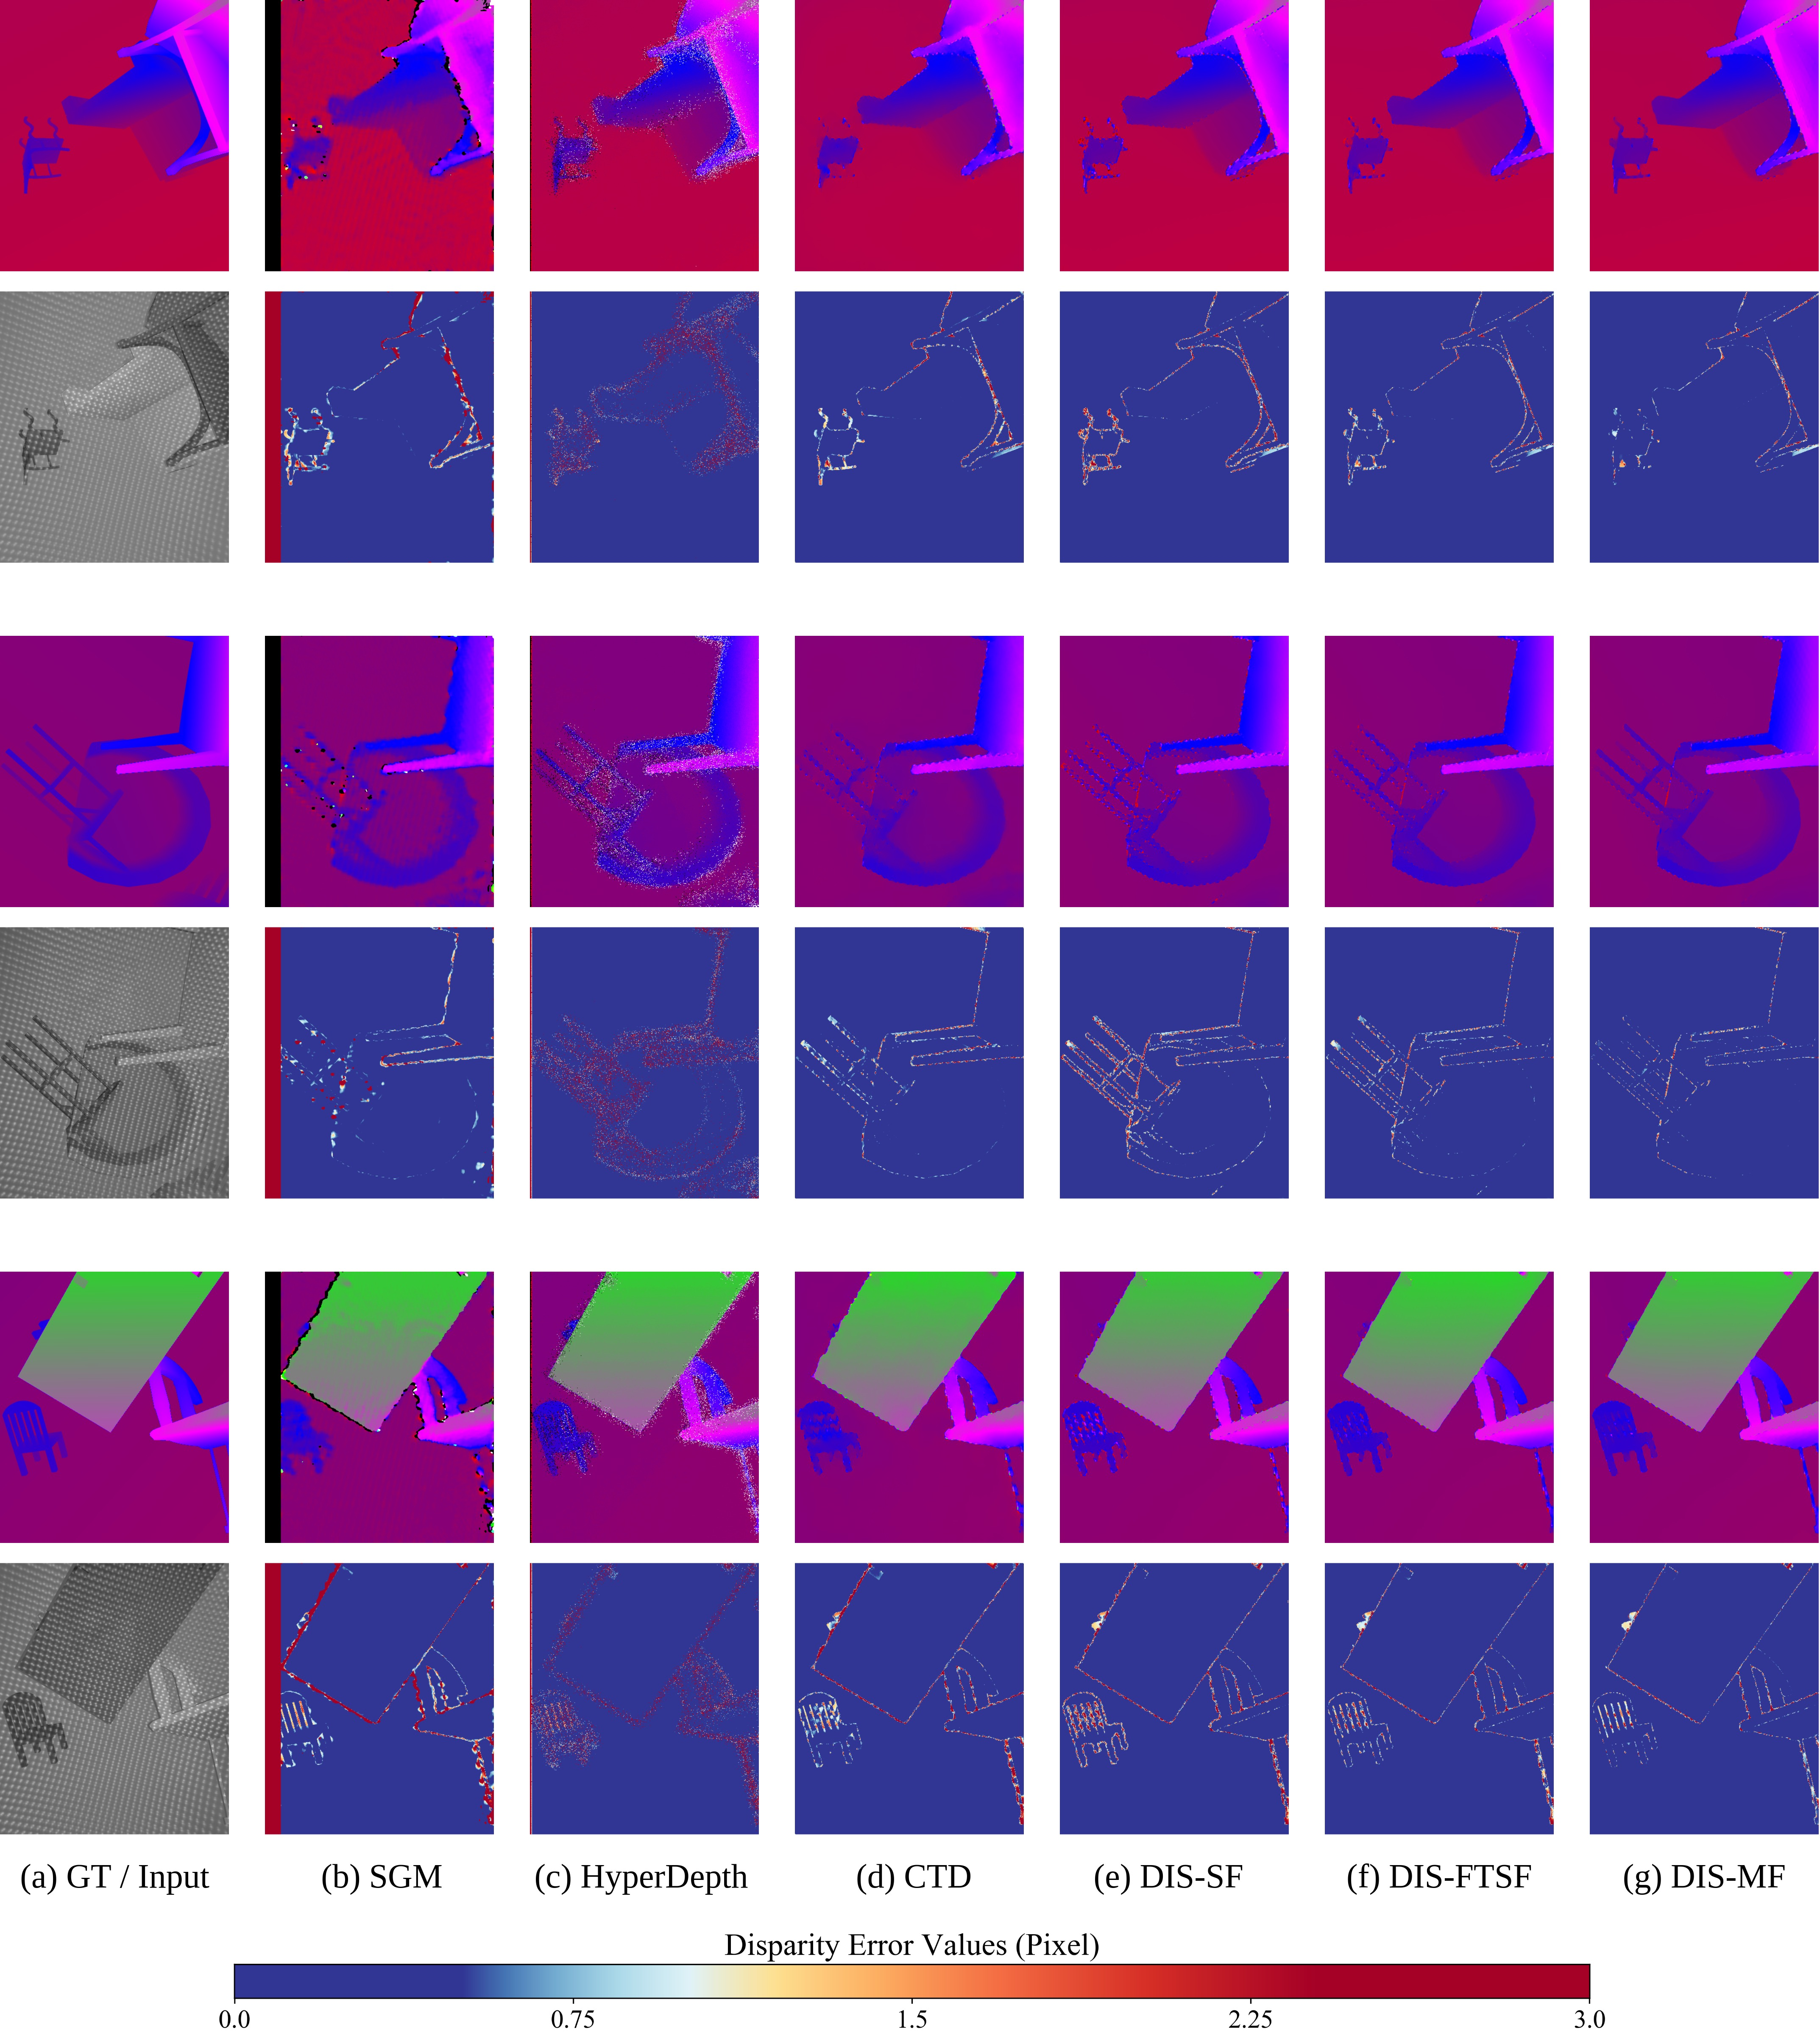
\includegraphics[width=1\linewidth]{images/chapter2/supp_figures/supp_results_3.jpg}
    \end{center}
   \caption{Additional full-size qualitative results of the implemented methods and their corresponding error maps. All samples are taken from the synthetic dataset rendered with our own dot pattern observed in an actual laboratory setup. (a)~Ground truth disparity map and input dot image. (b)~The SGM algorithm~\cite{hirschmuller2007stereo}. (c)~HyperDepth~\cite{ryan2016hyperdepth}. (d)~CTD~\cite{riegler2019connecting}. (e)~Our DepthInSpace Single-Frame (DIS-SF) model. (f)~Our DepthInSpace Fine-Tuned Single-Frame (DIS-FTSF) model. (g)~Our DepthInSpace Multi-Frame (DIS-MF) Model.}
    \label{fig:c2_actual_results}
\end{figure}

\begin{figure}
    \begin{center}
        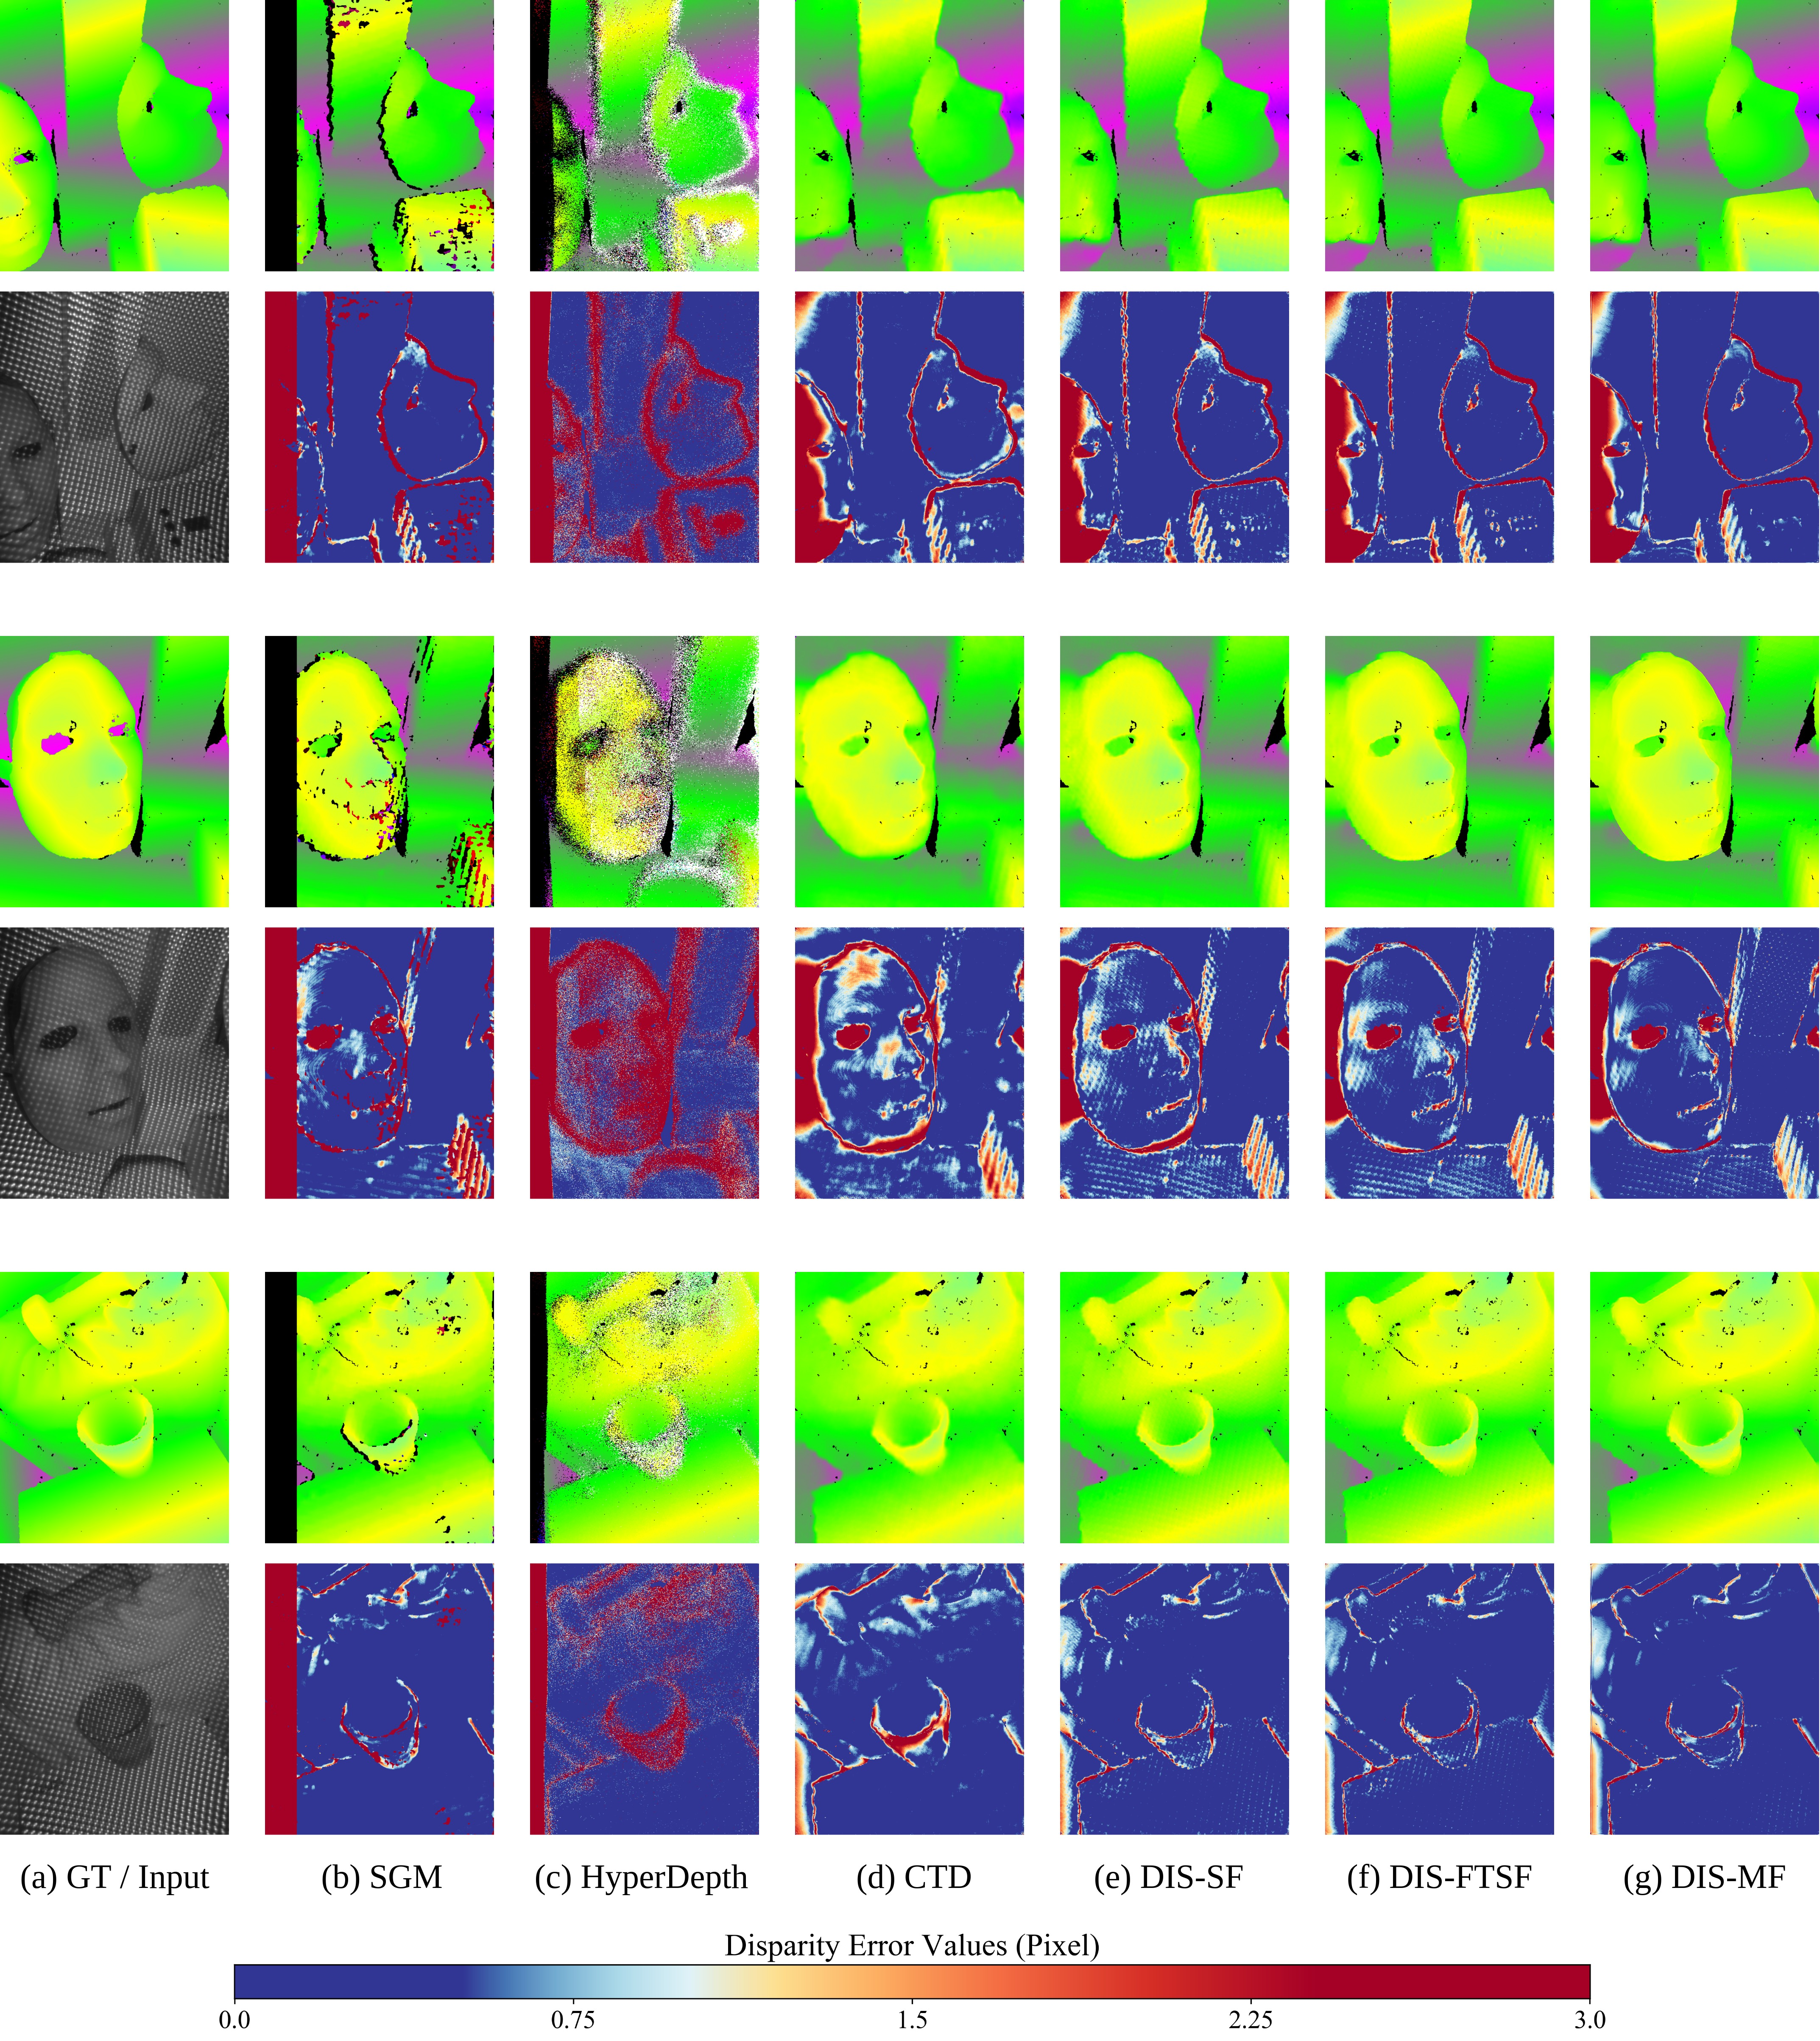
\includegraphics[width=1\linewidth]{images/chapter2/supp_figures/supp_results_4.jpg}
    \end{center}
   \caption{Additional full-size qualitative results of the implemented methods and their corresponding error maps. All samples are taken from the real dataset. (a)~Ground truth disparity map and input dot image. (b)~The SGM algorithm~\cite{hirschmuller2007stereo}. (c)~HyperDepth~\cite{ryan2016hyperdepth}. (d)~CTD~\cite{riegler2019connecting}. (e)~Our DepthInSpace Single-Frame (DIS-SF) model. (f)~Our DepthInSpace Fine-Tuned Single-Frame (DIS-FTSF) model. (g)~Our DepthInSpace Multi-Frame (DIS-MF) Model. Points for which the ground truth data is unavailable are excluded from evaluation.}
    \label{fig:c2_real_results}
\end{figure}

\begin{figure}[t]
    \begin{center}
        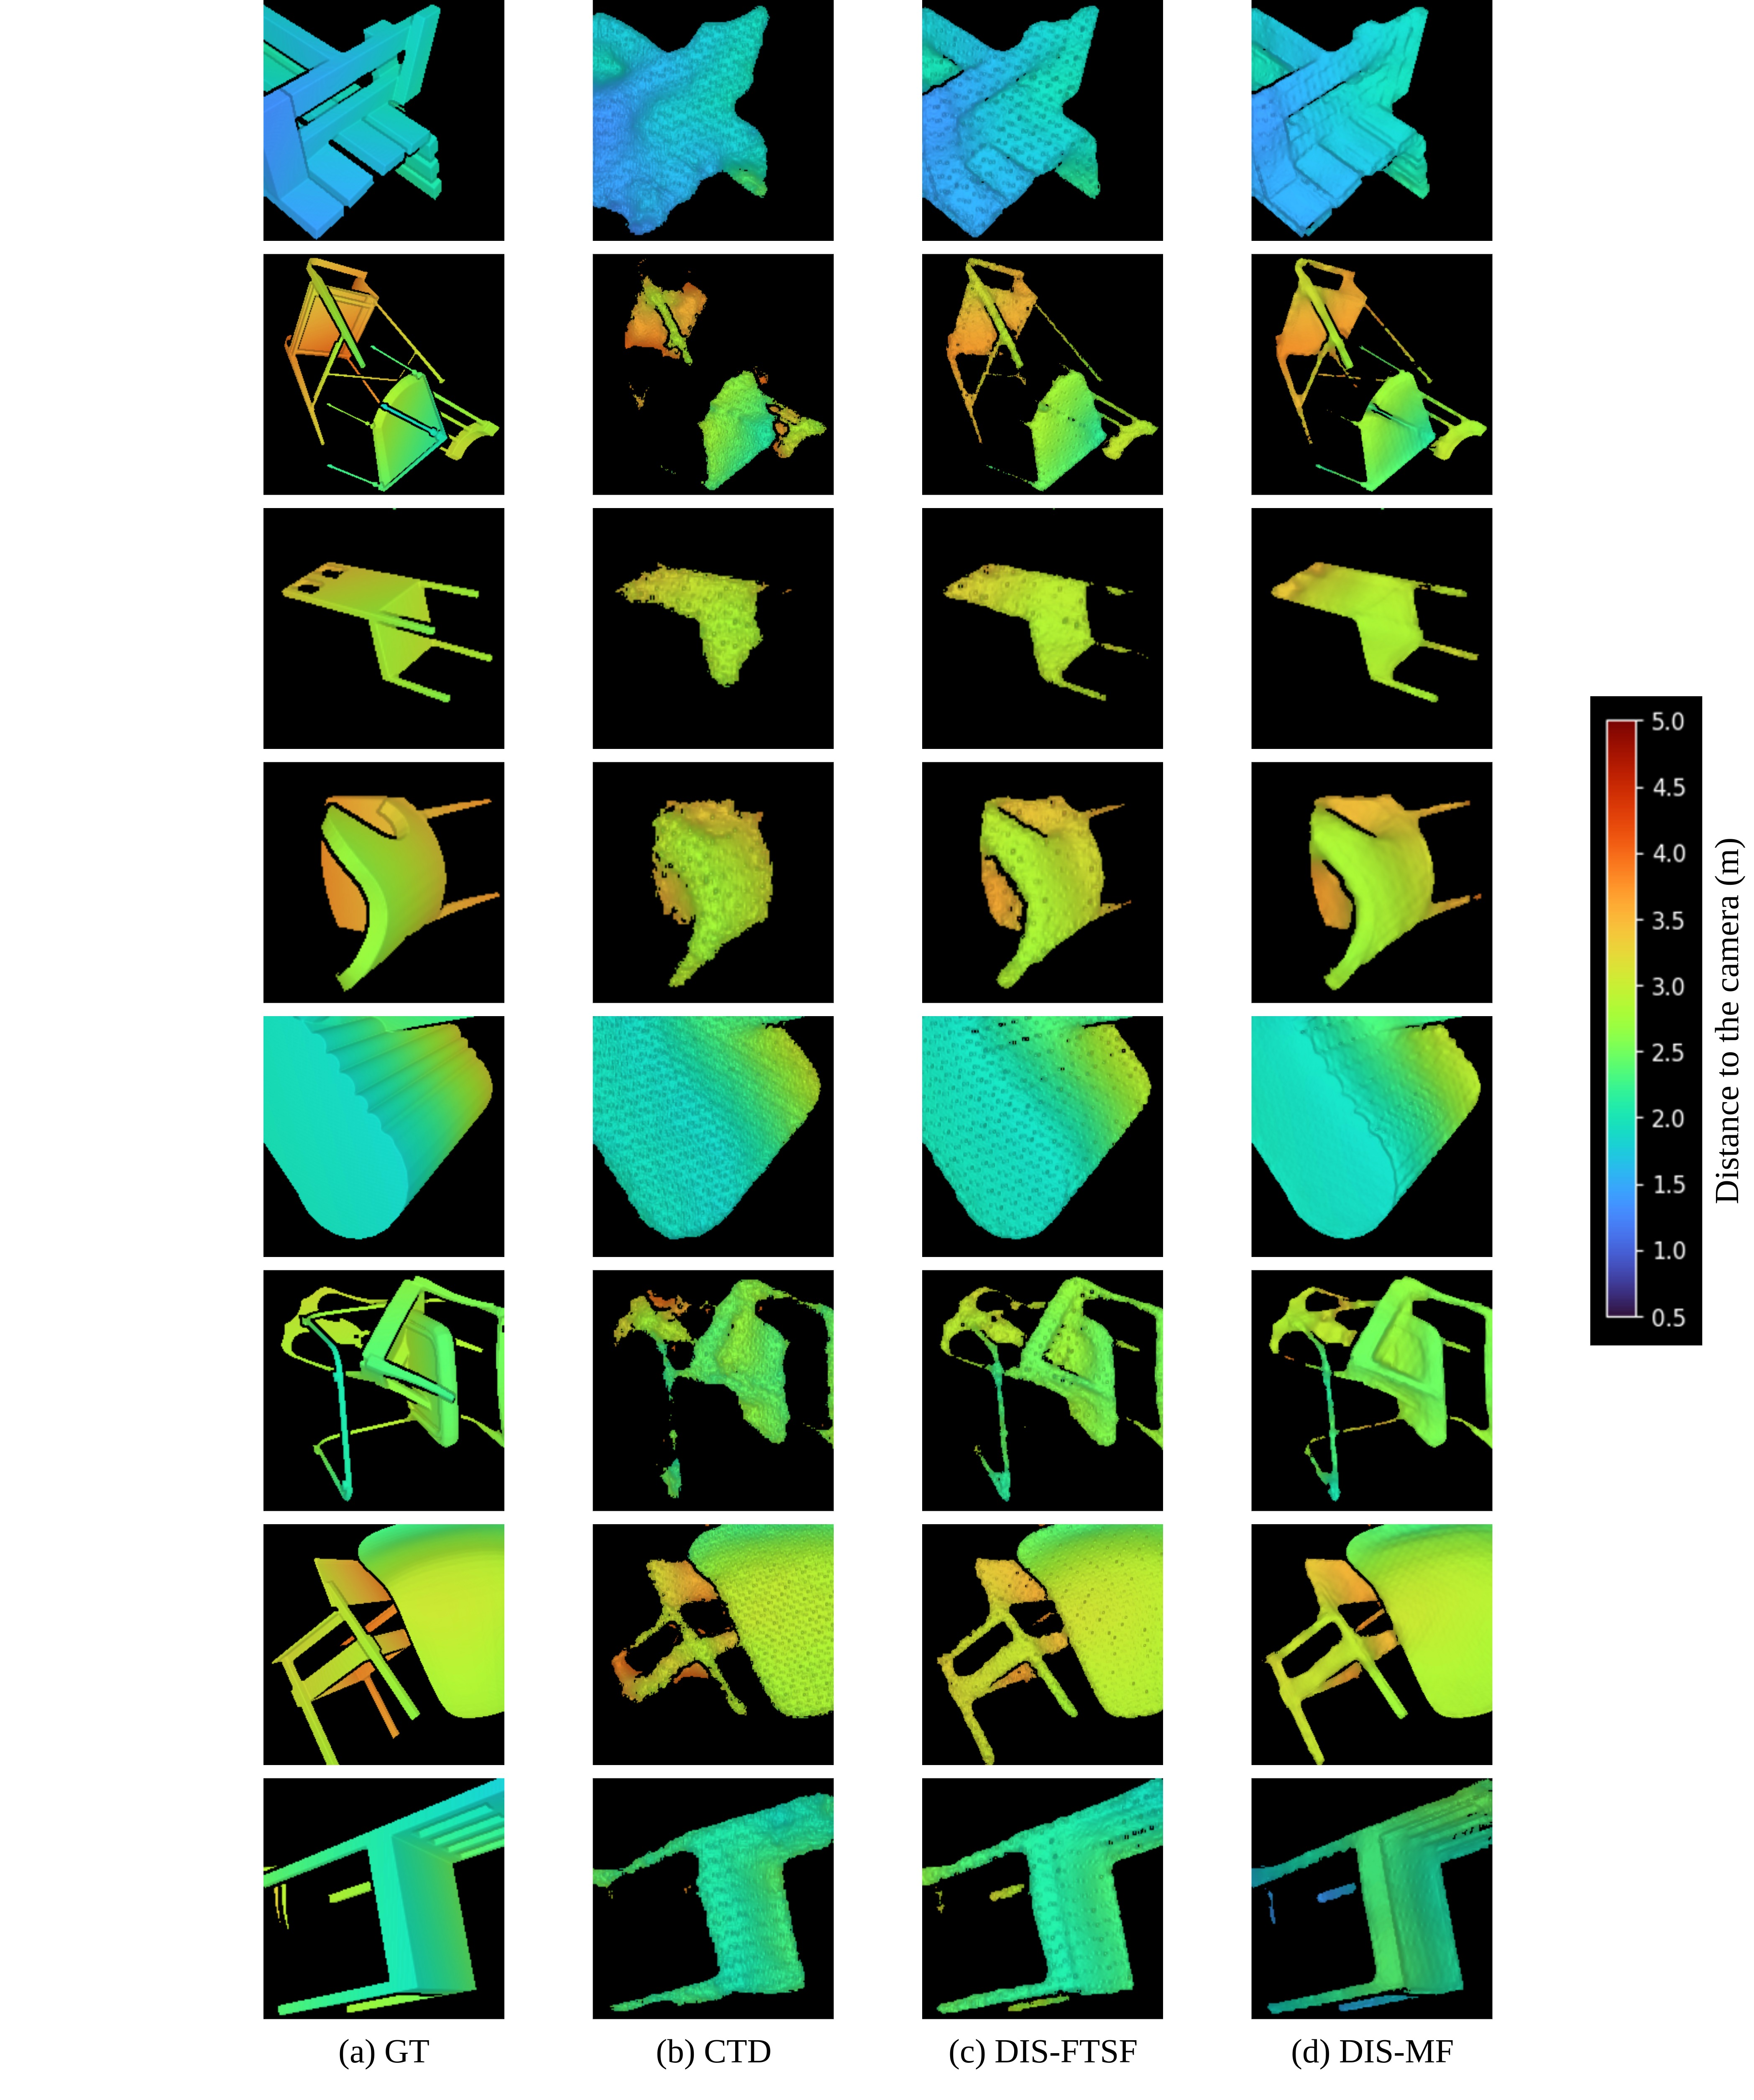
\includegraphics[width=1.0\linewidth]{images/chapter2/supp_figures/rendered.jpg}
    \end{center}
   \caption{Qualitative analysis of the depth maps rendered in OpenGL~\cite{shreiner2013opengl} and presented in the Turbo color map~\cite{mikhailov2019turbo}. Samples are taken from the synthetic dataset. This analysis shows how our models outperform the state-of-the-art model, CTD~\cite{riegler2019connecting}, in preserving details of the 3D objects and producing sharp edges. (a)~Ground truth depth map. (b)~CTD~\cite{riegler2019connecting}. (c)~Our DIS-FTSF model. (d)~Our DIS-MF model. For further information about 3D rendering of depth maps, refer to Section~\ref{sec:c2_additional_results}. The color bar represents depth values in meters.}
    \label{fig:c2_rendered}
\end{figure}

\begin{figure}[t]
    \begin{center}
    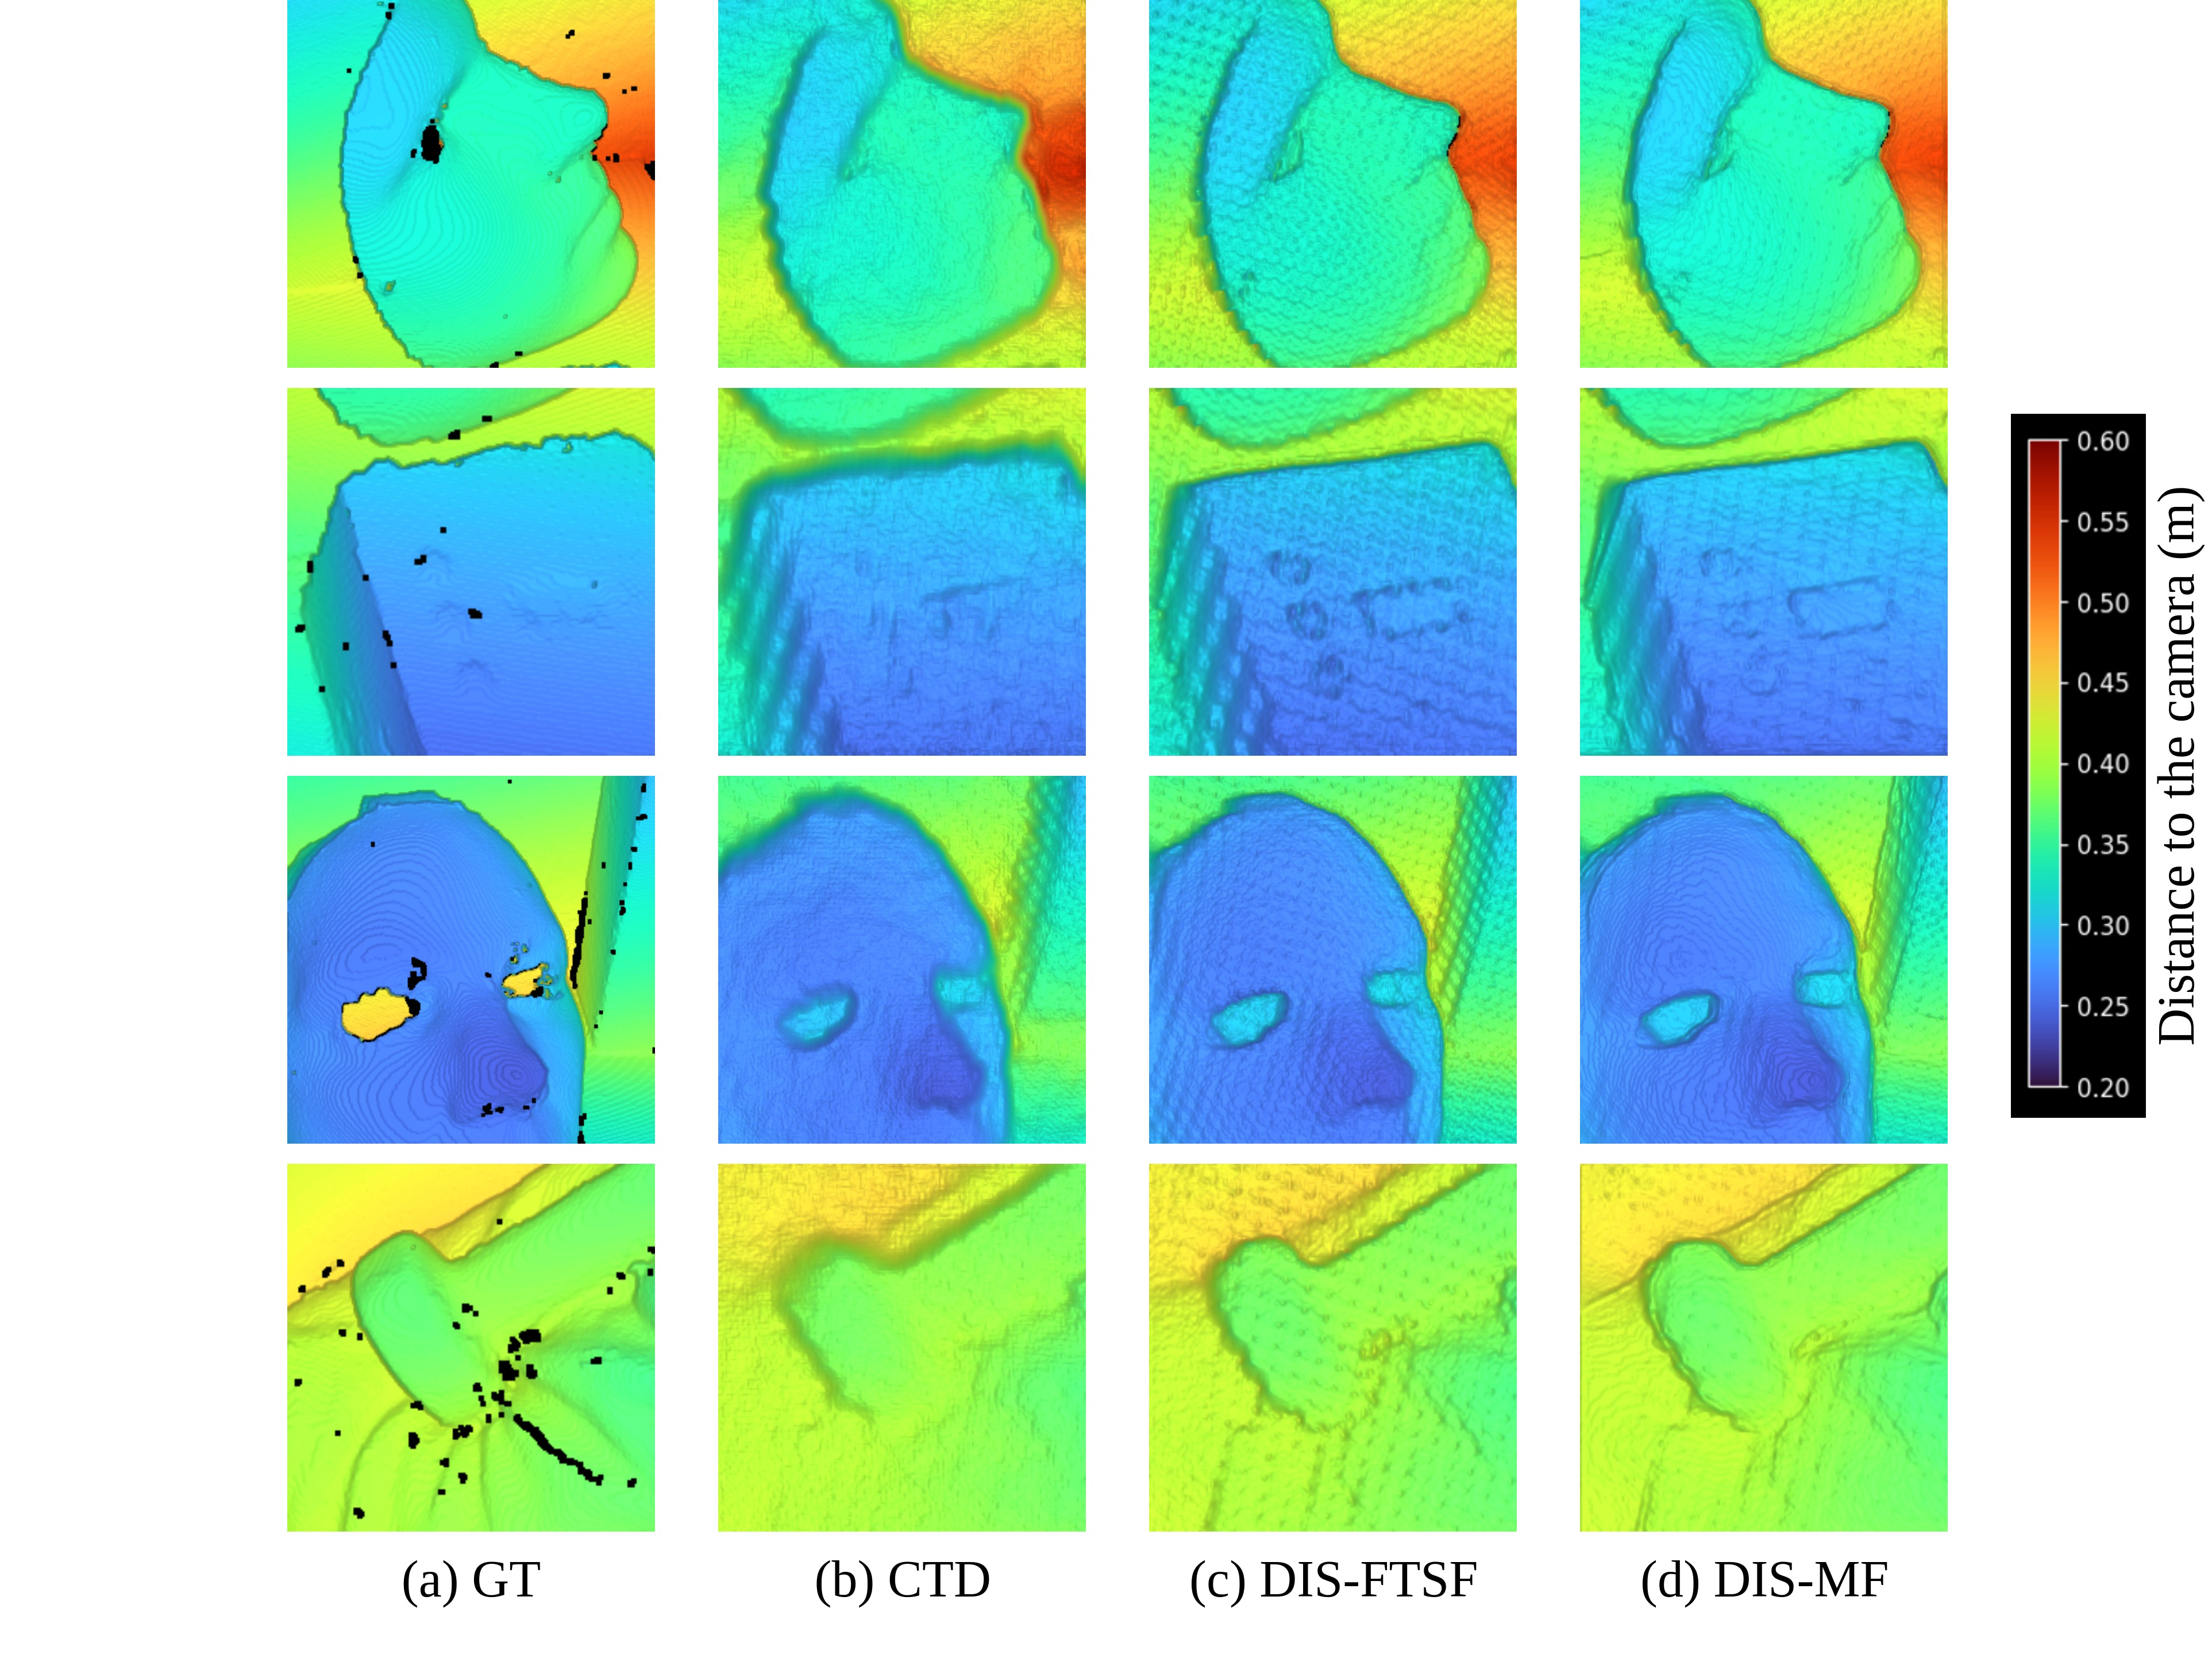
\includegraphics[width=1.0\linewidth]{images/chapter2/supp_figures/rendered_real.jpg}
    \end{center}
   \caption{Qualitative analysis of the depth maps rendered in OpenGL~\cite{shreiner2013opengl} and presented in the Turbo color map~\cite{mikhailov2019turbo}. Samples are taken from the real dataset. This analysis shows how our models outperform the state-of-the-art model, CTD~\cite{riegler2019connecting}, in preserving details of the 3D objects and producing sharp edges. It is noticeable that in some regions (\eg, the top edge of the box in the second row in column (a)), ground truth depths are noisy, and it is due to the limitations of the 3D scanner we used to capture ground truth depths. Since all evaluated methods are self-supervised, their performances are not affected by the ground truth noise. (a)~Ground truth depth map. (b)~CTD~\cite{riegler2019connecting}. (c)~Our DIS-FTSF model. (d)~Our DIS-MF model. For further information about 3D rendering of depth maps, refer to Section~\ref{sec:c2_additional_results}. The colorbar represents depth values in meters.}
    \label{fig:c2_rendered_real}
\end{figure}
